% Для подчеркивания важных моментов используйте, пожалуйста, команду \uline{} из пакета ulem

\documentclass[10pt, a4paper]{article}
\usepackage[T2A]{fontenc}
\usepackage[english, russian]{babel}

\usepackage{graphicx}
\graphicspath{{./figs/}}

\usepackage{titling}
\usepackage{wrapfig}
\usepackage{amsmath}
\usepackage{amssymb}
\usepackage{mathtools}
\usepackage{ulem}
\usepackage{physics}
\usepackage{upgreek}
\usepackage{sectsty}
\usepackage{color, soul}
\usepackage[dvipsnames]{xcolor}
\usepackage{indentfirst}
\usepackage[colorlinks=true,allcolors=blue]{hyperref}
\sectionfont{\centering}

\usepackage{chngcntr}
\counterwithin{figure}{section}
\numberwithin{equation}{section}

\usepackage{geometry}
 \geometry{
 a4paper,
 margin=25mm,
 }

\newcommand{\lambdabar}{{\mkern0.75mu\mathchar '26\mkern -9.75mu\lambda}}

\newcommand{\Tokman}{~[Токман, 2016]}
\newcommand{\Sidorov}{~[Сидоров, 2017]}

\title{Билеты к кандидатскому экзамену по физике плазмы: программа-минимум}
\date{}

\let\stdsection\section
\renewcommand\section{\newpage\stdsection}

\begin{document}

\maketitle

\section{Термодинамика плазмы}

\subsection{Понятие плазмы, квазинейтральность, микрополя, дебаевский радиус, идеальная и неидеальная плазма}

\uline{Плазма} -- квазинейтральная система, содержащая положительные и отрицательные свободные частицы \cite{frank}. Плазма -- одно из 4 агрегатных состояний вещества (кроме твёрдого тела, газа, жидкости есть ещё, например, всякие конденсаты (Бозе-Эйнштейна)). Плазма -- сильно ионизированный газ. Характерное свойство плазмы — существование коллективных
движений, связанных с дальнодействующим характером кулоновского взаимодействия \cite{kroll}. Плазма -- квазинейтральный газ заряженных частиц~\cite{kotelnikov}. Плазма -- ионизованный газ, свойства которого определяются этой ионизацией\Tokman. Бывает полностью или частично ионизованной; низкотемпературной ($T<10$ эВ) и высокотемпературной ($T\gg10$ эВ); слабо- или сильностолкновительной (сравнивается частота столкновений с плазменной частотой).

\begin{table}[h!]
	\caption{Характерные случаи плазмы и её характеристики~\cite{kotelnikov}. \linebreak Последние две строки -- по\Tokman. Имеет смысл сравнивать $n$ с $n_\text{воздуха} \sim 10^{19}$ см$^{-3}$.	Для справки: $1\ eV \approx 11.6\ K$, энергия покоя электрона $m_e c^2 = 511\ keV$.}
	\label{tabular:typical_plasma}
	\begin{center}
		\begin{tabular}{|c|c|c|}
			\hline
			Вид плазмы & $n,\,cm^{-3}$ & $T,\,eV$ \\ \hline
			Солнечное ядро & $10^{26}$ & $10^3$ \\
			Солнечная корона & $10^4-10^8$ & $10^2$ \\
			Солнечный ветер & $5$ & $10-50$ \\
			Ионосфера Земли & $10^2-10^6$ & $0.1$ \\
			Межзвёздный газ & $1$ & $1$ \\
			Газовый разряд & $10^{6}-10^{14}$ & $1$ \\
			УТС & $10^{12}-10^{14}$ & $10^4-5\cdot10^4$ \\
			Лазерный/импульсный УТС & $10^{22}-10^{24}$ & $10^4-5\cdot10^4$ \\
			\hline
		\end{tabular}
	\end{center}
\end{table}

\uline{Квазинейтральность} -- электрически нейтральная <<в среднем>>, <<в достаточно больших объёмах или за большие промежутки времени>> \cite{frank}. Оценивают по: пространственные/временные масштабы разделения зарядов.

\begin{itemize}
	\item \uline{Плазменная частота}. Можно показать, что в простейшем случае (плоский конденсатор) или в общем (через ур. Максвелла, через плотность объёмного заряда) пространственного разделения зарядов [поляризация плазмы] возникают колебания с плазменной частотой $\omega_{pe} = \sqrt{\frac{4\pi n e^2}{m}}$ [электростатические/ленгмюровские колебания]. Она -- показатель временного разделения заряда.
	
	Уравнение Максвелла без магнитного поля:
	
	\begin{equation}
		\label{eq:circuital_law}
		\dv{\vb{E}}{t} + 4\pi \vb{j} = 0
	\end{equation}

	Считаем ионы неподвижными. Тогда ток связан с движением электронов: $\vb{j}=-en\vb{v}$, где $n$ -- концентрация электронов. Продифференцировав уравнение~\eqref{eq:circuital_law} и учитывая уравнение Ньютона ($\dot{m\vb{v}}=-e\vb{E}$) имеем:
	
	\begin{equation*}
		\dv[2]{\vb{E}}{t}+4\pi\dv{\vb{j}}{t} = 0
	\end{equation*}
	\begin{equation}
		\dv[2]{\vb{E}}{t}+\frac{4\pi e^2 n}{m}\vb{E} = 0 
	\end{equation}

	Это уравнение \textbf{продольных} плазменных колебаний с частотой $\omega_{pe}^2=4\pi e^2 n/m$.
	
	Для $N\sim 10^{16}$ см$^{-3}$ $E_\text{разделения зарядов} \sim 10^9$ В/см -- огромная величина. На каких расстояниях может нарушаться квазинейтральность? Например, когда $E_\text{разделения зарядов} \sim 10^3$ В/см -- достижимая величина.
	
	\item \uline{Дебаевский радиус} -- характерная длина электрической экранировки заряда в плазме [за счёт её квазинейтральности]: $\lambda_D = \sqrt{\frac{T}{8\pi ne^2}}$. По сути, она же -- показатель пространственного разделения, который должен быть $\sim \langle v \rangle/\omega_{pe}$. Дебаевский радиус есть радиус корреляции электрического поля -- вне его частицы ведут себя независимо.
	
	Ещё один способ определения: характерное расстояние, на которое могут разделиться заряды при тепловом движении. В таком случае радиус Дебая находится из энергетического соотношения:
	
	\begin{equation*}
		NT \approx W_{EM}
	\end{equation*}

	где $W_{EM}=E^2/8\pi$ -- плотность энергии статического поля разделения зарядов. Само поле оценивается из модели конденсатора как $E=4\pi e N \delta x$, где $\delta x$ -- расстояние между обкладками, а в нашем случае -- сам радиус Дебая. В итоге:
	
	\begin{align*}
		NT = 2\pi e^2 N \lambda_D^2 \\
		\lambda_D = \sqrt{\frac{T}{2\pi e^2 N}}		
	\end{align*}

	Обратите внимание, что числовой коэффициент во всех этих случаях получается разный.
\end{itemize}

\uline{Микрополя}. Хрен знает, что имеется в виду, мб стоит сказать про \uline{функцию распределения}. Под действием столкновений плазма максвеллизируется~\cite{kroll} [здесь -- нормированная на концентрацию]:

\begin{equation}
	f(v) = \sqrt{\left( \frac{m}{2\pi T}\right)^3} e^{-\frac{mv^2}{2T}}
\end{equation}

или

\begin{equation}
	f(E) = \frac{2\pi}{\sqrt{\left(\pi T\right)^3}}\sqrt{E} e^{-\frac{E}{T}}
\end{equation}

\uline{Идеальная и неидеальная плазма}. Вводят либо число частиц в дебаевской сфере (сфера с радиусом $\lambda_D$) $N = \frac{4\pi}{3}n\lambda_D^3$, либо обратный ему параметр неидеальности $g = \frac{1}{n\lambda_D^3}$~\cite{kroll}. Случай $g \ll 1$: плазма идеальна, число частиц в деб. сфере большое, энергия взаимодействия много меньше кинетической энергии частиц плазмы (коллективные эффекты $\gg$ одночастичные; кулоновским взаимодействием часто можно пренебречь). В этом случае её свойства, как газа, схожи с идеальным газом -- никакие две частицы этого газа заряженных частиц не взаимодействуют (поэтому <<идеальная>>).

Важно: $g \sim \frac{n^{1/2}}{T^{3/2}}$, стремление к нулю соответствует <<разряженной>> плазме. Отсюда следует другой вид критерия идеальности: $T \gg e^2 n^{1/3}$~\cite{kotelnikov}.

Важно: в идеальном газе взаимодействует МАЛО частиц, в идеальной плазме взаимодействуют МНОГО частиц (но очень слабо).

Покажем, как энергия взаимодействия связана с числом частиц в дебаевской сфере. Рассмотрим точечный заряд $q$ в плазме. Его потенциал в плазме из-за экранировки равен $\varphi = q/r\exp{-r/\lambda_D}$, однако в вакууме он равен $\varphi_{vac}=q/r$. Это значит, что разницу между $\varphi$ и $\varphi_{vac}$ cоздали все частицы плазмы, окружающие этот точечный заряд.
Значит, что энергия взаимодействия (электростатическая) точечного заряда со всеми остальными частица плазмы равна $q (\varphi - \varphi_{vac})$, где потенциал плазмы надо рассчитывать в точке нахождения точечного заряда, т.е. в точке $r=0$. В итоге получаем энергию взаимодействия $-q^2/\lambda_D$.
Видно, что эта энергия в общем случае отличается от оценки кулоновского взаимодействия $q^2/\langle r\rangle$, где $\langle r \rangle = n_e^{-1/3}$~---~среднее расстояние между частицами.

В случае, когда плазма действительно ведёт себя как плазма, а не газ, и экранирует заряды, отношение потенциальной энергии к кинетической рассчитывается следующим образом:

\begin{equation}
	\frac{W}{T} \approx \frac{e^2}{\lambda_D T} = \frac{8\pi n e^2}{T}\frac{1}{8\pi n\lambda_D} = \frac{1}{8\pi n \lambda_D^3}
\end{equation}

Заметим, что это отношение с точностью до численного множителя равно обратному числу частиц в дебаевской сфере. Таким образом, если плазма идеальная и число частиц в дебаевской сфере большое, то кинетическая энергия частиц (тепловая) много больше их потенциального взаимодействия, как в идеальном газе. Однако в обычном газе потенциальную энергию надо учитывать без экранировки и критерий идеальности действительно получается другим, а именно:

\begin{equation}
	\frac{W}{T} \approx \frac{e^2}{\langle r \rangle T} = \frac{e^2 n^{1/3}}{T} \ll 1
\end{equation}

\subsection{Условие термодинамического равновесия, термическая ионизация,\linebreak формула Саха, корональное равновесие, снижение потенциала ионизации}

Следующий параграф посвящён рассмотрению процессов ионизации и рекомбинации в общем виде и поиску равновесия/математического описания подобных плазменных процессов.

\uline{Термическая ионизация} -- ионизация, при которой необходимую энергию для отрыва электрона от атома дают столкновения между атомами вследствие повышения температуры.

\uline{Условие термодинамического равновесия}. Плазма -- открытая система (т.к. излучает, вылетает, ...). Работает принцип детального равновесия: скорости прямого (ионизация) и обратного (рекомбинация) процессов должны в нём быть равны.

\begin{itemize}

\item Рассмотрим следующую пару процессов: ионизация электронным ударом $\leftrightarrow$ рекомбинация при тройных столкновениях~\cite{frank}.

Их скорости: $w_{ion} = k_{ion}n_an_e$ и $w_{rec} = k_{rec}n_in_e^2$ соответственно. $w_{ion}$ и $w_{rec}$ -- функции только температуры. Равновесие [закон действующих масс~\cite{frank}]:
 
\begin{equation} \label{eq:detailed_balance}
	K = \frac{k_{ion}}{k_{rec}} = \frac{n_in_e}{n_a},
\end{equation}

где $K$ -- константа равновесия. 

\item Рассмотрим следующую пару процессов: ионизация излучением $\leftrightarrow$ рекомбинация при двойных столкновениях с излучнием~\cite{frank}.

Их скорости: $w_{ion, rad} = k_{ion, rad}n_aI$ и $w_{rec, rad} = k_{rec, rad}n_in_e$ соответственно. $w_{ion}$ и $w_{rec}$ -- функции только температуры. Равновесие:

\begin{equation}
	\frac{k_{ion, rad}I}{k_{rec, rad}} = \frac{n_in_e}{n_a}.
\end{equation} 

\end{itemize}

Следовательно, общий вид условия термодинамического равновесия ионизации:

\begin{equation}
	K = \frac{k_{ion}}{k_{rec}} = \frac{k_{ion, rad}I}{k_{rec, rad}} = \frac{n_in_e}{n_a}
\end{equation}

Важно: если плазма всё-таки закрытая система, то условие выполняется автоматически. Если открытая, то может реализоваться ситуация, что ионизация и рекомбинация идут по разным путям (электронным ударом и с излучением соответственно). 

В таком случае балансное уравнение на концентрацию электронов имеет следующий простой вид:

\begin{equation}
	\frac{\partial n_e}{\partial t} = k_{\text{ион}}n_en_a-k_{\text{рек}}n_en_i,
\end{equation}

откуда следует, что равновесная [стационарная] концентрация электронов и ионов определяется формулой Эльверта:

\begin{equation}
	\alpha = n_i/n_a = k_{\text{ион}}/k_{\text{рек}}
\end{equation}

Это выражение называется также \uline{корональным равновесием}~\cite{kotelnikov}, т.к. реализуется в солнечной короне. 

Важно: степень ионизации не зависит от плотности плазмы.

Для равновесной ионизации [термодинамически равновесной плазмы], однако, существует фундаментальное \uline{уравнение Саха}, описывающее степень ионизации плазмы как функции температуры, давления и энергии ионизации атомов.

Условия применимости: ионизация и рекомбинация проходят по одному и тому же пути, плазма рассматривается как идеальный газ (при не слишком низких и не слишком высоких плотностях), кулоновская энергия мала по сравнению с тепловой [идеальная плазма]. 

Вывод~\cite{frank}:

Число электронов с импульсом от $\vec{p}$ до $\vec{p}+\vec{dp}$ в объёме $V$:

\begin{equation*}
	dN_e = d\Gamma(p)/V_{el} \cdot P(\varepsilon) = 4\pi p^2 Vdp\cdot \frac{1}{h^3} \cdot g_e e^{-\frac{\varepsilon}{T}},
\end{equation*}

где $d\Gamma(p)$ -- объём фазового пространства для частицы с импульсом от $\vec{p}$ до $\vec{p}+\vec{dp}$ ; $V_{el} = h^3$ -- элементарный объём фазового пространства; $P(\varepsilon)$ -- вероятность наличия частицы с заданной энергией. Здесь $g_e$ -- статистический вес, т. е. число состояний с одинаковой энергией, различающихся внутренними степенями свободы. $\varepsilon = I_p + \frac{p^2}{2m}$, где $I_p$ -- потенциал ионизации. Тогда число свободных электронов на один атом в определенном
квантовом состоянии:

\begin{equation*}
	N_e^{*} = \int_{0}^{\infty} dN_e = Vg_e\frac{(2\pi mT)^{3/2}}{h^3}e^{-\frac{I_p}{T}}
\end{equation*}

Полное число электронов получается умножением на число атомов в одном квантовом состоянии и заменой $V$ на объём, приходящийся на число ионов в определённом квантовом состоянии ($1/\frac{n_i}{g_i}$):

\begin{equation*}
	N_e = N_e^{*} \cdot N_a/g_a = \frac{g_i}{n_i} g_e\frac{(2\pi mT)^{3/2}}{h^3}e^{-\frac{I_p}{T}} \cdot \frac{N_a}{g_a}
\end{equation*}

Отсюда следует, что

\begin{equation} \label{eq:Saha}
	\frac{n_en_i}{n_a} = \frac{N_en_i}{N_a} = \frac{g_eg_i}{g_a} \frac{(2\pi mT)^{3/2}}{h^3}e^{-\frac{I_p}{T}}
\end{equation}

Классический вид уравнения Саха -- это как раз выражение~\ref{eq:Saha}. Часто, однако, оно записывается для случая многоступенчатой ионизации:

\begin{equation*}
	\frac{n_en_{i+1}}{n_i} = \frac{g_eg_{i+1}}{g_i} \frac{(2\pi mT)^{3/2}}{h^3}e^{-\frac{I_p^{(i)}}{T}}
\end{equation*}

Применимость: [астрофизика] Равновесная ионизация, описываемая уравнением Саха, объясняет эволюцию в ранней Вселенной. После Большого взрыва все атомы были ионизированы, оставив в основном протоны и электроны. Согласно подходу Саха, когда Вселенная расширилась и остыла так, что температура достигла примерно 3000 К, электроны рекомбинировали с протонами, образуя атомы водорода. В этот момент Вселенная стала прозрачной для большей части электромагнитного излучения. При исходной температуре $T = 3000 K$ с красным смещением примерно 1000 отсюда следует реликтовое излучение с $T = 3 K$, которое пронизывает всю Вселенную сегодня. 

Орбита сильно возбуждённого электрона далеко удалена от ядра, и на него влияют другие частицы. Электроны, окружающие атом, всё сильнее экранируют поле ядра, и когда радиус электронной орбиты превышает масштаб экранирования, сила притяжения атомного электрона к ядру начинает падать с расстоянием по экспоненциальному закону В таком при $r>\lambda_D$ связанные состояния не реализуются, и электрон становится свободным при энергии возбуждения, меньшей потенциала ионизации изолированного атома. Происходит как бы \uline{снижение потенциала ионизации}. Главное квантовое число $n$ последнего возбуждённого состояния можно оценить из условия $n^2a_0 \sim \lambda_D$ или $n \sim 10^4\sqrt{\lambda_D(\text{см})}$.

\subsection{Вырождение плазмы, статистика Больцмана и Ферми—Дирака, модель Томаса—Ферми}

\uline{Вырожденная [квантованная] плазма}: $T \leq \varepsilon_F$, где $\varepsilon_F$ -- энергия Ферми [максимально возможная энергия для фермиона при $T=0$]. Невырожденная плазма/описываемая классической физикой: $T \gg \varepsilon_F$. [Вырожденная = т.к. кв. состояния электронов вырождены по энергии, на каждом уровне их по два].

Новым эффектом в вырожденной плазме является обменное взаимодействие, не имеющее аналога в классической физике~\cite{kotelnikov}.

Важно: до экстремально низких температур ионы -- классические.

Слегка другой подход по\Tokman: плотность частиц в фазовом объёме в классическом случае: $\left( \frac{1}{\Delta p^3}\right)_{classic} = \frac{N}{p_T^3} = \frac{N}{m^3v_T^3}$; в квантовом: $\left(\frac{1}{\Delta p^3}\right)_{quantum} = \frac{V}{2 \pi \hbar^3}$ [следует из периодичности г.у. для рассматриваемого объёма]. Как правило, $\left( \frac{1}{\Delta p^3}\right)_{classic} \ll \left(\frac{1}{\Delta p^3}\right)_{quantum}$. Когда за счёт $N\uparrow$ достигает равенства, то надо учитывать квантовые эффекты и статистика Максвелла-Больцмана $\rightarrow$ статистика Ферми-Дирака. Условие классической статистики: $\frac{mv_T}{\hbar} = \lambda_D^{-1} \gg n^{1/3}$ ($\lambda_D$~---~длина волны де Бройля)

\uline{Распределение Больцмана} описывает распределение частиц в условиях термодинамического равновесия идеальной невырожденной плазмы:

\begin{equation}
	n = n_0e^{-\frac{\varepsilon}{T}}
\end{equation}

\uline{Распределение Ферми-Дирака} используется для описания вырожденной плазмы:

\begin{equation}
	f(\varepsilon) = \frac{1}{e^{\frac{\varepsilon-\varepsilon_F}{T}}+1}
\end{equation}

В пределе $T\rightarrow 0$ с вероятностью 1 заняты низшие состояния с энергией $\varepsilon \leq \varepsilon_F$; при $T \gg \varepsilon_F$ и $\varepsilon \gg \varepsilon_F$ распределение Ферми—Дирака переходит в распределение Больцмана.

Квантовые эффекты проявляются тогда, когда расстояние между частицами соразмерно с длиной волны де Бройля, то есть когда волновые функции частиц соприкасаются, но не перекрываются. [Вики]

Можно описывать плазму с помощью квантовомеханической \uline{модели Томаса-Ферми} в случаях, когда не работает модель Саха (вырожденная плазма; неидеальная плазма, большое число ионов)~\cite{kalitkin}. Можно даже сказать, что обобщенная модель Саха описывает газовую плазму, а модель Томаса-Ферми -- жидкую плазму. Переход между этими состояниями выше критической точки не является фазовым, а происходит плавно. 

\section{Элементарные процессы}

Часто для описания плазмы используют разбиение процессов на соударения и пролёт между соударениями. Такой подход, строго говоря, не применим для соударения заряженных частиц. При этом самыми вероятными (= важными) являются парные столкновения\Tokman. 

\subsection{Столкновения заряженных частиц, дальнодействие, частоты столкновений, столкновения электронов с атомами (упругие и неупругие), столкновения тяжёлых частиц. [Терминология]}

Соударения делятся на:
\begin{itemize}
	\item неупругие/неупругие первого рода -- возбуждение -- суммарная поступательная энергия частиц уменьшается;
	\item упругие [внутреннее состояние не меняется, обмен поступательной энергией] -- поступательная энергия частиц не меняется;
	\item сверхупругие/неупругие второго рода -- девозбуждение -- поступательная энергия частиц увеличивается~\cite{raizer}.
\end{itemize}

Как правило, упругие столкновения электрон испытывает намного чаще, чем неупругие. Поэтому для проводимости и поглощательной способности ионизированного газа, а также для диффузии электронов важнейшую роль играют именно упругие столкновения~\cite{raizer}.

Основные термины: длина свободного пробега [см], среднее время между соударениями [с], частота столкновений [Гц], эффективное сечение процессов [см$^2$]. 

Дифференциальные термины: дифференциальное сечение (рассеяния) [см$^2$].

Интегральные термины: транспортное сечение [см$^2$] и эффективная частота столкновений [Гц].

\subsubsection{Основные термины}

\uline{Эффективное сечение}. Согласно~\cite{raizer}: $\sigma(v) = \frac{\nu}{Nv}$, где $\nu$ -- число соударений в секунду [частота]; $N$ -- плотность налетающих частиц; $v$ -- скорость налетающих частиц. Для газокинетических столкновений его можно оценить как $\sigma \approx \pi(r_1+r_2)^2$, где $r_1$ и $r_2$ -- характерные радиусы частиц. Согласно~\cite{astap}: $\sigma=\int_{0}^{\infty} 2\pi \rho P(\rho) d\rho$, где $\rho$ -- прицельный параметр, $P(\rho)$ -- вероятность рассеяния (зависит от конкретных реагентов). 

\uline{Частота столкновений}: $\nu = N\left\langle v\sigma(v)\right\rangle $. В случае максвеллизации в газе из молекул одного сорта: $\nu = \sqrt{2}N\overline{v}\pi d^2$. 
Если рассматривается сразу несколько процессов, например, разные сорта газа или возбуждение нескольких уровней, то

\begin{equation*}
	\nu = \sum_{i}N_i\overline{v}\sigma_i
\end{equation*}

\uline{Среднее время между соударениями}: $\tau = 1/\nu$.

\uline{Длина свободного пробега}: $l = 1/(N\sigma)$.
Для разных сортов газа или рассмотрения нескольких процессов:

\begin{equation*}
	\frac{1}{l} = \sum_{i}\frac{1}{l_i}\approx\sum_{i}N_i\sigma_i
\end{equation*}

\subsubsection{Дифференциальные и интегральные термины}

Для ввода остальных терминов надо более подробно рассмотреть случай парного столкновения.	

\begin{quotation}
	Важно: Совершенно необязательно рассматривать в классической плазме взаимодействие в классическом виде. Та же ионизация -- квантовый процесс (хоть может быть описана и в классическом виде тоже)\Tokman.
\end{quotation}

{\bfseries \large I. Частоты столкновений.} Рассмотрим два сорта частиц $\alpha$ и $\beta$ ($e, i, n$) и перейдём в систему центра масс:

\begin{figure}[h!]
	\begin{center}
		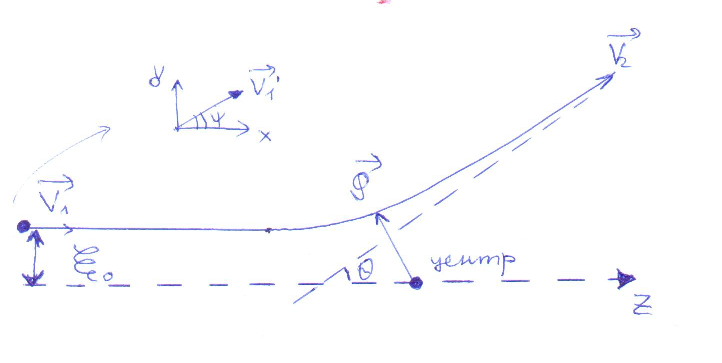
\includegraphics[width=0.6\linewidth]{scattering_simple.pdf}
	\end{center}
	\caption{Рисунок из лекций}
	\label{fig:scattering}
\end{figure}

\begin{equation} \label{eq:center_mass}
	\vec{R} = \frac{m_\alpha\vec{r_\alpha}+m_\beta\vec{r_\beta}}{m_\alpha+m_\beta}
\end{equation}

\begin{equation*}
	\vec{\rho} = \vec{r_\alpha}-\vec{r_\beta};\,
	\vec{V} = \dot{\vec{R}};\,
	\vec{v} = \dot{\vec{\rho}}
\end{equation*}

Можно показать, что кинетическая энергия равна

\begin{equation*}
	K = m_\Sigma\frac{V^2}{2}+\mu_{\alpha\beta}\frac{v^2}{2},
\end{equation*}

где $\mu_{\alpha\beta}$ -- приведённая масса. 

Гамильтониан:

\begin{equation*}
	H = \frac{p^2}{2\mu_{\alpha\beta}}+U(\abs{\vec{\rho}});\,
	\vec{p} = \mu_{\alpha\beta}\vec{v}
\end{equation*}

Также надо учесть законы сохранения: 1. Поскольку рассматривается упругое рассеяние: $U(\pm \infty) = 0, v_1 = v_2 = 0$ 2. Сохранение момента импульса (система замкнута): $\vec{L} = \vec{\rho} \times \vec{p} = \vec{\rho} \mu_{\alpha\beta} \vec{v} = const$.

Более-менее строгий вывод:

\begin{equation*}
	\Delta p_\alpha = \mu_{\alpha\beta} \Delta v_\alpha
\end{equation*}

\begin{equation*}
	\Delta v_\alpha = \Delta v_{\alpha_{z}} = -(1-cos\theta)v
\end{equation*}

Тогда

\begin{equation}
	\label{eq.2.kinetic_energy}
	\Delta K_\alpha = \mu_{\alpha\beta}\vec{V}\Delta\overrightarrow{ p_\alpha} 
\end{equation}

В силу симметрии можно записать:

\begin{equation*}
	\theta = \pi - 2 \int_{\rho_{min}}^{\infty}\frac{\xi_0 dr}{\rho\sqrt{1-\frac{\xi_0^2}{\rho^2}-\frac{U(\rho)}{K_0}}}
\end{equation*}

Таким образом, результат [если не требуется точная зависимость]: $\theta = \theta(v, \xi_0)$.

{\bfseries \large II. Столкновения электронов с атомами [упругие].} Перейдём от парного столкновения к рассмотрению рассеивающего поток частиц центра. Цель: определить среднее число частиц $dN'$, улетающих в единицу времени в элемент телесного угла при заданных $\theta$ и $\psi$.

Очевидно, что $\frac{dN'}{dt} \sim nv;\, \frac{dN'}{dt} \sim d\Omega$. Введём коэффициент пропорциональности, имеющий размерность площади:

\begin{equation*}
	\frac{dN'}{dt} = d\Omega\cdot nv \cdot \sigma_{\alpha\beta}(\theta, v)
\end{equation*}

Так как в процессе столкновения число частиц не изменяется, то число частиц, которое после рассеяния попадает в элемент телесного угла $d\Omega$, равно числу частиц, которые налетают на рассеивающий центр с прицельным параметром $\xi_0$, т.е.:

\begin{equation*}
	\frac{dN'}{dt} = dS \cdot nv = \xi_0 d\xi_0 d\psi   \cdot nv
\end{equation*}

Приравнивая, получаем:

\begin{equation*}
	\sigma_{\alpha\beta} d\Omega = \sigma_{\alpha\beta} sin\theta \cdot d\theta \cdot d\psi = d \psi \cdot \xi_0 \cdot d\xi_0
\end{equation*}

Тогда (добавляем модуль из соображений того, что ранее писали без учёта знаков):

\begin{equation} \label{eq:transport_cs}
	\sigma_{\alpha\beta} = \frac{\xi_0}{sin\theta}\abs{\frac{d\xi_0}{d\theta}}
\end{equation}
где $d\xi_0/d\theta$ надо понимать в смысле $(d\theta/d\xi_0)^{-1}$, т.к. при решении задачи мы обычно ищем зависимость угла рассеяния от прицельного параметра, а не наоборот.

$\sigma_{\alpha\beta}$ называется \uline{диффференциальным сечением рассеяния} и имеет смысл той площади, с которой частицы летят в определённый угол.

Дифференциальное сечение важно, поскольку в эксперименте положение детектора соответствует какому-то телесному углу и нужен пересчёт измеренных данных в физические характеристики процесса.

Полное сечение рассеяние определяется как интеграл от дифференциального сечения по всем телесным углам:

\begin{equation} \label{eq:total_cs}
	S_{\alpha\beta} = \int \sigma_{\alpha\beta} d\Omega = 2 \pi \int_{0}^{\pi} \sigma_{\alpha\beta} sin\theta \cdot d\theta
\end{equation}

Полное число частиц сорта $\alpha$, сталкивающихся в единицу времени в единице объёма с частицами сорта $\beta$, равно

\begin{equation*}
	\frac{dn_\alpha}{dt} = n_\alpha n_\beta S_{\alpha\beta} v = n_\alpha\nu_{\alpha\beta},
\end{equation*}

где $\nu_{\alpha\beta}$ -- частота столкновений = полное число столкновений частицЫ сорта $\alpha$ с частицами сорта $\beta$ в единицу времени.

Изменение импульса в единицу времени в единице объёма:

\begin{equation*}
	\left\langle \Delta \vec{p_\alpha}\right\rangle = \left\langle -\mu_{\alpha\beta}(1-cos\theta)v \right\rangle = -\mu_{\alpha\beta}n_\alpha n_\beta \int d^3v v \vec{v} S_{\alpha\beta}^t(v) = -\mu_{\alpha\beta}n_\alpha\int d^3v \vec{v}\nu_{\alpha\beta}^t,
\end{equation*}

где $S_{\alpha\beta}^t(v)$ -- тот же интеграл $S_{\alpha\beta}$ из (\ref{eq:total_cs}), но с весом $1-cos\theta$ (аналогично с $\nu_{\alpha\beta}^t$). Эти величины называются \uline{транспортными}\Tokman.

\begin{quotation}

Другой подход\cite{raizer}: \uline{Транспортным сечением} реакции называется выражение $\sigma_{tr} = \sigma_c(1-\langle {cos\theta}\rangle$, где $\sigma_c$ -- полное сечение рассеяния, а $\theta$ -- угол между конечной и начальной скоростью рассеянной частицы. Выражение $\nu_m = Nv\sigma_{tr}$ носит название \uline{эффективной частоты столкновений}. Ей соответствует длина пробега $l_m = 1/(N\sigma_{tr})$. При изотропном рассеянии эти величины совпадают с полными сечением, частотой и длиной пробега. При ситуации, когда в основном рассеяние происходит ``вперёд'' (т.е. скорость налетающей частицы после взаимодействия направлена практически в ту же сторону), транспортное сечение и эффективная частота столкновений меньше истинных. Если рассеяние происходит ``назад'', то -- больше. Таким образом, данные величины введены для индикации отличия рассеяния от изотропного.

Считая тяжёлые частицы (атомы, молекулы, ионы) неподвижными, можно показать~\cite{raizer}, что потери энергии $\delta_\varepsilon = \frac{2m}{M}(1-\langle cos\theta\rangle)$, что при переходе к ``эффективным'' соударениям даёт долю потерянной энергии в одном эффективном взаимодействии в $\frac{2m}{M}$. 

Важно: это очень малая величина, поэтому температура электронов (которые, \uline{как правило}, греются) и ионов сильно отличаются/долго выравниваются.

\end{quotation}

Изменение энергии в единицу времени в единице объёма:

\begin{equation*}
	\left \langle \Delta K_\alpha \right \rangle = - \varkappa_{\alpha\beta} (1-cos\theta) (K_\alpha-K_\beta),
\end{equation*}

где $\varkappa_{\alpha\beta} = \frac{2m_\alpha m_\beta}{(m_\alpha+m_\beta)^2}$.

Если мы хотим использовать величины, иллюстрирующие множество процессов, то в выражениях, например, для транспортного сечения надо добавить $\sum$ и перейти к $\Delta E_j$. 

Важно: Рассеяние на атоме можно считать классической задачей, если: $\lambda_\text{де Бройля} = \frac{\hbar}{m_\alpha v_T} \ll r_{min} \sim a_{Bohr} = \frac{\hbar^2}{m_e e^2}$, что соответствует $K_e \gg I$ [потенциала ионизации] -- тогда задача классическая. В случае ионизации работает классика, если передаётся энергии более чем $I$ [отсюда тоже можно взять оценку\Tokman].

Важно: у некоторых атомов и молекул наблюдаются глубокие минимумы сечений в области энергий $\varepsilon \sim 0.1-1$ эВ --- \uline{эффект Рамзауэра} \cite{raizer} (принципиально квантовый), аналогичный эффекту пятна Пуассона в оптике. Роль ``экрана'' для электрона играет атом. Если длина волны де Бройля электрона сравнима с размером атома, то в результате дифракции электрона за атомом возникает максимум электронной волны — электрон ``огибает'' атом без рассеяния на нём.

\begin{quotation}
	
	Точное решение квантово-механической задачи рассеяния электрона на атоме дает следующее выражение для транспортного сечения упругого рассеяния:
	
	\begin{equation*}
		\sigma_{tr}^{quantum} = 4\pi \left(L^{2}+\frac{4}{5}\frac{\pi \alpha L}{a_{Bohr}}\frac{m_ev}{\hbar}+\frac{\pi^{2}}{6}\frac{\alpha^{2}}{a_{Bohr}^{2}}\left( \frac{m_ev}{\hbar}\right) ^{2} \right), 
	\end{equation*}
	
	где $L$ -- т.н. ``длина рассеяния''; $\alpha$ -- поляризуемость атома [входит в потенциал взаимодействия].
	
	Слагаемые соответствуют: короткодействующему взаимодействию (1), дальнодействующему потенциалу (3) и интерференции двух этих эффектов [проявляются волновые свойства электрона; может быть отрицательным].
	
	\begin{itemize}
		\item[$\oplus$] И. Мак-Даниэль ``Процессы столкновений в ионизированных газах'', гл. 3, \S 15.
	\end{itemize}
	
\end{quotation}

{\bfseries \large III. Столкновения заряженных частиц. Дальнодействие.} Рассмотрим парные кулоновские столкновения.

Берём из термеха \uline{формулу Резерфорда}:

\begin{equation} \label{eq:Rutherford}
	\xi_0 = r_s ctg\frac{\theta}{2},
\end{equation}

где $r_s = \frac{e^2}{\mu_{\alpha\beta}v_\infty^2}$ -- называется кулоновским радиусом (при нём потенциальная энергия взаимодействия сравнима с кинетической энергией относительного движения, а лёгкая частица отклоняется в результате взаимодействия на угол $\theta=\frac{\pi}{2}$\cite{raizer}). Тогда из (\ref{eq:transport_cs}):

\begin{equation*}
	\sigma_{\alpha\beta} = \frac{\xi_0}{\sin\theta}\abs{\frac{d\xi_0}{d\theta}} = r_s^2\frac{\cos\frac{\theta}{2}}{2\sin^2\frac{\theta}{2}\cos\frac{\theta}{2}}\frac{1}{2\sin^2\frac{\theta}{2}} = \frac{r_s^2}{4\sin^4\frac{\theta}{2}}
\end{equation*}

В таком случае (\ref{eq:total_cs}):

\begin{equation*}
	S_{\alpha\beta}^t = 2\pi\int_{\theta_{min}}^{\pi}\frac{r_s^2}{4\sin^4\frac{\theta}{2}}\sin\theta(1-\cos\theta)d\theta = 2\pi r_s^2\int_{\theta_{min}}^{\pi} \frac{\cos\frac{\theta}{2}}{\sin\frac{\theta}{2}}d\theta = -4\pi r_s^2 \cdot \ln\left( \sin\frac{\theta_{min}}{2}\right) 
\end{equation*}

Проблема: бесконечно сильное столкновение (само по себе нефизично) + потенциально отсутствие распространения волн в плазме (опровергается экспериментом).

Расходится в области малых углов $\theta_{min}\sim\xi_{max}$, где $K\gg U$. Проведём аппроксимацию:

\begin{equation*}
	\sin\frac{\theta_{min}}{2}\approx \frac{\theta_{min}}{2} = \frac{1}{\left[ 1+\left( \frac{\xi_0^{max}}{r_s}\right)^2 \right]^{1/2}} \approx \frac{r_s}{\xi_0^{max}} \approx \frac{r_s}{\lambda_D}
\end{equation*}

Итак, 

\begin{equation*}
	S_{\alpha\beta}^t = 4\pi r_s^2 \cdot \ln\frac{\lambda_D}{r_s} = 4\pi r_s^2 L,
\end{equation*}

где $L$ -- \uline{кулоновский логарифм} (порядок величины: 15-17 в токамаке, обычно берут равным 10). Основной вклад в сечение дают рассеяния на малые углы. В этом и проявляется \uline{дальнодействие}: малые углы $\sim$ большие прицельные параметры. Важно: здесь не была учтена разница между средними скоростями электронов и ионов.

Кулоновский логарифм:

\begin{equation*}
	L = \ln\frac{\lambda_D}{r_s} \sim \ln\frac{(T/(ne^2))^{1/2}}{e^2/T} = \ln\frac{T^{3/2}}{n^{1/2}e^3}
\end{equation*}

\begin{equation} \label{eq:Coulomb_log}
	L_e = 23+\frac{3}{2}\ln(T_e)-\frac{1}{2}\ln(n); L_i = 23+
	\frac{3}{2}\ln(T_{i,e})-\frac{1}{2}\ln(n)
\end{equation}

$T_{i,e} = min(T_e, T_i)$, [$T$] = эВ, [$n$] = см$^{-3}$.

Частоты столкновений:

\begin{equation} \label{eq:freq_ee}
	\nu_{ee}^t = \frac{16\pi e^4 n}{m_e^2v_e^3}L_{ee},
\end{equation}

$v_e\sim v_T$ -- тепловая.

\begin{equation} \label{eq:freq_ei}
	\nu_{ei}^t = \frac{\nu_{ee}}{4},
\end{equation}

т.к. приведённая масса в два раза больше.

\begin{equation} \label{eq:freq_ii}
	\nu_{ii}^t = \frac{16\pi e^4 n}{m_i^2v_i^3}L_{ii}
\end{equation}

\begin{equation*}
	\nu_{ei} = \frac{4\pi e^4 n}{m^2v^3}L_{ee} \approx \frac{\omega_{pe}^4}{nv_{Te}^3}L_{ee} = \frac{\omega_{pe}}{n\lambda_D^3}L_{ee}
\end{equation*}

Условие идеальной плазмы: $n\lambda_D^3 \gg 1$, то $\nu_{ei} \ll \omega_{pe}$. $\nu_{ei}$ определяет коэффициент затухания плазменных колебаний.

Дополнение: В квантовой механике нет предельного параметра -- кажется, что нет и дифференциального сечения рассеяния. Однако в ней возможен такой же подход с разделением/заменой переменных, но уже в уравнении Шрёдингера (на движение ц. масс и относительно него). 

Знание сечений элементарных процессов (в т.ч. -- из квантовой механики) позволяет полностью описать систему в рамках данного подхода.

\subsection{Неупругие столкновения электронов с атомами. Ионизация, рекомбинация, перезарядка и прилипание. Возбуждение и диссоциация молекул электронным ударом}

\subsubsection{Ионизация}

\begin{equation}
	A + e \rightarrow A^{+} + 2e
\end{equation}

\uline{Потенциал ионизации} $I$ -- энергия связи электрона в атоме (ионе), которую необходимо затратить, чтобы эту связь разорвать. Соответственно, процесс ионизации носит пороговый характер. Вблизи $\varepsilon \approx I$ сечение ионизации можно аппроксимировать как: $\sigma = C(\varepsilon-I)$. Характерное сечение
ионизации $[С\times1 \text{эВ}]$ см$^2$, соответствующее $\varepsilon = I + 1\text{эВ}$, на два порядка
меньше сечений упругих соударений электронов. В максимуме сечение ионизации обычно в два или несколько раз меньше упругого при той же энергии~\cite{raizer}.

Для ионизации существует формула Томсона, которая выводится из классических соображений (разумеется, является достаточно грубым приближением). Рассматривается упругое соударение двух электронов: налетающего и ``связанного'' с атомом. Налетающий передаёт второму электрону энергию $\Delta\varepsilon$ (ионизация в данном случае определяется как случай $\Delta\varepsilon > I$). Тогда из (\ref{eq.2.kinetic_energy}):

\begin{equation*}
	\Delta \varepsilon = \mu \vec{V}\vec{v} (1-\cos\theta) = \frac{m_e}{2} \frac{v_1^2+v_2^2}{2} (1-\cos\theta) = \frac{\varepsilon}{2} (1-\cos\theta)
\end{equation*}

и из (\ref{eq:total_cs}) и (\ref{eq:Rutherford}):

\begin{equation*}
	\sigma_{ion}^{Th} = 2\pi\int\frac{r_s^2}{4\sin^4\frac{\theta}{2}}\sin\theta d\theta = \frac{\pi r_s^2}{2} \int\frac{4}{(1-\cos\theta)^2}d(\cos\theta) = 2\pi r_s^2\int_{I}^{\varepsilon}\frac{\varepsilon^2}{4\Delta\varepsilon^2}\frac{-2\Delta\varepsilon}{\varepsilon} = \frac{\pi e^4}{4\varepsilon^2}\frac{\varepsilon-I}{I}
\end{equation*}

[как-то возникла лишняя четвёрка -- не думаю, что это критично для экзамена, но в книгах в знаменателе её нет]

\textcolor{red}{Не очень понял вывод. Предлагаю другой вариант:}
Очевидно, что $\sin\theta = p_\perp/p$, где $p_\perp$~---~поперечный импульс, приобретённый частицей из-за рассеяния, а $p$~---~её полный импульс после рассеяния. Но так как рассеяние упругое, то $p$ равно начальному импульсу, т.е. $p=\sqrt{2m\varepsilon}$. Последнее верно из-за того, что на самом деле электрон рассеивается на связанном электроне в атоме, поэтому эффективная масса последнего равна массе атома и можно считать, что в лабораторной системе отсчёта атом неподвижен. Очевидно, что рассеивающий центр (связанный электрон в данном случае) приобретает такой же импульс по 3-му закону Ньютона, тогда $\varepsilon_b=p_\perp^2/2m$, где $\varepsilon_b$~---~энергия изначально связанного электрона после рассеяния. Дифференциальное сечение рассеяния $\dd\sigma$ равно $2\pi\xi_0\dd \xi_0$. Найдём прицельный параметр $\xi_0$ в приближении малых углов рассеяния:
\begin{align*}
	\sin\theta = \frac{p_\perp}{p} = \sqrt{\frac{\varepsilon_b}{\varepsilon}} ,\\
	\frac{e^2}{\varepsilon\xi_0} = \sqrt{\frac{\varepsilon_b}{\varepsilon}} ,\\
	\xi_0^2 = \frac{e^4}{\varepsilon \varepsilon_b}.
\end{align*}
В итоге имеем:
\begin{equation*}
	\dd\sigma = 2\pi\xi_0\dd\xi_0 = \pi\dd\xi_0^2 = \frac{\pi e^2}{\varepsilon\varepsilon_b^2}\dd\varepsilon_b
\end{equation*}
Полное сечение получаем интегрируя по $\varepsilon_b$ от энергии ионизации $I$ до энергии свободного электрона $\varepsilon$:
\begin{equation}
	\sigma = \frac{\pi e^2}{\varepsilon}\int_I^\varepsilon\frac{\dd \varepsilon_b}{\varepsilon_b^2} = \frac{\pi e^2}{\varepsilon}\left( \frac{1}{I} - \frac{1}{\varepsilon} \right) = \frac{\pi e^2}{\varepsilon^2}\frac{\varepsilon - I}{I}
\end{equation}

Для большей точности формулу представляют часто в виде~\cite{astap}:

\begin{equation*}
	\sigma_{ion}^{Th} = \pi a_I^2 f^{Th}(\varepsilon/I),
\end{equation*}

где $a_I = \frac{e^2}{I}$ -- радиус ионизации = расстояние, на котором энергия кулоновского взаимодействия равна потенциалу ионизации; $f^{Th}(x) = \frac{x-1}{x^2}$ -- безразмерная функция Томсона. Грубая оценка: $\sigma_{ion} = \pi a_I^2$. Т.к. энергия входит в виде $\varepsilon/I$, используются методы подобия, когда в каждом отдельном случае определяется вид функции $f^{Th}(x)$. 

Важно: для расчёта ионизации многоэлектронных атомов электронным ударом будет сумма таких выражений с весом в виде функции Хэвисайда (пороговость процесса).

Процесс ионизации в плазме осуществляется в основном электронами с энергией, заметно превосходящей температуру плазмы [т.н. ``хвост'' максвелловского распределения]~\cite{astap}. Поэтому ионизация становится заметной уже при температурах, достаточно малых по сравнению с потенциалами ионизации атомом (например, при $T=1$ эВ в водородной плазме с $I_p=13.6$ эВ).

Кроме того, может происходить \uline{многоступенчатая ионизация} -- т.е. ионизация через возбуждённые уровни, в несколько этапов. Такой процесс возможен для электронов с энергией меньше, чем потенциал ионизации. Сечение ионизации возбуждённого атома существенно выше, чем невозбуждённого. 

Можно рассматривать и ионизацию ионов. Очевидно, что для неё сечение процесса меньше, чем для атома (влияние положительного атомного остатка)~\cite{raizer}.

\subsubsection{Рекомбинация} \label{subsubsec:recombination}

\begin{equation}
	A^{+Z} + e + C \rightarrow A^{+(Z-1)} + C',
\end{equation}

где через $C$ и $C'$ обозначено состояние третьего тела (наличие которого необходимо для выполнения ЗСЭ) до и после реакции. Важно, что в качестве $C$ может выступать даже электронный остов рекомбинирующего иона~\cite{astap}. Может в результате излучать фотон -- фото-/радиационная рекомбинация.

Плотная холодная плазма (большой радиус кулоновского взаимодействия): доминирует трёхчастичная рекомбинация, разреженная горячая плазма: фоторекомбинация.

В результате баланса между ионизацией и рекомбинацией в плазме устанавливается ионизационное равновесие, характеризуемое определенным соотношением между концентрацией нейтральных и заряженных частиц, а также между концентрацией
ионов с различными зарядами. 

\uline{Трехчастичная рекомбинация} является процессом, детально обратным процессу ионизации:

\begin{equation*}
	A^{+Z} + 2e \rightarrow A^{+(Z-1)} + e 
\end{equation*}

Для вывода скорости рекомбинации через детальный баланс (ур.~\ref{eq:detailed_balance} и см., например, ~\cite{astap}), нужно использовать формулу Саха (ур.~\ref{eq:Saha}) и знать вид выражения для константы скорости соответствующей ионизации.

Используя их, можно показать, что скорости прямой и ступенчатой ионизации соотносятся как

\begin{equation}
	\frac{k_{\text{прям}}}{k_{\text{ступ}}} \approx \left(\frac{T}{I}\right)^{\frac{7}{2}}
\end{equation}

\uline{Диэлектронная рекомбинация} является наряду с трехчастичной и радиационной одним из основных процессов образования ионов меньшей кратности в плазме с достаточно низкой плотностью, где преобладают процессы парных соударений. Для реализации этого вида рекомбинации необходимо наличие у рекомбинирующего иона некоторого числа остаточных электронов, т.е. электронного остова, который берёт на себя избыток энергии рекомбинирующего электрона~\cite{astap, raizer}.

\begin{equation*}
	A^{+Z} + e \leftrightarrow A^{**}
\end{equation*}

Диэлектронная рекомбинация преобладает над трехчастичной рекомбинацией в достаточно разреженной плазме (малые $n_e$) и при достаточно высокой температуре плазмы.

\uline{Диссоциативная рекомбинация} состоит из двух этапов. Первый: объединение молекулярного иона $АВ^{+}$ и электрона в квазимолекулу, которая находится в сверхвозбужденном автоионизационном состоянии. Второй: переход в молекулу $AB$ (может и не существовать: инертные газы) или в два атома $A$ и $B$; один из них может быть и возбужденным. Это возможно, если потенциальная кривая какого-либо из состояний системы атомов $А^{*}+В$ пересекает потенциальную кривую иона $AB^{+}$.

\begin{equation*}
	AB^{+} + e \leftrightarrow A^{*}+B \rightarrow AB | A+B
\end{equation*}

Системы $AB^{+}+e$ и $A^{*}+B$ при междуядерном расстоянии около $r_m$ имеют одинаковые энергии (см. рис. \ref{fig:diss_recomb}). Поэтому возможен самопроизвольный переход из первой конфигурации во вторую. 

\begin{figure}[h!]
	\begin{center}
		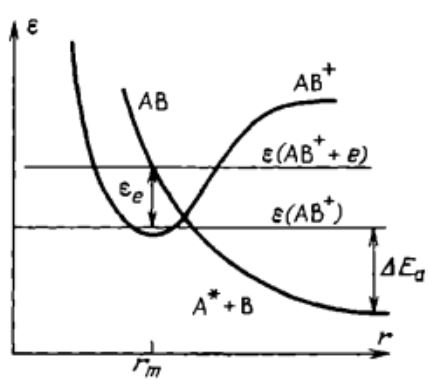
\includegraphics[width=0.3\linewidth]{diss_recomb.jpg}
	\end{center}
	\caption{Схема потенциальных кривых для случая диссоциативной рекомбинации}
	\label{fig:diss_recomb}
\end{figure}

Коэффициент диссоциативной рекомбинации равен:

\begin{equation}
	\beta_{\text{дисс\textunderscore рекомб}} = k_{\text{захв}}\frac{\omega_{\text{стаб}}}{\omega_{\text{стаб}}+\omega_{\text{авто}}} = \frac{k_{\text{захв}}}{\omega_{\text{авто}}}\frac{\omega_{\text{стаб}}\omega_{\text{\text{авто}}}}{\omega_{\text{стаб}}+\omega_{\text{авто}}},
\end{equation}

где $\omega_{\text{стаб}}$ -- вероятность стабилизации [c$^{-1}$] (обратное время жизни состояния); $\omega_{\text{авто}}$ -- вероятность автоионизации; $k_{\text{захв}}$ -- константа скорости захватов.

$\omega_{\text{стаб}} \sim v_a/a$ -- отношение скорости разлёта атомов квазимолекулы к их характерному размеру. $\omega_{\text{стаб}} \sim 10^{14}$ c$^{-1}$ -- очень быстрый процесс (для сравнения скорость высвечивания кванта $v_{q} \sim 10^{8}$ c$^{-1}$).

\subsubsection{Перезарядка}

Столкновения заряженных тяжелых частиц с атомами и молекулами зависит от состояний сталкивающихся частиц. Столкновения ионов с атомами в низкотемпературной плазме относятся к типу медленных столкновений, которые характеризуются особенностями квазимолекулы, образованной сталкивающимися ионом и атомом~\cite{astap}.

Важным условием для взаимодействия тяжёлых частиц [но не только их] является условие быстроты воздействия~\cite{astap}. Грубо говоря, при медленном столкновении атома с частицей плазмы электронные оболочки атома успевают за время столкновения подстроиться под движение налетающей частицы и затем вернуться в исходное положение после окончания столкновения. Говорят, что частицы движутся по адиабатическим молекулярным термам, не переходя в другие атомные состояния. Таким образом, условием служит малость отношения частоты к частоте пролета возмущающей частицы: 

\begin{equation} \label{eq:Messi}
	M = \frac{\rho \omega}{v} \ll 1,
\end{equation}

$\rho$ -- прицельный параметр, $v$ -- относительная скорость, $\omega$ -- частота перехода.

Обратное условие, отвечающее малости вероятности перехода при медленном столкновении, называется адиабатическим критерием Месси, а сам параметр $M$, входящий в условие (\ref{eq:Messi}) -- \uline{параметром Месси}.

Можно рассмотреть простейший случай -- двухуровневую квазимолекулу (см. рис. \ref{fig:terms_quasimol}). Общее решение, однако, при произвольных скоростях изменения потенциалов
взаимодействия невозможно получить в аналитическом виде. Приближённое решение можно получить с использованием борновского приближения. Борновское приближение расходится при малых прицельных параметрах пролета. В результате получается
функция, описывающая плавный переход от борновского предела
к экспоненциальному спаду, содержащему в экспоненте параметр Месси (характерные изменения в виде переходов в зависимости от скорости процесса -- см. рис. \ref{fig:transitions_2levels}).

\begin{figure}[h]
	\begin{center}
		\begin{minipage}[h]{0.49\linewidth}
			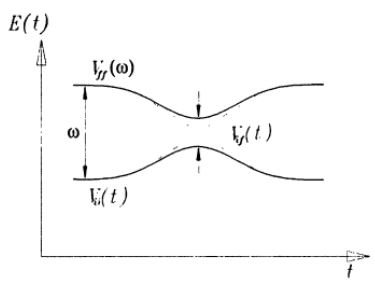
\includegraphics[width=1\linewidth]{heavy_particle.jpg}
			\caption{Эволюция во времени термов квазимолекулы, образованной
сталкивающимися тяжёлыми частица} 
			\label{fig:terms_quasimol}
		\end{minipage}
		\hfill
		\begin{minipage}[h]{0.49\linewidth}
			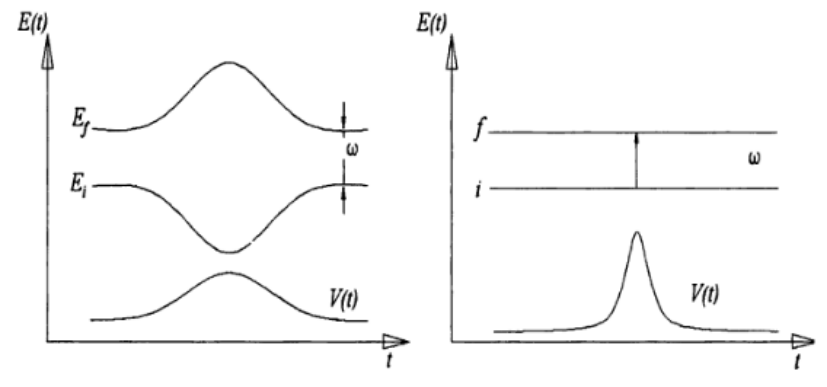
\includegraphics[width=1\linewidth]{2levels_transition.png}
			\caption{Схема переходов в двухуровневой системе при медленных
				(слева) и быстрых (справа) столкновениях. Внизу показано изменение
возмущений во времени}
			\label{fig:transitions_2levels}
		\end{minipage}
	\end{center}
\end{figure}

\uline{Резонансная перезарядка} состоит в передаче электрона от одного ядра к другому в системе идентичных ядер.

\begin{equation*}
	A + A^{+} \rightarrow A^{+} + A
\end{equation*}

Что изменилось: произошёл обмен скоростями между нейтральным атомом и ионом (хотя направления движения каждой частицы останется прежним).

Взаимодействие атома и иона определяется перекрытием волновых функций двух ядер, т.е. фактически при перезарядке электрон туннелирует между двумя потенциальными ямами (см. рис.~\ref{fig:charge_exchange}). При уменьшении относительной скорости $v$ вероятность электрона находиться в потенциальной яме каждого из ядер стремится к $1/2$~\cite{astap}.

\begin{figure}[h!]
	\begin{center}
		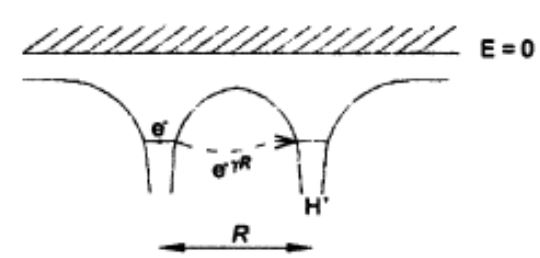
\includegraphics[width=0.5\linewidth]{res_recharge.jpg}
	\end{center}
	\caption{Схема туннелирования атомного электрона (внизу) при резонансной перезарядке}
	\label{fig:charge_exchange}
\end{figure}

\uline{Нерезонансная перезарядка} состоит в передаче электрона от одного ядра к другому в случае неидентичных ядер с разными энергиями связи электрона на каждом из них.

Особый случай соответствует перезарядке атома на многозарядном ионе, потенциал ионизации которого намного превосходит потенциал ионизации исходного атома. Здесь атомный электрон переходит в густой спектр высоковозбужденных состояний многозарядного иона, для которых энергия связи близка к энергии связи в исходном атоме. Сечение такой перезарядки $\sigma_{exchange} \sim Zn^4$, где $Z$ -- заряд иона, $n$ -- номер орбиты~\cite{astap}.

\subsubsection{Прилипание}

Процесс прилипания дополнительного электрона к изначально нейтральным атомам или молекулам достаточно важен. Например, это канал потерь электронов, который может быть использован. Большие потери электронов в газах с активными электроотрицательными [свойство притягивать к себе дополнительные электроны] добавками затрудняют развитие в них электронной лавины, что повышает напряжение пробоя. Это используют в счётчиках Гейгера, в которых быстрые ядерные и атомные частицы регистрируются благодаря производимой ими ионизации. После пролета частицы необходимо возможно скорее устранить электроны, чтобы подготовить прибор для регистрации нового разрядного импульса.
 
Механизмы прилипания электронов к нейтральным частицам во многом похожи на механизмы рекомбинации электронов с положительными ионами: фотозахват, тройные столкновения, диссоциативное прилипание.
 
Термодинамически равновесные плотности отрицательных ионов не зависят от механизмов образования и разрушения ионов и определяются уравнением Саха, в котором по смыслу роль положительных ионов играют нейтральные частицы, а роль атомов и молекул — отрицательные ионы.

\uline{Прилипание в результате фотозахвата.} Захват электронов атомами водорода с испусканием кванта имеет важное значение в излучении звезд, но практически неважен в исследовании газового разряда.

\uline{Прилипание в результате тройных столкновений.} Затрат энергии для этого процесса не требуется, и потому он легко идет при комнатной температуре электронов и в очень слабых полях. Малые (но не чрезмерно) энергии электронов для него даже предпочтительнее. В некоторых газах, в частности -- в воздухе, прилипание в тройных столкновениях является главным механизмом потерь медленных электронов.

\begin{equation*}
	e + A + A \leftrightarrow A^{-} + A
\end{equation*}

Фактически подобные процессы протекают многоступенчатым путем. Например, для воздуха электрон вначале в парном столкновении захватывается молекулой $O_2$ в автоионизационное состояние. При этом сверхвозбужденными оказываются не электронные степени свободы, как при безызлучательном захвате электрона положительным ионом, а молекулярные колебания. В последующих соударениях с молекулами сверхвозбужденные ионы, которые не успели совершить автоионизационный распад, стабилизируются благодаря ударной дезактивации (``тушению''). Иногда столкновения вызываются действием поляризационных сил, и молекула просто отбирает у иона часть колебательной энергии: иногда наряду с передачей энергии происходит резонансная перезарядка. С молекулами кислорода последний вариант случается даже чаще.

\uline{Диссоциативное прилипание.} По данному механизму образовываются в плазменном объёме отрицательные ионы водорода. Для них он происходит в две стадии: сначала ``горячий'' электрон ($\varepsilon \approx 30-100$ эВ) возбуждает высокие колебательные состояния молекулы водорода, а потом к ней прилипает холодный ($\varepsilon \sim 1$ эв) электрон, квазимолекула распадется на искомый ион $H^{-}$ и атом $H$.

Процессы диссоциативного прилипания имеют резонансный характер. В зависимости от энергии электрона наблюдаются резко выраженные максимумы сечений~\cite{raizer}. При повышении температуры газа сечение диссоциативного прилипания возрастает, а энергетический порог реакций понижается, но так происходит лишь после некоторого повышения температуры.

\subsubsection{Возбуждение и диссоциация молекул электронным ударом}

\uline{Возбуждение в результате соударения с электроном.} Три основных типа атомно-молекулярных частот: электронные с энергиями порядка нескольких эВ, колебательные с энергиями порядка долей эВ, вращательные с энергиями порядка сотых долей эВ~\cite{astap}.

Возбуждения \uline{электронных состояний} существенным образом влияют на скорость развития электронной лавины во многих случаях пробоя газов. Они составляют первый этап процесса ступенчатой ионизации в газе и вообще являются главным механизмом появления возбужденных атомов и молекул в плазме. Возбуждение атомов и молекул в значительной степени обусловливает свечение разрядной плазмы~\cite{raizer}.

В отличие от ударной ионизации, когда атомный электрон возбуждается в непрерывный энергетический спектр, соответствующий инфинитному движению, в случае возбуждения атомный электрон переходит в состояние дискретного спектра, то есть (в рамках классической картины) на другую атомную орбиту с большей энергией. Это явление ответственно за излучение фотонов в плазме, возникающее в результате обратного перехода атомного электрона из возбужденного состояния в основное~\cite{astap}.

\begin{equation*}
	e + A \rightarrow A^{*} + e
\end{equation*}

Атом при взаимодействии с электромагнитным полем ведёт себя как набор осцилляторов, которые ставятся в соответствие паре энергетических уровней $E_i$ и $E_j$ атомного спектра причём собственные частоты этих осцилляторов равны собственной частоте перехода $\omega_{i,j}=\frac{E_j-E_i}{\hbar}$ (для дипольно-разрешённых переходов).

Дипольно-запрещённые переходы бывают двух типов: без изменения спина атома (дипольный момент перехода отсутствует из-за невыполнения правил отбора по орбитальному квантовому числу $L$, переход осуществляется за счёт прямого кулоновского взаимодействия) и переходы с изменением атомного спина (в этом случае возбуждение атома происходит за счет обменного взаимодействия между налетающим и атомным электроном)~\cite{astap}.

Среди возбужденных атомов и молекул выделяются метастабильные частицы. Из метастабильных состояний запрещен, т. е. имеет чрезвычайно малую вероятность, самопроизвольный переход в нижнее энергетическое состояние, сопровождающийся излучением кванта. Следовательно, в таких состояниях частица может жить долго, до тех пор, пока она не дезактивируется ударом другой частицы, электрона или атома и не перейдетв более высокое состояние или не ионизируется. В сильно разреженных газах это время может быть весьма большим. Времена жизни метастабильных состояний по отношению к высвечиванию превышают $10^{-4}$ с и достигают в некоторых случаях секунд, тогда как обычные возбужденные атомы и молекулы высвечиваются через $10^{-9}-10^{-7}$ с (если не будут до этого дезактивированы ударом). Особенно велика роль метастабильных частиц для процесса ступенчатой ионизации, так как они живут долго и поэтому ``с легкостью ожидают'' ионизирующего удара.

Самый нижний из неметастабильных уровней называют резонансным. Возможен такой процесс: атом излучает квант света, возвращаясь в основное состояние. Этот квант с большой вероятностью поглощается соседним атомом, поскольку происходит резонансное поглощение, и переводит его на тот же самый резонансный уровень. Второй атом излучает квант и т. д. Так происходят блуждание (диффузия) резонансного излучения и периодическое появление и исчезновение резонансно возбужденных атомов. Процессу препятствует дезактивация (тушение) резонансно возбужденных атомов.

Эффективное сечение возбуждения электронного состояния $\sigma_{exc}(\varepsilon)$ называют иногда функцией возбуждения. В зависимости от энергии электрона это сечение ведет себя в качественном отношении так же, как сечение ионизации, только максимум располагается ближе к порогу. Этот процесс -- сугубо квантовый.

Возбуждение \uline{колебательных частот} играет существенную роль в разрядах, происходящих в молекулярных газах, будучи главным механизмом передачи энергии от электронов молекулам. Можно провести аналогию с ударами по двум шарам, соединённых пружиной. Иногда процесс идёт через промежуточное состояние (отрицательный молекулярный ион).

При рассмотрении возбуждения \uline{вращательных частот} можно провести аналогию с ударами по гантели (два жёстко соединённые шара). Вообще говоря, роль возбуждения и дезактивации молекулярных вращений электронным ударом для разрядных процессов не очень существенна. В атомарных газах этого процесса просто нет, а в молекулярных обмен вращательной энергией значительно уступает обмену колебательной, так как соответствующие порции энергии -- колебательные кванты -- на несколько порядков больше~\cite{raizer}.

\uline{Диссоциация молекул в результате соударения с электроном.} Удары достаточно энергичных электронов могут приводить и к диссоциации молекул. Этот неупругий процесс, как правило, не оказывает существенного влияния на энергетический баланс электронов в разряде, уступая в этом отношении возбуждению колебательных уровней молекул. Но в определенных условиях диссоциация молекул имеет большое непосредственное значение, будучи начальным этапом в цепочке последующих химических превращений. Для многих плазмохимических реакций ``узким местом'', определяющим скорость всего процесса, является образование из молекул атомов и свободных радикалов, которые потом уже достаточно быстро реагируют с другими компонентами. Прохождению этого этапа и способствует диссоциация молекул ударами электронов в разряде. Вероятность прямого разбиения молекулы за счет кинетической энергии электрона очень мала. Диссоциация идет двухступенчатым путем, но в отличие от возбуждения колебаний не через захват электрона, а через возбуждение электронных или электронно-колебательных состояний молекулы с последующим распадом возбужденной молекулы на атомы. Вклад в диссоциацию дает возбуждение нескольких подходящих уровней молекулы, соответствующих нестабильным состояниям, так что процесс идет по нескольким каналам. Процесс носит пороговый характер, порог определяется не потенциалом диссоциации, а потенциалом возбуждения низшего нестабильного электронного состояния~\cite{raizer}.

\section{Физическая кинетика}
\label{sec.3}

Макроскопические уравнения плазмы являются уравнениями переноса в том смысле, что они описывают поток импульса, энергии и т. д. Однако термин «явления переноса» употребляется в физике плазмы обычно для обозначения свойств плазмы, связанных со столкновительными эффектами, т. е. таких свойств, как электропроводность, теплопроводность, диффузия частиц поперек или вдоль магнитного поля и т. д. Во многих плазменных задачах поведение плазмы определяется влиянием нейтральных атомов или молекул. Например, диффузия электронов в редкой низкотемпературной частично ионизованной плазме определяется главным образом столкновениями электронов с нейтралами. Кроме того, разнообразные процессы в плазме происходят в результате ионизации при столкновениях и электрон-ионной рекомбинации. В проблеме явлений переноса в плазме имеются два аспекта. Первый из них связан с вычислением различных коэффициентов переноса на основании соответствующего статистического описания и анализа механизмов, приводящих к этим явлениям. Другой аспект состоит в том, чтобы с помощью полученных коэффициентов рассчитать ожидаемую макроскопическую картину поведения плазмы при данных начальных и граничных условиях~\cite{kroll}.

\subsection{Уравнения Больцмана и Власова, интеграл столкновений, время максвеллизации и скорость выравнивания температур различных компонент плазмы}

Наиболее подробное описание плазмы дается набором изменяющихся во времени координат и скоростей всех частиц. Для реальной плазмы достичь такого уровня описания невозможно. Предлагается использовать формализм теории вероятностей и статистической физики\Tokman.

Поскольку в течение промежутков времени, меньших времени электрон-ионных столкновений, поведение электронов и ионов может сильно различаться, обычно необходимо определять для частиц каждого сорта $\alpha$ свою функцию распределения $f_\alpha(\vec{r_\alpha}, \vec{v_\alpha})$.

\subsubsection{Ввод понятия функции распределения}

Рассмотрим ящик классических частиц объёмом $V$, в котором $N$ частиц: $\vec{r_1}, \vec{r_1},\ldots,\vec{r_N}$. 

Тогда плотность вероятности найти первую частицу в $\vec{r_1}$, вторую -- в $\vec{r_2}$ и т.д. [без учёта движения частиц=скорости] вводится как $\omega(\vec{r_1}, \vec{r_1},\ldots,\vec{r_N})$ (нормирована на единицу: $\prod\limits_{j} \int\limits_{V} d^3r_j \omega = 1$).

Число частиц в объёме $\Delta V$ вводится как интеграл от $n(\vec{r})=\sum\limits_{j}\delta(\vec{r}-\vec{r_j})$ -- концентрации:

\begin{equation*}
	\Delta N = \int\limits_{\Delta V} n(\vec{r}) d^3r,
\end{equation*}

Введём для концентрации выражение через усреднение по вероятностному распределению:

\begin{equation*}
	n(\vec{r}) = \prod\limits_{j}\int\limits_{V}d^3r_j \sum\limits_{j} \delta(\vec{r}-\vec{r_j})\omega(\vec{r_1}, \vec{r_2}, \vec{r_N}) = \sum\limits_j \omega_{1j}(\vec{r})\delta(\vec{r}-\vec{r_j}),
\end{equation*}

где $\omega_1(\vec{r_j}) = \prod\limits_{j'\neq j}\omega(\vec{r_1} \ldots \vec{r_j} \ldots \vec{r_N}) d^3r_{j'}$ -- вероятность найти первую [если одинаковые: одну] частицу в $\vec{r_j}$.

Для случая одинаковых частиц (т.е. частиц одного сорта) $\omega_1$ -- одинаковые. Тогда $n(\vec{r}) = N\cdot\omega_1(\vec{r})$.

\begin{quotation}
	[Оффтоп] Вероятность нахождения первой из одинаковых частиц в $\vec{r}$, а второй -- в $\vec{r'}$: $\omega_2(\vec{r}, \vec{r'}) = \omega_1(\vec{r})\omega_{1}(\vec{r'})$.
\end{quotation}

Рассмотрим 2 сорта частиц $\alpha$ и $\beta$. Для них плотность вероятности вводится так: \newline $\omega_{\alpha\beta}(\overrightarrow{r_{1\alpha}}\ldots\overrightarrow{r_{N\alpha}},\overrightarrow{r_{1\beta}}\ldots\overrightarrow{r_{N\beta}})$, причём вероятность найти одну частицу сорта $\alpha$ в заданной точке $\omega_{1\alpha}$ получается интегрированием по всем $\vec{r_\beta}$ и по всем $\vec{r_\alpha}$, кроме одной.

Введём плотность вероятности с учётом того, что частицы движутся: $\overrightarrow{r_{\alpha, \beta}}\Rightarrow\overrightarrow{r_{\alpha, \beta}};\overrightarrow{v_{\alpha, \beta}}$ (полный набор координат частицы описывает её нахождение в 6D пространстве координат/скоростей). Теперь имеет смысл оперировать понятием вероятности найти одну частицу в заданной точке с заданной скоростью $\omega_{1\alpha}(\overrightarrow{r_\alpha}, \overrightarrow{v_\alpha})$.

\uline{Функция распределения} [ФР; часто используется сокращение ФРЭЭ -- функция распределения электронов по энергиям] частиц сорта $\alpha$ [по скоростям и координатам] вводится так:

\begin{equation} \label{eq:distribution_func}
	f_\alpha(\overrightarrow{r_\alpha}, \overrightarrow{v_\alpha}) = n_\alpha\cdot\omega_{1\alpha}(\overrightarrow{r_\alpha}, \overrightarrow{v_\alpha})
\end{equation}

[Физ. смысл] ФР есть плотность частиц в фазовом пространстве. Интеграл от неё по скоростям есть концентрация частиц, по скоростям и координатам -- полное число частиц выбранного сорта~\cite{kotelnikov}.

\subsubsection{Вычисление макрохарактеристик плазмы с использованием ФР}

Концентрация частиц:

\begin{equation*}
	n_\alpha(\vec{r}) = \int\limits_{\infty}f_\alpha d^3v_\alpha
\end{equation*}

Средний поток частиц:

\begin{equation*}
	\Pi_\alpha(\vec{r}) =	\int\limits_{\infty}\overrightarrow{v_\alpha}f_\alpha d^3v_\alpha
\end{equation*}

Средний импульс:

\begin{equation*}
	p_\alpha(\vec{r}) = \int\limits_{\infty}m_\alpha\overrightarrow{v_\alpha}f_\alpha d^3v_\alpha
\end{equation*}

Средняя кинетическая энергия:

\begin{equation*}
	K_\alpha(\vec{r}) = \int\limits_{\infty}\frac{m_\alpha\overrightarrow{v_\alpha}}{2}f_\alpha d^3v_\alpha \xrightarrow{\text{если не зависит от $\vec{r}$}} <K_\alpha>n_\alpha
\end{equation*}

\subsubsection{Двухчастичная ФР}

Собственно, имеет вид $f_{\alpha\beta}(\overrightarrow{r_\alpha}, \overrightarrow{r_\beta}, \overrightarrow{v_\alpha}, \overrightarrow{v_\beta}) = n_\alpha n_\beta \widetilde{f_{\alpha\beta}}(\overrightarrow{v_\alpha}, \overrightarrow{v_\beta})$. Для независимых (невзаимодействующих)

\begin{equation} \label{eq:Boltzmann_relation}
	f_{\alpha\beta} = f_\alpha f_\beta
\end{equation}

\begin{quotation}
	Последнее выражение -- \uline{приближение Больцмана}\Tokman. Если написать последовательно кинетические уравнения для $N, N-1, \ldots, 1$-частичных функций распределения, получится т.н. цепочка уравнений Боголюбова. Это приближение позволяет её замкнуть и решить. 
\end{quotation}
	
\begin{equation*}
	\int\limits_{\infty}f_{\alpha\beta}(\overrightarrow{r_\alpha}, \overrightarrow{r_\beta}, \overrightarrow{v_\alpha}, \overrightarrow{r_\beta})d^3v_\alpha d^3v_\beta = n_{\alpha\beta}(\overrightarrow{r_\alpha}, \overrightarrow{r_\beta}) \xrightarrow{\text{независимые}} n(\overrightarrow{r_\alpha}) n(\overrightarrow{r_\beta})
\end{equation*}
	
Разница $n_{\alpha\beta}-n_\alpha n_\beta$ перестаёт быть малой на радиусе корреляции (дебаевский радиус), однако в первом приближении ФР расщепляется.

\subsubsection{Вывод уравнения Больцмана}

Рассмотрим частицы одного сорта $f(\vec{r}, \vec{v}, t)$ при наличии внешней силы $\vec{F}(\vec{r}, t)$, где $\vec{r} = \vec{r}(t)$, $\vec{v} = \vec{v}(t)$.
	
У системы уравнений движения есть два векторных интеграла движения, сохраняющихся на решениях уравнений: $\vec{r_0} = \vec{r_0}(t, \vec{v}, \vec{r})$; $\vec{v_0} = \vec{v_0}(t, \vec{v}, \vec{r})$ В начальный момент было $f(\overrightarrow{r_0}, \overrightarrow{v_0})$. Значит, [т.к. нормировка = общее число частиц сохраняется]: 

\begin{equation*}
	f(\vec{r}, \vec{v}, t) = f(\overrightarrow{r_0}(t, \vec{v}, \vec{r}), \overrightarrow{v_0}(t, \vec{v}, \vec{r})) \cdot \abs{\frac{D(\vec{r}, \vec{v})}{D(\overrightarrow{v_0}, \overrightarrow{r_0})}} = f(\overrightarrow{r_0}(t, \vec{v}, \vec{r}), \overrightarrow{v_0}(t, \vec{v}, \vec{r})) \cdot J
\end{equation*}
	
Мы рассматриваем частицы под воздействием полей, а столкновения и трения не рассматриваем, то система консервативная и по теореме Лиувилля якобиан $J=1$. 
$f(\overrightarrow{r_0}(t, \vec{v}, \vec{r}), \overrightarrow{v_0}(t, \vec{v}, \vec{r}))$ -- интеграл движения как функция от интегралов; значит, $f(\vec{r}, \vec{v}, t)$ -- тоже.

Значит, \uline{кинетическое уравнение в бесстолкновительном приближении}/\newline\uline{бесстолкновительное уравнение Больцмана}/\uline{уравнение Лиувилля}

\begin{equation} \label{eq:Liouville_eq}
	\frac{df}{dt} = \frac{\partial f}{\partial t} + \frac{d\vec{r}}{dt}\frac{\partial f}{\partial \vec{r}}+ \frac{\vec{F}}{m}\frac{\partial f}{\partial \vec{v}} = 0
\end{equation}

Важно: здесь $F$ -- сила не трения, а подобная силе Лоренца, чтобы работала теорема Лиувилля.

Если в системе есть соударения, то справа надо дописать ещё столкновительный член $St$ (он же -- \uline{интеграл столкновений}, оператор соударений, часто обозначается как $\frac{\partial f}{\partial t}\bigg|_\text{столк}$). Строгий вывод: последовательное интегрирование уравнений Лиувилля (цепочка уравнений Боголюбова). Интеграл столкновений по физическому смыслу есть скорость изменения функции распределения в результате столкновений. Больцмановский подход предполагает рассмотрение только парных столкновений и замыкание системы (см. выше приближение Больцмана~\ref{eq:Boltzmann_relation}).

\uline{Уравнение Больцмана}:

\begin{equation} \label{eq:Boltzmann_eq}
	\frac{df}{dt} = \frac{\partial f}{\partial t} + \frac{d\vec{r}}{dt}\frac{\partial f}{\partial \vec{r}}+ \frac{\vec{F}}{m}\frac{\partial f}{\partial \vec{v}} = St
\end{equation}

Важно: Фазовое пятно из-за столкновений не сохраняется.

Важно: Хотя кинетическое уравнение Больцмана не дает точного описания эволюции распределения в результате столкновений в полностью ионизованной плазме, его можно использовать для вычисления коэффициентов переноса
в слабоионизованной плазме, где превалируют упругие столкновения электронов с нейтральными частицами~\cite{kroll}.

Свойства: 1. При интегрировании кинетического уравнения по скорости получаем:

\begin{equation*}
	\frac{\partial n}{\partial t} + div(n\vec{v}) = \int\limits_{\infty}d^3v\cdot St
\end{equation*}

Из уравнения непрерывности следует, что для любого интеграла столкновений 

\begin{equation*}
	\int\limits_{\infty}d^3v\cdot St = 0
\end{equation*}

2. При равновесной $f=f_0$ интеграл столкновений зануляется: $St = 0$
	
\subsubsection{Время максвеллизации и скорость выравнивания температур различных компонент плазмы} \label{subsec: maxwellization_time}

Существуют разные подходы к конкретному виду интеграла столкновений. Стоит точно назвать интегралы соударений в формах Больцмана, Фоккера-Планка и БГК. Более подробно они рассмотрены в первом билете дополнительной программы~(\ref{subsec:collision_terms}).

Существует приближение, связанное с введением времени свободного пробега (т.н. $\tau$-приближение, а уравнение Больцмана с ним называется модифицированным). В этом методе больцмановский интеграл столкновений заменяют следующим выражением~\cite{kroll}:

\begin{equation*}
	\frac{\partial f}{\partial t}\bigg|_\text{столк} = \frac{f_0-f(\vec{r}, \vec{v}, t)}{\tau(v)}\approx-\frac{f_0-f(\vec{r}, \vec{v}, t)}{\tau},
\end{equation*}

где $\tau$ -- постоянное время свободного пробега. Уравнение Больцмана в таком виде иногда называют \uline{моделью Крука}.

Данный подход отражает представление о том, что любое распределение
релаксирует к равновесному распределению $f_{\alpha 0}$ за счет столкновений и что существует некоторое характерное время (в общем случае зависящее от скорости) между столкновениями с передачей импульса -- \uline{время максвеллизации}.

Применимость:

1. [Закон сохранения числа частиц] Равновесная функция $f_0$ имеет вид распределения Максвелла-Больцмана:

\begin{equation*}
	f_{\alpha 0} = \frac{n_\alpha(\vec{x}, t)}{\overline{n_\alpha}} \left( \frac{m_\alpha}{2\pi \varkappa T_\alpha}\right)^{3/2}e^{-m_\alpha v^2/(2\varkappa T_\alpha)}, 
\end{equation*}

\begin{equation*}
	\frac{n_\alpha(\vec{x}, t)}{\overline{n_\alpha}} \equiv \int f_\alpha (\vec{r}, \vec{v}, t) d\vec{v},
\end{equation*}

где $\overline{n_\alpha}$ -- отношение полного числа частиц к полному объёму системы.

2. Интеграл столкновений видоизменяет распределение таким
образом, что средняя скорость обращается в нуль. Это удачное приближение для столкновений электронов с нейтральными частицами, а, значит, слабоионизованной плазмы. Подобный подход называется моделью Лоренца.

Замена $\tau(v)$ на $\tau$ является точной в случае короткодействующей силы. Выбор времени т, не зависящего от функции распределения $f_\alpha$, который линеаризует больцмановский интеграл
столкновений, возможен только тогда, когда отсутствуют столкновения
между частицами того же распределения.

3. Член $\frac{f}{\tau}$ описывает уход частиц, распределенных согласно
$f(\vec{r}, \vec{v}, t)$, за счет рассеяния из элемента $d\vec{v}$. Это напоминает процесс поглощения, поскольку все частицы, первоначально находившиеся в элементе $d\vec{v}$, исчезают из данного элемента после рассеяния. Второй член интеграла столкновений описывает приход частиц в элемент $d\vec{v}$ за счет рассеяния;
ему трудно найти аналогию в исходном уравнении Больцмана. Форма $\frac{f_0}{\tau}$ предполагает, что после каждого столкновения испускаются частицы с максвелловским распределением и локальной плотностью $n(\vec{r}, t)$.

\uline{Скорость выравнивания температур различных компонент в плазме}

\subsubsection{Уравнение Власова}

Случай бесстолкновительной плазмы во внешних э/м полях:

\begin{equation} \label{eq:Vlasov_eq_main}
	\frac{\partial f_\alpha}{\partial t}+\vec{v}\frac{\partial f_\alpha}{\partial \vec{r}}+e_\alpha\left(\vec{E}+
	\frac{1}{c}\left[\vec{v}\times\vec{B}\right]\right)\frac{\partial f_\alpha}{\partial \vec{p}}=0
\end{equation}

При рассмотрении плазмы в э/м полях возникают сложности при использовании больцмановского подхода (ур.~\ref{eq:Boltzmann_eq}), а именно: рассматриваются только парные столкновения, сечения которых при кулоновском взаимодействии, строго говоря, расходятся, т.к. оно имеет дальнодействующий характер и одна частица взаимодействует не с одной, а с совокупностью частиц. Соответственно и то эффективное поле, которым можно описать
это взаимодействие, создаётся большим числом частиц, т. е. имеет
макроскопический характер. Тем самым весь процесс приобретает
макроскопически достоверный, а не случайный характер. Есть и другие причины (см, например, [Вики],~\cite{kotelnikov}).

Этому случайному характеру формально отвечает представление точных
микроскопических значений электрического и магнитного полей, действующих на некоторую частицу в плазме, в виде~\cite{kotelnikov}:

\begin{align*}
	\vec{E} = \langle\vec{E}\rangle+\vec{e};\\
	\vec{B} = \langle\vec{B}\rangle+\vec{b},	
\end{align*}

где $\langle\vec{E}\rangle$ и $\langle\vec{B}\rangle$ -- некие средние поля, создаваемые ``средней'' плотностью заряда и ``средним'' током в плазме, а микрополя $\vec{e}$ и $\vec{b}$ представляют собой мелкомасштабные флуктуации полей, отвечающие
столкновениям частиц. Переобозначим $\langle\vec{E}\rangle$ и $\langle\vec{B}\rangle$ как $\vec{E}$ и $\vec{B}$. Условие на них -- уравнения Максвелла:

\begin{align} \label{eq:Vlasov_eq_Maxwell}
	rot\vec{E} = -\frac{1}{c}\frac{\partial \vec{B}}{\partial t},\;div\vec{B}=0;\\
	rot\vec{B} = \frac{1}{c}\frac{\partial \vec{E}}{\partial t}+\frac{4\pi}{c}\vec{j},\;div\vec{E}=4\pi\rho;
\end{align}

где плотности заряда и тока выражаются через саму ФР:

\begin{align} \label{eq:Vlasov_eq_extra}
	\rho = \sum\limits_{\alpha}\int e_\alpha f_\alpha d^3p, \\
	\vec{j} = \sum\limits_{\alpha}\int e_\alpha \vec{v}f_\alpha d^3p;
\end{align}

Самосогласованная система уравнений~(\ref{eq:Vlasov_eq_main}, \ref{eq:Vlasov_eq_Maxwell}, \ref{eq:Vlasov_eq_extra}) с т.н. самосогласованными полями $\vec{E}$ и $\vec{B}$ -- уравнения Власова (или просто~(\ref{eq:Vlasov_eq_main}) -- \uline{уравнение Власова}).

\subsection{Явления переноса в плазме, электропроводность, диффузия и теплопроводность частиц при наличии и отсутствии магнитного поля}

Эволюция плазмы заключается в направлении выравнивания её параметров между различными частями пространства за счёт процессов переноса, которые приводят к перераспределению плотности, импульса и энергии между различными областями плазмы. Процессами переноса называют в совокупности диффузию, теплопроводность и вязкость. В замкнутой системе они ведут к установлению полного термодинамического равновесия. Они обусловлены кулоновскими столкновениями, но идут ещё медленнее, нежели локальное выравнивание температуры ионов и электронов~\cite{kotelnikov}.

\subsubsection{При отсутствии магнитного поля}

Рассмотрим электроны с независимой от времени ФРЭЭ в постоянном однородном электрическом поле. Пусть $f = f_0+\delta f$

\begin{equation*}
	-\frac{e\vec{E}}{m}\frac{\partial f}{\partial \vec{v}} = \frac{f_0-f}{\tau} = -\frac{\delta f}{\tau}
\end{equation*}

\begin{equation*}
	\delta f = \tau \frac{e\vec{E}}{m} \frac{\partial f_0}{\partial \vec{v}}
\end{equation*}

Тогда плотность тока равна:

\begin{equation*}
	\vec{j} = -e\int\limits_{\infty}d^3v\cdot \vec{v} \delta f = -\frac{e^2\tau}{m} \vec{E} \left(vf_0\bigg|_{-\infty}^{+\infty}-\int\limits_{\infty}d^3v\cdot f_0\right) = -\frac{e^2\tau}{m} \vec{E} (0-n) \equiv \sigma \vec{E},
\end{equation*}

где $\sigma = \frac{e^2n\tau}{m}$ -- \uline{электропроводность}.

Применимость:

\begin{equation*}
	f_0 \gg \delta f \sim \frac{eE\tau}{m}\frac{f_0}{v_T} \leftrightarrow v_T \gg \frac{eE\tau}{m} = a\cdot \tau
\end{equation*}

Скорость, которую между столкновениями успевает набрать частица, много меньше тепловой.

Если температура плазмы неоднородна, то в процессе такого
диффузионного движения происходит перенос тепла, описываемый
обычным уравнением теплопроводности с коэффициентом температуропроводности, который по физическому смыслу получается
умножением коэффициента диффузии на теплоемкость~\cite{arzimovich}.

Пусть есть в плазме с максвелловской ФР ($f_0 = n\sqrt{\frac{m}{2\pi T(x)}}e^{-\frac{mv^2}{2T(x)}}$) неоднородность температуры с характерной длиной $L_{eff} = \frac{T}{T_x^{'}} \gg \tau v_T$. Из кинетического уравнения с интегралом столкновений в форме БГК следует:

\begin{equation*}
	V_x\frac{\partial f_0}{\partial x} = \frac{f_0-f}{\tau} = -\frac{\delta f}{\tau}
\end{equation*}

\begin{equation*}
	\delta f = -\tau v_x \frac{\partial f_0}{\partial x} = -\tau v_x f_0 \left(-\frac{1}{2T(x)}+\frac{mv^2}{T(x)^2}\right)T_x^{'}
\end{equation*}

Тогда поток тепла в направлении $x$:

\begin{equation*}
	g_x = \int\limits_{\infty}d^3v\cdot v_x\frac{mv^2}{2}\delta f = -3\pi n \frac{T\tau}{m} \frac{\partial T}{\partial x} \equiv -\varkappa \frac{\partial T}{\partial x},
\end{equation*}

где $\varkappa = 3\pi n \frac{T\tau}{m}$ -- \uline{теплопроводность}; $\frac{1}{\tau} = \frac{1}{\nu_{ee}+\nu_{ei}}$

\subsubsection{При наличии магнитного поля}

\begin{equation*}
	\frac{\partial f_\alpha}{\partial t} + (\vec{v}\nabla)f_\alpha+\frac{e_\alpha}{m_\alpha}\left\{\vec{E}+\frac{1}{c}\left[\vec{V}\times\vec{B}\right]\right\}\frac{\partial f_\alpha}{\partial \vec{v}} = St\left\{f_\alpha\right\}
\end{equation*}

Нерелятивистский случай: можно пренебречь силой Лоренца, поэтому здесь магнитное поле -- стороннее ($\abs{\vec{B}} \gg \abs{\vec{E}}$).

Влияние электрического поля: ``кулоновское обрезание на дебаевском радиусе'': $\rho_{max} = r_d$. 

Влияние магнитного поля: : ``ларморовское обрезание на дебаевском радиусе'':
$\rho_{max} = r_B$\Tokman. 

Получается, что при $r_B \gg r_d$ влиянием магнитного поля на (кулоновские) столкновения можно пренебречь: $r_b=\frac{v_T}{\omega_B} \gg r_d=\frac{v_T}{\omega_{p}} \leftrightarrow \omega_B^2 \ll \omega_{p}^2$.

Для электронов не выполняется в типичной плазменной ловушке. Для электронов и ионов может выполнять. Если так, то к частоте столкновений добавляется слагаемое $\abs{ln\frac{\omega_{Be}}{\omega_{pe}}}$. Как правило, $L \simeq 10 \gg \abs{ln\frac{\omega_{Be}}{\omega_{pe}}}$.

Если поле $\vec{E}$ -- большое, то осцилляторный радиус $\tilde{r}$ играет ту же роль, что и $r_B$. При наличии магнитного поля уже нельзя сказать, что классическое и квантовое решения задачи совпадают всегда. В случае больших полей приходится честно решать уравнение Шрёдингера.

\paragraph{Диффузия}

Движение каждой заряженной частицы в плазме носит случайный диффузионный характер, однако макроскопический смысл имеется лишь при рассеянии частиц друг на друге\cite{arzimovich}.

\begin{quotation}
	Здесь рассматривается случай наличия магнитного поля. Для его отсутствия подвижность -- не тензор, а скаляр, равный продольной (по отношению к магнитному полю) компоненте тензора. Его вывод аналогичен, поэтому опустим его.
\end{quotation}

Рассмотрим уравнения МГД для магнитно-активной (постоянное магнитное поле) плазме\Tokman. 

\begin{equation*}
	m_\alpha\frac{d\overrightarrow{u_\alpha}}{dt}=e_\alpha\vec{E}+\frac{e_\alpha}{c}\left[\overrightarrow{u_\alpha}\times\vec{B}\right]-\frac{1}{N_\alpha}\nabla\left(N_\alpha T_\alpha\right)- m_\alpha\sum\limits_{\beta}\nu_{\alpha\beta}^t\left(\overrightarrow{u_\alpha}-\overrightarrow{u_\beta}\right),
\end{equation*}

где $\nu_{\alpha\beta}^t$ -- транспортная частота = характерная частота потери импульса, а $\beta$ -- все сорта частиц, с которыми соударяются частицы сорта $\alpha$. Здесь $T_\alpha=const$ -- для электронов обосновывается стабилизацией за счёт быстрого движения вдоль силовых линий.

Условие применимости диффузного описания: масштаб неоднородностей (всех) $L \gg \lambda_\alpha$ -- длины свободного пробега.

Рассмотрим стационар (поля постоянные, однородная температура, рассматривается только линейный отклик, сорт $\beta$ -- один [например, остаточные нейтралы. Случай $e$ и $i$ -- особый]):

\begin{equation*}
	\nu_\alpha \overrightarrow{u_\alpha} + \left[\overrightarrow{\omega_{B\alpha}}\times \overrightarrow{u_\alpha}\right] = \frac{e_\alpha}{m_\alpha}\vec{E}-\frac{T_\alpha}{m_\alpha}\frac{\nabla N_\alpha}{N_\alpha}
\end{equation*}

Часто вводят $\left(\frac{e_\alpha}{m_\alpha}\vec{E}\right)_{eff} = \frac{e_\alpha}{m_\alpha}\vec{E}-\frac{T_\alpha}{m_\alpha}\frac{\nabla N_\alpha}{N_\alpha}$, тогда решение есть $\overrightarrow{u_\alpha} = \overrightarrow{u_\alpha} (\overrightarrow{E_{eff}})$. Решение известно (см. вывод уравнения движений в магнитных полях~\ref{eq}).

Решать надо вместе с уравнением непрерывности:

\begin{equation*}
	\frac{\partial N_\alpha}{\partial t} + div(N_\alpha\overrightarrow{u_\alpha}) = 0
\end{equation*}

Фактическое решение:

\begin{equation*}
	\overrightarrow{u_\alpha} = \widehat{b_\alpha} \overrightarrow{E_{eff}} = \widehat{b_\alpha} \left(\vec{E}-\frac{T_\alpha}{e_\alpha}\frac{\nabla N_\alpha}{N_\alpha}\right),
\end{equation*}

где $\widehat{b_\alpha}$ -- тензор \uline{подвижности}. А $\widehat{D} = \frac{T_\alpha}{e_\alpha}\widehat{b_\alpha}$ -- коэффициент \uline{диффузии}.

\begin{equation*}
	b^\alpha_{ij} = 
	\begin{pmatrix}
		b_{\perp\alpha} & b_{d\alpha} & 0 \\
		-b_{d\alpha} & b_{\perp\alpha} & 0 \\
		0 & 0 & b_{\parallel\alpha}
	\end{pmatrix},
\end{equation*}

где $b_{\perp\alpha} = \frac{e_\alpha}{m_\alpha}\frac{\nu_\alpha}{\nu_\alpha^2+\omega_{B\alpha}^2}$; $b_{d\alpha} = \frac{e_\alpha}{m_\alpha}\frac{\omega_{B\alpha}}{\nu_\alpha^2+\omega_{B\alpha}^2}$; а коэффициент диффузии вдоль магнитного поля равен $b_{\parallel\alpha} = \frac{e_\alpha}{m_\alpha\nu_\alpha}$ -- как без магнитного поля.

\begin{quotation}
	Отсюда всплывает дрейф: скорость поперёк магнитного поля для частицы сорта $\alpha$: $\overrightarrow{u_{\perp\alpha}} = c\frac{\vec{E}\times\vec{B}}{B^2}\sim e_\alpha^2$ -- не зависит от знака заряда.
\end{quotation}

Коэффициент диффузии разный для разных сортов частиц -- возникает эффект \uline{амбиполярной диффузии} (см. раздел ~\ref{subsec}). Его свойство: суммарный электрический ток электронов и ионов в направлении градиента плотности 
равен нулю, обеспечивая сохранение квазинейтральности плазмы.

По порядку величины коэффициент диффузии примерно равен квадрату ларморовского радиуса электрона, делённому на средний интервал времени между двумя последовательными столкновениями электрона с ионами: $D_e\sim\frac{r_{Be}^2}{\tau_{ei}}\sim\frac{T_e}{m_e\omega_{Be}\tau_{ei}}$, т.к. при каждом столкновении с ионом, сопровождающемся рассеянием на угол порядка $\pi/2$, электрон смещается случайным образом на расстояние порядка ларморовского радиуса. В то же время $D_i\sim\frac{T_i/Z}{m_e\omega_{Be}\tau_{ei}}$, где $Z$ -- зарядовое число иона~\cite{kotelnikov}.

Диффузия возникает в результате трения между электронной и ионной компонентами плазмы при
их скольжении одна относительно другой в направлении, перпендикулярном как градиенту плотности, так и магнитному полю. На уровне анализа движения отдельных частиц диффузия является
результатом кулоновских столкновений электронов с ионами, тогда
как столкновения между частицами одного сорта не приводят к диффузии (малая поправка)~\cite{kotelnikov}.

$D_\perp^{\text{теор}}\sim\frac{r_{Be}^2}{\tau_{ei}}\sim\frac{1}{B^2}$, однако $D_\perp^{\text{эксп}}\sim\frac{1}{B}\approx\frac{1}{16}\frac{cT_e}{eB}$ -- т.н. \uline{бомовская диффузия}. Физическая природа бомовской диффузии заключается в развитии в плазме дрейфово-диссипативной неустойчивости, приводящей к турбулизации плазмы. При рассмотрении слабой турбулентности, т.е. когда моды неустойчивости не влияют друг на друга, а дают суммарный вклад, оказывается, что $v_\perp=\gamma/k$ ($\gamma$ -- инкремент неустойчивости, а $k$ -- волновое число) и диффузия действительно ведёт себя как $B^{-1}$\Sidorov.

\subsection{Скорость ионообразования и рекомбинации электронов и ионов}

Существуют три возможности вырывания электронов из атомов
и молекул, находящихся в основном состоянии: ударами электронов, тяжёлых частиц и световыми квантами (путем фотоэффекта)~\cite{raizer}:

\begin{align*}
	A+e &\leftrightarrow A^{+}+2e;\\
	A+B &\leftrightarrow A^{+}+B+e;\\
	A+\hbar\omega &\leftrightarrow A^{+}+e
\end{align*}

Ионизация электронным ударом является главным источником 
появления электронов и положительных ионов в газовых разрядах. Ионизация ударами атомов, ионов обладает заметной вероятностью только при
энергиях частиц, исчисляемых несколькими килоэлектронвольтами, и в
разрядах происходит редко. Те же реакции протекают и с возбужденными частицами. В сильноионизированной плазме преобладает ступенчатая ионизация, при
которой атомы сначала возбуждаются электронными ударами и благодаря
поглощению резонансного излучения, а потом ионизируются последующими ударами.

Бывает, что возбужденный атом одного сорта, обладая энергией, превышающей потенциал ионизации другого, при столкновении затрачивает свою энергию на ионизацию последнего:

\begin{equation*}
	A^{*}+B\leftrightarrow A+ B^{+}+e
\end{equation*}

Особенно велика вероятность такого процесса, если имеется близость к резонансу, т. е. энергия возбуждения $A^{*}$ мало отличается от потенциала ионизации $В$. Процесс протекает быстрее, если $A^{*}$ находится на резонансном уровне. Если атом $A^{*}$ метастабильный, процесс называется \uline{эффектом Пеннинга}.

Возможен процесс \uline{автоионизации}, который заключается в следующем.
Электронным ударом или в результате поглощения фотона на возбужденный уровень в атоме переводится оптический (валентный) электрон. В следующем аналогичном акте в более высокое состояние переходит другой электрон. Если, как это обычно бывает, суммарная энергия возбуждения двух
электронов в атоме превышает обычный потенциал его ионизации, один
электрон покидает атом, унося избыток энергии, а другой возвращается в
основное состояние, так что остается невозбужденный ион. В физике 
рентгеновских лучей похожий процесс называется \uline{оже-эффектом}.

Рекомбинация:

\begin{equation}
	A^{+Z} + e + C \rightarrow A^{+(Z-1)} + C',
\end{equation}

где через $C$ и $C'$ обозначено состояние третьего тела (наличие которого необходимо для выполнения ЗСЭ) до и после реакции. Важно, что в качестве $C$ может выступать даже электронный остов рекомбинирующего иона~\cite{astap}. Может в результате излучать фотон -- фото-/радиационная рекомбинация.

Плотная холодная плазма (большой радиус кулоновского взаимодействия): доминирует трёхчастичная рекомбинация, разреженная горячая плазма: фоторекомбинация. Для разбора видов рекомбинации -- см. раздел.~\ref{subsubsec:recombination}.

Ещё здесь можно упомянуть об образовании \uline{отрицательных ионов}.

Некоторые атомы и молекулы обладают сродством к электрону и способны образовывать устойчивые отрицательные ионы. Подобные газы
называются электроотрицательными. Существуют ионы $O^{-}$, $O_2^{-}$, $OH^{-}$, $H^{-}$, галогенов, воды и т. д. Связаны они
слабо, энергией порядка 1 эВ. Прилипание электронов к атомам и молекулам, когда оно бывает возможным, зачастую сильно влияет на потери электронов и электропроводность ионизированного газа~\cite{raizer}.

Численной характеристикой процессов ионизации, рекомбинации, возбуждения, тушения и др. являются такие величины, как сечение процесса, частота процесса и скорость протекания процесса. Вслед за~\cite{raizer} будем говорить об ионизации, хотя это справедливо в целом для всех вышеперечисленных процессов (в том числе -- рекомбинации):

Вычисление \uline{частоты ионизации} требует учёта/знания или предположения о ФР электронов $f(\varepsilon)$:

\begin{equation*}
	\nu_{ion} = \frac{\int d\varepsilon f(\varepsilon) v \sigma(\varepsilon)}{\int d\varepsilon f(\varepsilon)} n_a = \left\langle \sigma v\right\rangle n_a = k_{ion} n_a,
\end{equation*}

где $n_a$ -- концентрация атомов/возбуждённых атомов -- т.е. изначальной тяжёлой частицы; $k_{ion} = \left\langle \sigma v\right\rangle$ -- \uline{скорость ионизации}/константа скорости реакции ионизации.

Физический смысл: частота ионизации есть число ионизаций частиц выбранного сорта, которое какой-нибудь электрон в среднем совершает в единицу времени. Сечение ионизации при этом предполагается известным в основном из эксперимента.

Физический смысл скорости ионизации виден из простейшего вида балансного уравнения на изменение концентрации частиц сорта $\alpha$ в результате их ионизации:

\begin{equation*}
	\frac{dn_\alpha}{dt} = k_{ion}^\alpha n_\alpha n_e
\end{equation*}

\subsection{Образование и разрушение возбуждённых атомов (ионов). Кинетика возбуждённых молекул в плазме}

В холодном газе доля энергии, запасенной во внутренних степенях свободы атомов и молекул, составляет малую часть кинетической энергии частиц. С ростом температуры энергия, затраченная на возбуждение и ионизацию, становится соизмеримой или больше средней энергии поступательного движения частиц. Наличие возбужденных и ионизированных состояний радикально меняет свойства плазмы. Для количественного описания свойств плазмы необходима информация о распределении ее частиц по состояниям возбуждения. На распределение атомов по возбужденным состояниям в определенных условиях могут оказать влияние неравновесность в распределении свободных электронов по энергиям, столкновения
с тяжелыми частицами (атомами, молекулами, ионами). В состоянии термодинамического равновесия населённость уровней возбуждения $n_k$ определяется распределением Больцмана:

\begin{equation*}
	n_k^0 = n_k^{(0)}\frac{g_k}{\Sigma}e^{-(\varepsilon-E_k)/T^0},
\end{equation*}

где $g_k$ и $\Sigma$ -- стат. веса уровня и атома соответственно.

В неравновесных условиях распределение атомов по уровням в общем случае не характеризуется какой-либо температурой и должно определяться кинетическими методами~\cite{biberman}. Для пояснения -- см. рис.~\ref{fig:excited_molecules}, где 1 — равновесный случай (прямая $ln(n(\varepsilon)/g_k)$, проведенная через точки $E_1$, $E_2$, \ldots, соответствующие реальным энергетическим уровням атома, позволяет найти электронную температуру), 2, 3 — режимы ионизации и рекомбинации соответственно. В случае $Е<E_r$, где доминируют ударные процессы; в случае $Е>E_r$ — здесь возбуждение осуществляется ударными процессами, а тушение — радиационными.

Если для какого-либо уровня $у_k=\frac{n_k}{n_k^0}<1$, то этот уровень
недозаселен по отношению к равновесному значению и его температура заселения ниже равновесной $T^0$. При $у_k>1$ имеют место
перенаселенность уровня и превышение температуры заселения
над равновесной. 

\begin{figure}[h!]
	\begin{center}
		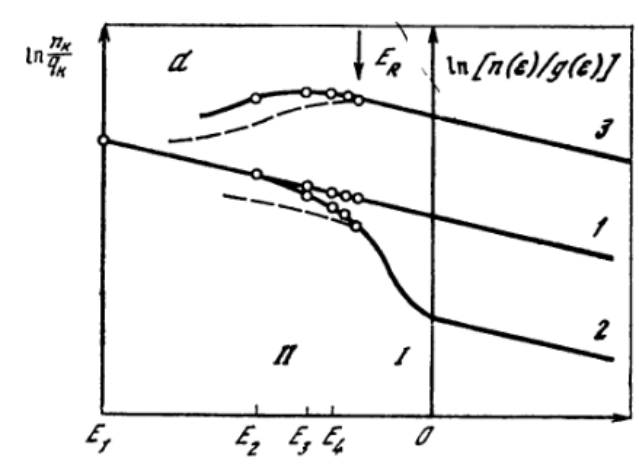
\includegraphics[width=0.5\linewidth]{excited_molecules.png}
	\end{center}
	\caption{Схема, поясняющая характерные распределения атомов по возбужденным состояниям~\cite{biberman}}
	\label{fig:excited_molecules}
\end{figure}

Излучение плазмы обедняет заселенность возбужденных состояний, замедляет ионизацию, ускоряет рекомбинацию. Характерно, что роль радиационных процессов резко уменьшается по мере приближения к границе непрерывного спектра~\cite{biberman}.

Населенности уровней определяются системой кинетических плазмохимических уравнений баланса, записанной для каждого из возбужденных состояний с учетом всевозможных элементарных процессов, обедняющих
или населяющих данный уровень.

Важнейшние процессы -- (1) возбуждение/тушение электронным ударом; (2) ионизация электронным ударом	и тройная рекомбинация; (3) возбуждение и тушение при столкновении с атомом в основном
состоянии; (4) ионизация в атом-атомных столкновениях и трехчастичная рекомбинация; (5) ассоциативная ионизация и диссоциативная рекомбинация; (6) спонтанные радиационные переходы между дискретными состояниями; (7) радиационная рекомбинация и фотоионизация~\cite{biberman}:

\begin{align*}
	(1)\;A_k + e &\leftrightarrow A_m + e;\\
	(2)\;A_k + e &\leftrightarrow A^{+} + 2e;\\
	(3)\;A_k + A_1 &\leftrightarrow A_m + A_1;\\
	(4)\;A_k + A_1 &\leftrightarrow A^{+} + e + A_1;\\
	(5)\;A_k + B &\leftrightarrow AB^{+} + e;\\
	(6)\;A_k &\rightarrow A_m + \hbar\omega;\;k>m\\
	(7)\;A_k + \hbar\omega &\rightarrow A^{+} + e;\;\hbar\omega\geq E_k\\
\end{align*}

Уравнение,
определяющее концентрацию возбужденных частиц в $k$-м состоянии:

\begin{equation*}
	\frac{dn_k}{dt} = \sum\limits_{m, q}(n_m\omega_{mk}^q-n_k\omega_{km}^q)+F_k-n_kG_k,
\end{equation*}

где $\omega_{km}^q$ -- вероятность перехода из $k$ в $m$ в процессе $q$. Суммирование проводится по всем дискретным состояниям. $F_k$ -- источник образования атомов в $k$-м состоянии за счет процессов, в которых не участвует рассматриваемый атом
или его ион (например, диссоциативная рекомбинация с образованием возбужденного атома в $k$-м состоянии). Группа процессов $G_k$ описывает гибель возбужденных атомов в результате процессов, в которых не образуются
атомы рассматриваемого элемента ни в основном, ни в возбужденных состояниях (ассоциативная ионизация). Уравнение для концентрации электронов записывается аналогично.

Важно: система уравнений записана в простом случае: не учтены потери частиц на стенках системы, где удерживается плазма (либо потери на периферии), не учтён вылет плазмы и прочие условия.

\section{Динамика заряженных частиц в электрическом и магнитном полях}
\label{sec.4}

\subsection{Движение в скрещенных электрическом и магнитном полях.}
\label{sec.4.1}
(Ландау том 2(задачи) Котельник лекции)

Движение заряда в постоянном электрическом/магнтном или обоих полях: Ландау том2, параграфы 21-22(вроже это совсем 
примитивно, в конце есть задачи, хз будут ли это спрашивать).

\subsection{Дрейфовое приближение, разновидности дрейфового приближения.}
\label{sec.4.2}
Когда $\rho_H\ll l$, a $2\pi/\omega_B \ll \tau$, где $l$ - характерный масштаб изменения полей, a $\tau$ - характерное
время изменения полей, движение частицы можно разделить на быстрое вращение и медленное движение центра окружности.
Такое медленное движение называют дрейфом. Далее рассмотрим основные типы дрейфового движения.

\subsubsection{Электрический дреф}
\label{sec.4.2.1}
Запишем уравнение движения(пока для нерелятивизма):

\begin{equation}
    \begin{cases}
    \label{eq.4.2.1-motion}
        dr/dt = \upsilon \\
        dp/dt = e E + e/c [\upsilon \times B]
    \end{cases}
\end{equation}
легко видеть, что если перейти в систему, которая движется со скоростью $\upsilon_E = c\frac{E\times B}{B^2}$, то
уравнения движения примут вид:

\begin{equation}
    \begin{cases}
    \label{eq.4.2.2-motion}
    \dot{v_x}'=  \frac{eB}{mc} v'_y \\
    \dot{v_y}'= -\frac{eB}{mc} v'_x \\
    \dot{v_z}'=  \frac{e}{m} E_{\parallel}
    \end{cases}
\end{equation}
первые два уравенения дают движение по окружности, а третье - есть движение вдоль магнитного поля. В итоге в сопутствующей
системе отсчета (та, что со штрихом) имеем спираль. $\upsilon_E$ называют электрическим дрейфом, т.к. он вызван 
электрическим полем. По сути это дрейф нулевого порядка, тут поля постоянные и никаких неоднородностей нет. В плазме,
как правило, эта скорость мала по сравнению с тепловой, по этому этот дрейф отосят к первому порядку.
Также можно записать выражение для радиус-вектора ведущего центра (воображаемого центра дрейфующей системы). Есть два
способа это сделать:

\begin{equation}
    \label{eq.4.2.3-R1}
        \mathbf{R}'=\mathbf{r} + \frac{\mathbf{v}' \times \mathbf{B}}{\omega_H}
\end{equation}

\begin{equation}
    \label{eq.4.2.3-R2}
        \mathbf{R}=\mathbf{r} + \frac{\mathbf{v} \times \mathbf{B}}{\omega_H}
\end{equation}
В случае ~\ref{eq.4.2.3-R1} частица в сопутствующей с.о. заметает цилиндр (радиус ларморовской окружности постоянный), а
в случае ~\ref{eq.4.2.3-R2} будет гофрированная поверхность.

В релятивистском случае есть более общая офрмула для $\upsilon_E$, получаемая из преобразований Лоренца:

\begin{equation}
    \label{eq.4.2.4}
    \upsilon_E=c \frac{1-\sqrt{1-4\xi^2}}{2\xi^2} \frac{E \times B}{B^2 + E^2}
\end{equation}

где $\xi = |E\times B / (B^2 + E^2)|$. Легко видель, что, как с случае $E<B$, так и в обратном, это выражение дает 
скорость меньше скорости света. (???? $E=B$ ???).

\subsubsection{Дрейф под действем малой силы}
\label{sec.4.2.2}
В общем случае выражение для дрейфа получается из электрического заменой $e\mathbf{E}$ на $\mathbf{F}$:

\begin{equation}
    \label{eq.4.2.5}
    \upsilon_F=\frac{c}{e} \frac{\mathbf{F} \times \mathbf{B}}{B^2}
\end{equation}
также её можно получить усредняя уравнение движения $m\frac{d\mathbf{v}}{dt}=\mathbf{F} + \frac{e}{c} \mathbf{v}\times\mathbf{B}$
по периоду циклотронного вращения. Строго говоря, в уравнении~\ref{eq.4.2.5} стоит усредненная поперечная сила 
$\langle F_{\parallel} \rangle$, вила вдоль магниного поля дает нулевой вклад в дрейф. В случае, когда сила $F$ мала, есть
простой способ вычисления скорости дрейфа - надо усреднить по траектории(окружности), при остутствии силы $F$.

\subsubsection{Гравитационный дрейф}
\label{sec.4.2.3}

Пусть в качестве малой силы выступает гравитационная сила $m\mathbf{g}$. Скорость такого дрейфа 
$\upsilon_g=\frac{mc}{e} \frac{\mathbf{g}\times\mathbf{B}}{B^2}$ зависит от заряда частицы. Это вызывает ток в направлении $\upsilon_g$.

\subsubsection{Градиентный дрейф}
\label{sec.4.2.4}

Пусть электрического поля нет, а у магнитного есть градиент, перпендикутярный самому полю. Выполняя усреднение по
невозмущенной орбите легко получть: $\upsilon_{\nabla B}=\frac{v_{\perp}^2}{2\omega_B} \frac{\mathbf{B}\times\nabla_{perp}B }{B^2}$.

\subsubsection{Центробежный дрейф}
\label{sec.4.2.5}
В отстутствии внешней силы частица может иметь некоторую проекцию скорости на направление магнитного поля:
$\upsilon=v_{\parallel}  \frac{\mathbf{B}}{B}$, обозначим $\mathbf{h}= \mathbf{B}/B$. Если линии магнитного поля имеют некоторый
имеют некоторый изгиб, то на частицу будет действовать центробежная сила: $\mathbf{F}=-m\frac{d\upsilon}{dt}$. Распишем
производную от скорости:

\begin{equation}
    \label{eq.4.2.5-u}
    \frac{d\upsilon}{dt}=\frac{\partial \upsilon}{\partial t} + (\upsilon \nabla) \upsilon,
\end{equation}
где второе слагаемое есть движеие ведущего центра - это и есть центробежный дрейф, и выражение для скорости дрейфа:

\begin{equation}
    \upsilon_{cf} = -\frac{\mathbf{h}}{\omega_B} \times (\upsilon \nabla) \upsilon
\end{equation}
выражение для скорости можно упростить, если подставить выражения для скорости ведущего центра в нулевом порядке
и учесть, что в плазме $E/B \ll v/c$. Тогда выражение примет вид:

\begin{equation}
    \upsilon_{cf} = \frac{v_{\parallel}^2}{\omega_B} \mathbf{h} \times (\mathbf{h}\nabla)\mathbf{h},
\end{equation}
эта скорость направлена по бинормали магнитной линни и зависит от знака заряда.

\subsubsection{Поляризационный дрейф}
\label{sec.4.2.6}

Первое слагаемое в выражении~\ref{eq.4.2.5-u} отвечает за поляризоционый дрейф.

\begin{equation}
    \upsilon_{pol} = \frac{\mathbf{h}}{\omega_B} \times \frac{\partial \upsilon}{\partial t},
\end{equation}
далее подставляя выражение для скорости ведущего центра и учитывая, что электрическое поле близко к потенциальному
можно получить:

\begin{equation}
    \upsilon_{pol} = \frac{c}{B\omega_B} \frac{\partial \mathbf{E}_{\perp}}{\partial t},
\end{equation}
она зависит от заряда, по этому в переменном поле плазма поляризуется. Поскольку плазма это проводник, постояную
поляризацию разделеными зарядами создать нельзя, но когда есть переменное электрическое поле, возникает переменный 
поляризационный ток и он вызывает реальную поляризацию плазмы.

\subsubsection{Дрейф в неоднородном электрическом поле}
\label{sec.4.2.7}
Аналогично магнитному полу, получаем для скорости дрейфа:

\begin{equation}
    \upsilon_{\nabla E} = \frac{c\rho_B^2}{4 B^2} \nabla^2_{\perp}\mathbf{E}\times \mathbf{B},
\end{equation}
она зависит от заряда, и создает ток, это т.н. эффект конечного ларморовского радиуса.

\subsection{Заряженная частица в высокочастотном поле}
\label{sec.4.3}
(тут только нерелятовистский случай)

Пусть есть в.ч. поле: $\mathbf{E}=Re\mathbf{E}(\mathbf{r}\exp(-i\omega t), \mathbf{B}=Re\mathbf{B}(\mathbf{r}\exp(-i\omega t)$, где $\mathbf{E}(\mathbf{r}), \mathbf{B}(\mathbf{r})$ медленно меняющиеся амплитуды (по сравнению с характерым
ларморовским радиусом). Тогда движенеи разбивается на медленный дрейф и быстрые осцилляции: $\mathbf{r}=\mathbf{R}+\mathbf{\rho}$. 
Тогда разложим электрическое поле(магнитное убираем, т.к. нерелятивизм): $E(\mathbf{r})=E(\mathbf{R})+(\mathbf{\rho} \nabla)E(\mathbf{R})$. В нулевом приближении мы принебрегаем вторым членом и уравнение движения в первом порядке имеет 
следующий вид(? $\mathbf{R}$ убираем т.к. меняется слабо?):

\begin{equation}
    \label{eq.4.3-0}
    \ddot{\mathbf{\rho}}=\mathbf{E}(\mathbf{R}) \frac{e}{m} \exp(-i\omega t).
\end{equation}
В следующем поярдке усредним по периоду $2\pi/\omega$ радиус вектор ($\rho$ уйдет, т.к. в среднем 0):

\begin{equation}
    \label{eq.4.3-1}
    \ddot{\mathbf{R}}=-\frac{-e^2}{m^2 \omega^2}\langle \mathbf{E} \exp(-i\omega t) \nabla \mathbf{E} \exp(-i\omega t) \rangle, 
\end{equation}
подставляя сюда выражение~\ref{eq.4.3-0}, получаем выражение для пондермоторного силы:

\begin{equation}
    \label{eq.4.3pf}
    \ddot{\mathbf{R}}=-\frac{-e^2}{4 m^2 \omega^2} \nabla |E|^2.
\end{equation}
(что еще тут ?)

\subsection{Понятие адиабатического инварианта}
\label{sec.4.4}

\subsubsection{Понятие адиабатического инварианта}
\label{sec.4.4.1}
Площадь потока матнитного поля $\Upphi=\pi \rho B$ через ларморовскую окружность в сопутствующей системе является
адиабатическим инвариантом - приближенно сохраняется при медленном изменении полей. Постоянство следует из закона
Фарадея: $\mathcal{E}=-\dot{\Upphi}/c$, где по законе Ома $\mathcal{E}=IR=0$, т.к. сопративления нет т.к. принебрегаем
столкновениями.

Для случая частицы движузейся в однородных электрическом и магнитных полях, в общем случае адиабат. инвариант есть:

\begin{equation}
    \label{eq.4.3pf}
    J_{\perp} = \frac{1}{2\pi} \oint \mathbf{P}_{\perp} d\mathbf{r}_{\perp},
\end{equation}
где интеграл берется по пероду вращения частицы в с.с.о. Далее используя теорему Стокса можно получить, что:

\begin{equation}
    \label{eq.4.3pf}
    J_{\perp} = \frac{m\upsilon_{\perp}^2}{2\omega_B}=\frac{|e|}{2\pi c} \Upphi, 
\end{equation}
В общем случае адиабат. нвариантам являются следующие величины: $\Upphi$, $\gamma \mu$, $p_{\perp}^2/B$.

\subsubsection{Продольный адиабатический инвариант}
\label{sec.4.4.2}
В магнитных пробках, в нулевом приближении частица движется вдоль силовой линии от поворота к повороту. Интеграл вдоль
такого движения есть т.н. продольный адиабат. инвариант:

\begin{equation}
    \label{eq.4.3pf}
    J_{\parallel} = \frac{1}{2\pi}\oint\mathbf{P}_{\parallel}ds=1/\pi \int \sqrt{2m \left(\varepsilon - e\phi - \mu B - 0.5m\upsilon_E^2 \right)}. 
\end{equation}
Этот интеграл зависит от следующих параметров $J_{\parallel}=J_{\parallel}(x_0, y_0, \varepsilon, \mu)$, где $x_0, y_0$
есть координаты пересечения силовой линии с поверхностью рассекающую магнитную ловушку поперек.

\subsubsection{Третий адиабатический инвариант}
\label{sec.4.4.3}

В магнитной ловушке частица движется от одного конца к другому, смещаясь вдоль экватора, заметая некую поверхность - 
дрейфовую оболочку. Если магнитное поле и потенциал медленно меняются, сохраняется магнитный поток через сечение 
дрейфовой оболочки:

\begin{equation}
    \label{eq.4.3pf}
     \Upphi_{dr}= \int_{S_{dr}} \mathbf{B}d\mathbf{S}.
\end{equation}

Эти адиабат. инварианты удобны для нахождения завичимости энергии частицы от времени.

\section{Магнитная гидродинамика плазмы}

\subsection{Уравнения движения плазмы в магнитном поле, проникновение магнитного поля в плазму, вмороженность магнитного поля}

Здесь и ниже будем рассматривать только простую плазму - состоящую из электронов и ионов одного сорта. Запишем уравнения гидродинамики. Их вывод смотри в Доп. 1:
\begin{align}
	&\pdv{N_\alpha}{t}+\div{ \left( N_\alpha \vb{v}_\alpha \right) } = 0 ,\\
	&m_\alpha N_\alpha \left( \pdv{\vb{v}_\alpha}{t} +(\vb{v}_\alpha \cdot\grad )\vb{v}_\alpha \right) = -\grad{P_\alpha} + e_\alpha N_\alpha\vb{E} + \frac{e_\alpha N_\alpha}{c}[\vb{v}_\alpha \times \vb{B}] + \vb{F}_{fric,\alpha},
\end{align}
где $\alpha = e, i$, $\vb{F}_{fric,\alpha}$~---~эффективная сила трения на сорт частиц $\alpha$ со стороны другого сорта.
Это уравнения \textit{двухжидкостной гидродинамики}.
Можно ввести макроскопические плотность тока и заряда:
\begin{align*}
	&\rho_e = \sum_\alpha e_\alpha N_\alpha = e N_i - e N_e, \\
	&\vb{j} = \sum_\alpha e_\alpha N_\alpha \vb{v}_\alpha = e N_i \vb{v}_i - e N_e \vb{v}_e
\end{align*}
и замкнуть уравнения гидродинамики с уравнениями Максвелла:
\begin{align}
	\curl\vb{E} = -\frac{1}{c}\pdv{\vb{B}}{t}, \\
	\curl\vb{B} = \frac{4\pi}{c}\vb{j}, \\
	\divergence{\vb{B}} = 0,\\
	\rho_e = 0
\end{align}
Где мы выкинули ток смещения $\partial\vb{E}/\partial t$, т.к. мы будем рассматривать процессы со скоростями сильно медленнее скорости света, а последнее равенство говорит, что мы рассматриваем квазинейтральную (незаряженную) плазму.

В таком виде уравнения решать сложно. Заметим, что массу в основном переносят ионы. Запишем уравнения для элемента массы плазмы $\rho = m_e N_e + m_i N_i$, движущейся со скоростью $\vb{V} = (m_e N_e \vb{v}_e + m_i N_i \vb{v}_i)/\rho$
\begin{align}
	\pdv{\rho}{t} + \divergence{\left( \rho \vb{V} \right)} = 0 \\
	\rho\left( \pdv{\vb{V}}{t} + (\vb{V}\cdot\grad)\vb{V} \right) = -\grad{(P_e + P_i)} + \frac{1}{c}[\vb{j}\times\vb{B}]
\end{align}
Слагаемые с силой трения вычитаются по третьему закону Ньютона.
По сути эти уравнения - гидродинамические уравнения, описывающие проводящую жидкость. Так как здесь явно нет ионов и электронов - это уравнения \textit{одножидкостной} гидродинамики.
Обычно $\vb{j}$ в уравнении Эйлера выражают из уравнений Максвелла: $\vb{j} = c/4\pi\curl\vb{B}$.

Для окончательного замыкания уравнений гидродинамики и уравнений Максвелла нам нужен закон Ома, т.е. зависимость между векторами $\vb{j}$ и $\vb{E}$. 

\vspace{5mm}
\textbf{1. Вывод Токмана:} 

Вернёмся к уравнению Эйлера для электронов. Так как с помощью гидродинамики мы описываем процессы на масштабах существенно более медленные, чем, например, столкновения, то запишем уравнение Эйлера в пределе $\omega \ll \nu$, где $\omega$~---~характерная частота процесса, $\nu$~---~частота столкновений (электрон-ионных). В таком случае слагаемое $m_e N_e \dd \vb{v}_e/\dd t$ в левой части много меньше, чем сила трения в правой части, которую можно записать в виде $\nu m_e N_e (\vb{v}_e - \vb{v}_i) = -\nu m_e \vb{j} / e$. Итого имеем:
\begin{equation}
	\label{eq.5.euler}
	0 \approx -\grad{P_e} - e N_e \vb{E} - \frac{e}{c}[\vb{v}_e \times \vb{B}] + \frac{\nu m_e}{e}\vb{j}
\end{equation}
Заметим, что $\vb{j} = e (N_i \vb{v}_i - N_e \vb{v}_e) \approx e N (\vb{v}_i - \vb{v}_e) \approx e N \vb{V} $, где во втором равенстве использовалось условие квазинейтральности $N_e \approx N_i = N$, а в третьем - малость массы электронов $\vb{V} \approx \vb{v}_i$. Из этого соотношения выражаем $\vb{v_e}$:
\begin{equation}
	\vb{v}_e = \vb{v}_i - \frac{\vb{j}}{eN} = \vb{V} - \frac{\vb{j}}{eN}
\end{equation}
Тогда переписываем уравнение~\eqref{eq.5.euler} в следующем виде:
\begin{equation}
	\label{eq.5.Ohm}
	\vb{j} = \sigma \left( \vb{E} + \frac{1}{c}[\vb{V}\times\vb{B}] - \frac{1}{ceN}[\vb{j}\times\vb{B}] + \frac{\grad{P_e}}{eN} \right)
\end{equation}
где $\sigma = e^2 N_e / m \nu$.

Рассмотрим теперь уравнение одножидкостной гидродинамики в том же приближении $\omega \ll \nu$, т.е. по сути будем искать состояние равновесия. Получим:
\begin{equation}
	0 \approx -\grad{\left( P_e + P_i \right)} + \frac{1}{c}[\vb{j}\times\vb{B}]
\end{equation}
Подставляя это в уравнение~\eqref{eq.5.Ohm} получаем окончательный вид закона Ома:
\begin{equation}
	\vb{j} = \sigma \left( \vb{E} + \frac{1}{c}[\vb{V}\times\vb{B}] - \frac{\grad{P_i}}{eN} \right)
\end{equation}

Оценим по порядку величины второе и третье слагаемые.
Второе:
\begin{align*}
	\curl\vb{E} = -\frac{1}{c}\dv{\vb{B}}{t} \\
	B \sim \frac{c\tau}{L} E = \frac{c}{V} E
\end{align*}
Следовательно втрой член одного порядка с первым

Третье слагаемое:
\begin{align*}
	\frac{\grad P_i}{N e} \sim \frac{N T}{N e L} = \frac{T}{eL} \\
	V \text{vs.} \frac{cT}{BeL} \sim v_{d}
\end{align*}
где $v_{d}$~---~скорость дрейфа в неоднородном поле (см.~\ref{sec.4.2.4}). Этим слагаемым можно пренебречь, когда дрейфовая скорость много меньше средней скорости ионов. Обычно работаем именно в таком приближении.

\vspace{5mm}
\textbf{2. Вывод Котельникова:} 

Просто предположим линейную зависимость между током $\vb{j}$ и электрическим полем в системе отсчёта, движущейся с элементом плазмы $\vb{E}'$. Преобразование Лоренца в лабораторную систему при малых скоростях $V \ll c$ имеет вид:
\begin{equation}
	\vb{E}' = \vb{E} + \frac{1}{c}[\vb{V}\times \vb{B}]
\end{equation}
тогда закон Ома имеет вид:
\begin{equation}
	\vb{j} = \Sigma\left( \vb{E} + \frac{1}{c}[\vb{V}\times \vb{B}] \right)
\end{equation}

\textbf{Итоговая система одножидкостной МГД:}
\begin{align}
	\label{eq.5.mgd1}
	&\pdv{NM}{t} + \divergence{\left( NM\vb{V} \right)} = 0 \\
	\label{eq.5.mgd2}
	&N M \dv{\vb{V}}{t} = -\grad{P} + \frac{1}{4\pi}\left[\left[ \curl{\vb{B}} \right]\times\vb{B}\right] \\
	\label{eq.5.mgd3}
	&\curl{\vb{B}} = \frac{4\pi}{c}\vb{j} \\
	\label{eq.5.mgd4}
	&\curl{\vb{E}} = -\frac{1}{c}\pdv{\vb{B}}{t} \\
	\label{eq.5.mgd5}
	&\divergence{\vb{B}} = 0 \\
	\label{eq.5.mgd6}
	&\vb{j} = \sigma\left( \vb{E} + \frac{1}{c}[\vb{V}\times\vb{B}] \right)
\end{align}

Возьмём ротор от уравнения~\eqref{eq.5.mgd3}:
\begin{align*}
	&\curl{[\curl{\vb{B}}]} = \frac{4\pi\sigma}{c}\curl{\left( \vb{E} + \frac{1}{c}[\vb{V}\times\vb{B}] \right)} \\
	&-\Delta\vb{B} = \frac{4\pi\sigma}{c^2}\left( -\pdv{\vb{B}}{t} + \curl{[\vb{V}\times\vb{B}]} \right) \\
	&\pdv{\vb{B}}{t} = \curl{[\vb{V}\times\vb{B}]} + \frac{c^2}{4\pi\sigma}\Delta\vb{B}
\end{align*}
Оценим слагаемые в правой части:
\begin{align*}
	&\curl{[\vb{V}\times\vb{B}]} \sim \frac{VB}{L} \\
	&\frac{c^2}{4\pi\sigma}\Delta\vb{B} \sim \frac{c^2B}{4\pi\sigma L^2}
\end{align*}
Вводят \textit{магнитное число Рейндольдса} $R_m$ - отношение этих членов:
\begin{equation*}
	R_m = \frac{4\pi\sigma VL}{c^2}
\end{equation*}
В зависимости  от величины $R_m$ реализуются различные ситуации:

\vspace{5mm}
\textbf{1. $R_m \ll 1$ (маленькая проводимость/большой размер плазмы/быстрые потоки):}

В таком случае не учитываем слагаемое $\vb{V}\times\vb{B}$ и получаем уравнение:
\begin{equation}
	\pdv{\vb{B}}{t} = \frac{c^2}{4\pi\sigma}\Delta\vb{B} \equiv D_m\Delta\vb{B}
\end{equation}
Это уравнение диффузии, которое описывает скинирование магнитного поля в плазме.
Глубина проникновения переменного магнитного поля в плазму оценивается как $\sqrt{2D_m\tau}$, где $\tau$~---~характерное время колебаний магнитного поля $\tau\sim 1/\omega$, т.е.
\begin{equation*}
	\delta = \frac{c}{2\pi\sigma\omega}
\end{equation*}
Это выражение для толщины скин-слоя. Отметим, что точно такое же выражение получается при рассмотрении проникновения переменного тока в проводник с конечной проводимостью.

\vspace{5mm}
\textbf{2. $R_m \gg 1$ (большая проводимость):}

Этот предел соответствует \textit{идеальной магнитной гидродинамике}.
Уравнения в таком случае принимают вид:
\begin{align}
	\label{eq.5.imgd1}
	&\pdv{N}{t} + \divergence{\left( N\vb{V} \right)} = 0 \\
	\label{eq.5.imgd2}
	&N M \dv{\vb{V}}{t} = -\grad{P} + \frac{1}{4\pi}\left[\left[ \curl{\vb{B}} \right]\times\vb{B}\right] \\
	\label{eq.5.imgd3}
	&\pdv{\vb{B}}{t} = \curl{[\vb{V}\times\vb{B}]}
\end{align}

\vspace{5mm}
\textbf{Вмороженность магнитного поля:}

Качественно~---~силовые линии магнитного поля как бы приклеены к частицам плазмы, т.е. оно никогда не пересекает траектории частиц.  Силовые линии магнитного поля перемещаются по траекториям частиц.

\begin{figure}[h!]
    \center{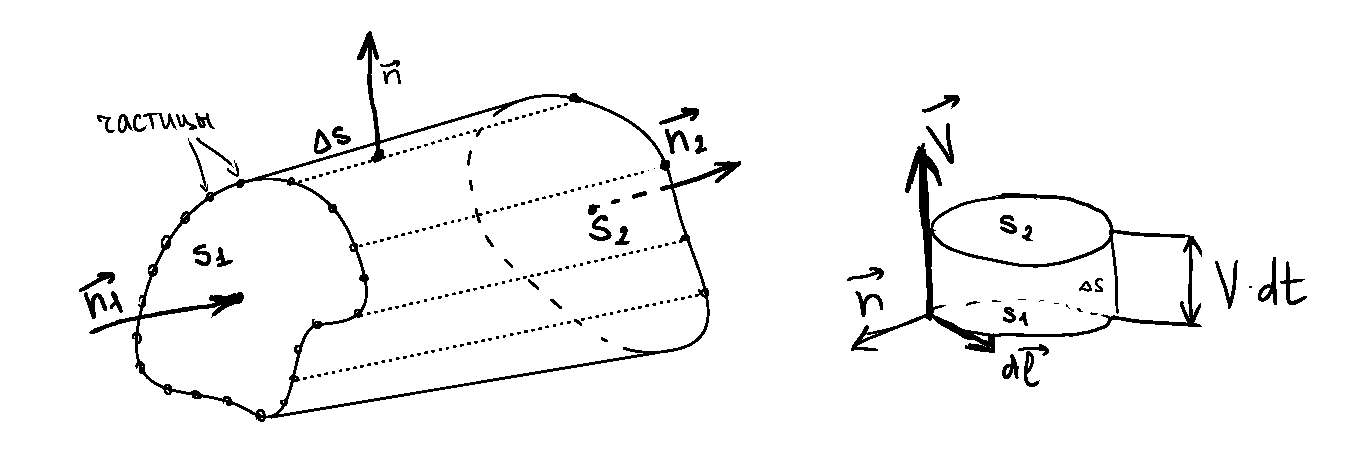
\includegraphics[width=1\linewidth]{5.flow.pdf}}
    \caption{\label{fig.5.flow} Геометрия при выводе вмороженности.}
\end{figure}

\uline{Доказательство:}
Рассчитаем изменение потока магнитного поля за интервал времени $\dd t$ через поверхность <<трубки>>, образованной траекториями частиц плазмы (см. Рис.~\ref{fig.5.flow}). Изменение этого потока связано с двумя эффектами: изменением амплитуды магнитного поля и изменением площади поверхности трубки. В приближении бесконечно малых $\dd t$ эти эффекты учитываем независимо, т.е.:
\begin{equation}
	\label{eq.5.frozen}
	\Phi_2 - \Phi_1 = \iint\limits_S (\vb{B}_2 - \vb{B}_1)\dd \vb{S} + \iint\limits_{S_2 - S_1}\vb{B}_1\dd\vb{S}
\end{equation}
Так как магнитное поле бездивергентно, то его поток через любую замкнутую поверхность равен нулю, т.е.
\begin{equation*}
	\iint\limits_{S_2}\vb{B}_1\dd\vb{S} + \iint\limits_{\Delta S}\vb{B}_1\dd\vb{S} - \iint\limits_{S_1}\vb{B}_1\dd\vb{S} = 0
\end{equation*}
где знак "$-$" перед слагаемым $S_1$ связан с направлением нормали, которую мы выбрали (см. Рис.~\ref{fig.5.flow}). Из этого равенства следует, что в выражении~\eqref{eq.5.frozen} первый множитель можно вычислить следующим образом:
\begin{equation}
	\label{eq.5.flow1}
	\iint\limits_{S_2 - S_1}\vb{B}_1\dd\vb{S} = -\iint\limits_{\Delta S} \vb{B}_1\dd\vb{S} = -\oint\limits_{l_1} \left( \vb{n}\vb{B}_1 \right) \dd l\,V\,\dd t
\end{equation}
где $V\dd t$~---~<<ширина>> ленточной поверхности $\Delta S$, $\vb{n}$~---~нормаль к ней. Эту нормаль можно записать в следующем виде:
\begin{equation*}
	\vb{n} = \frac{[\dd\vb{l}\times\vb{V}]}{\dd l\, V}
\end{equation*}
Тогда выражение~\eqref{eq.5.flow1} записывается в следующем виде:
\begin{equation*}
	\iint\limits_{S_2 - S_1}\vb{B}_1\dd\vb{S} = -\dd t \oint\limits_{l_1} [\dd\vb{l}\times\vb{V}]\vb{B}_1 = -\dd t \oint\limits_{l_1} [\vb{V}\times\vb{B}_1]\dd\vb{l} = -\dd t\iint\limits_{S_1}\curl[\vb{V}\times\vb{B}_1]
\end{equation*}
где в предпоследнем равенстве мы сделали циклическую перестановку в смешанном произведении, а в последнем применили теорему Стокса.

В итоге переписываем уравнение~\eqref{eq.5.frozen}:
\begin{equation*}
	\frac{\Phi_2 - \Phi_1}{\dd t} = \iint\limits_{S_1}\left( \frac{\vb{B}_2 - \vb{B}_1}{\dd t} - \curl[\vb{V}\times\vb{B}_1] \right)\dd\vb{S} \stackrel{\dd t\rightarrow 0}{=} \iint\limits_{S_1}\left( \pdv{\vb{B}}{t} - \curl[\vb{V}\times\vb{B}] \right)\dd\vb{S} = 0
\end{equation*}
где последнее равенство верно в силу уравнений идеальной МГД~\eqref{eq.5.imgd3}.
Таким образом получаем, что поток через любую трубку, образованную траекториями плазмы является константой. Так как можем взять сколь угодно тонкую трубку, то получается, что силовые линии как бы приклеены к частицам плазмы и силовые линии магнитного поля совпадают с траекториями частиц.

Ещё следствия из вмороженности:
\begin{itemize}
	\item Частицы, находящиеся на одной магнитной линии, всегда будут находиться на одной магнитной линии.
	\item Сохраняется топология магнитного поля, т.е. не допускается появление разрывов в магнитных линиях, например, как в магнитной рекомбинации. Разрешены только топологически непрерывные изменения линий магнитного поля.
	\item Плазма не может расширяться поперёк магнитного поля.
\end{itemize}

Очевидно, что в реальности из-за конечной проводимости все эти эффекты верны только приближённо. Например, магнитное поле может диффундировать в плазму. С другой стороны это можно трактовать как смещение плазмы поперёк магнитного поля.

\subsection{Законы сохранения в идеальной одножидкостной МГД}

В целом уравнения гидродинамики выглядят как уравнения сохранения:
\begin{equation}
	\label{eq.5.conserve}
	\pdv{N}{t} + \div{\vb{J}} = 0
\end{equation}
где $N$~---~плотность некой величины, а $\vb{J}$~---~её поток.
Явно перепишем уравнения МГД~\eqref{eq.5.imgd1}--\eqref{eq.5.imgd3} в форме законов сохранения~\eqref{eq.5.conserve}. Первое уравнение уже записано в таком виде:
\begin{align}
	\label{eq.5.cons1}
	&\pdv{N}{t} + \divergence{\left( N\vb{V} \right)} = 0 \\
	\label{eq.5.cons_fin1}
	&\dv{\rho}{t} = 0
\end{align}
По сути это уравнение~---~\textit{закон сохранения массы} $\rho = NM$.

\vspace{5mm}
Преобразуем уравнение Эйлера:
\begin{equation*}
	\label{eq.5.cons2}
	N M \left( \pdv{\vb{V}}{t} + \left( \vb{V}\cdot\grad \right)\vb{V} \right) = -\grad{P} + \frac{1}{4\pi}\left[\left[ \curl{\vb{B}} \right]\times\vb{B}\right]
\end{equation*}
Распишем последнее слагаемое:
\begin{equation*}
	\left[\left[ \curl{\vb{B}} \right]\times\vb{B}\right] = -\left[\vb{B}\times\left[ \curl{\vb{B}} \right]\right] = -\frac{1}{2}\grad{B^2} + \left( \vb{B} \cdot\grad \right)\vb{B}
\end{equation*}
Это выражение можно записать в тензорном виде:
\begin{equation*}
	\begin{split}
		\left( -\frac{1}{2}\grad{B^2} + \left( \vb{B} \cdot\grad \right)\vb{B} \right)_\nu = -\frac{1}{2}\pdv{B^2}{x_\nu} + B_\mu\pdv{B_\nu}{x_\mu}= -\frac{1}{2}\pdv{}{x_\mu}\left( B^2 \delta_{\mu\nu} \right) + \pdv{}{x_\mu}\left( B_\mu B_\nu \right) - B_\nu\pdv{B_\mu}{x_\mu} =\\= \pdv{}{x_\mu}\left( -\frac{B^2}{2} \delta_{\mu\nu} + B_\mu B_\nu \right)
	\end{split}
\end{equation*}
где было использовано $\partial B_\mu/\partial x_\mu = 0$ ($\div{\vb{B}}=0$).

Умножим уравнение~\eqref{eq.5.cons1} на $M\vb{V}$ и сложим с уравнением~\eqref{eq.5.cons1}. Рассмотрим отдельно слагаемые с дивергенцией:
\begin{equation*}
	V_\nu \pdv{}{x_\mu}\left( NV_\mu \right) + NV_\mu\pdv{V_\nu}{x_\mu} = \pdv{}{x_\mu}\left( NV_\mu V_\nu \right)
\end{equation*}
В итоге уравнение Эйлера переписывается в следующем виде:
\begin{equation*}
	\pdv{}{t}\left( NM\vb{V} \right) + \div{\left( NM\overleftrightarrow{\vb{VV}} + \left( P + \frac{B^2}{8\pi} \right)\overleftrightarrow{\vb{I}} - \frac{1}{4\pi}\overleftrightarrow{\vb{BB}} \right)} = 0
\end{equation*}
\begin{equation}
	\pdv{}{t}\left( NM\vb{V} \right) + \div{\left( NM\overleftrightarrow{\vb{VV}} + P\overleftrightarrow{\vb{I}} + \overleftrightarrow{\vb{T}} \right)} = 0
\end{equation}
\begin{equation}
	\label{eq.5.momentum}
	\dv{\vb{\Pi}}{t} = - \div{\left( P\overleftrightarrow{\vb{I}} + \overleftrightarrow{\vb{T}} \right)}
\end{equation}
где $\overleftrightarrow{\vb{I}}$~---~единичный тензор $\delta_{\mu\nu}$, $\overleftrightarrow{\vb{BB}}$~---~обозначение тензора с компонентами $B_\mu B_\nu$.
Таким образом получили аналог \textit{закона сохранения импульса}: $\vb{\Pi}=NM\vb{V}$~---~это плотность импульса, а тензор $\overleftrightarrow{\vb{T}}$ называют \textit{тензором напряжений магнитного поля}. 	
Из уравнения~\eqref{eq.5.momentum} видно, что правая часть этого уравнения имеем смысл плотности силы $\vb{f}$, а полная сила получается интегрированием по объёму $\dd V$, который по теореме Гаусса преобразуется к интегралу по площади, ограничивающей $\dd V$. Таким образом тензоры $P\overleftrightarrow{\vb{I}}$ и $\overleftrightarrow{\vb{T}}$ определяют общую силу, действующую на маленькую площадку $\dd\vb{S}$.
Силу со стороны магнитного поля можно разделить на силу вдоль и поперёк магнитного поля:
\begin{equation*}
	T_{\mu\nu} = \frac{B_\mu B_\nu}{4\pi}-\frac{B^2}{8\pi}\delta_{\mu\nu} = p_m \left( \delta_{\mu\nu} - b_\mu b_\nu \right) - p_m b_\mu b_\nu = p_m (b_\perp - b_\parallel)
\end{equation*}
где $p_m = B^2 / 8 \pi$~---~<<магнитное>> давление. Таким образом, магнитное поле <<тянет>> площадку $\dd \vb{S}$ вдоль своего направления $\vb{B}/B$ и <<давит>> на площадку поперёк своего направления.

\vspace{5mm}
Рассмотрим третье уравнение идеальной МГД:
\begin{equation*}
	\label{eq.5.cons3}
	\pdv{\vb{B}}{t} = \curl{[\vb{V}\times\vb{B}]}
\end{equation*}
Преобразуем правую часть (ротор от векторного произведения раскрывается с использованием правила стрелок):
\begin{equation*}
	\curl{[\vb{V}\times\vb{B}]} = (\vb{B}\cdot\grad)\vb{V} - (\vb{V}\cdot\grad)\vb{B} - \vb{B}\,\text{div}{\vb{V}} + \vb{V}\,\text{div}{\vb{B}}
\end{equation*}
Распишем по компонентам:
\begin{equation*}
	\curl{[\vb{V}\times\vb{B}]}_\nu = B_\mu \pdv{V_\nu}{x_\mu} - V_\mu \pdv{B_\nu}{x_\mu} - B_\nu\pdv{V_\mu}{x_\mu} + V_\nu\pdv{B_\mu}{x_\mu} = \pdv{}{x_\mu}\left( B_\mu V_\nu - B_\nu V_\mu \right)
\end{equation*}
В итоге вмороженность магнитного поля тоже можно записать в виде некого закона сохранения:
\begin{equation*}
	\pdv{\vb{B}}{t} + \div{\left( \overleftrightarrow{\vb{VB}} - \overleftrightarrow{\vb{BV}} \right)} = 0
\end{equation*}

\vspace{5mm}
Вообще говоря уравнения гидродинамики обычно обрывают на уравнении переноса тепла, которое мы обычно не используем, т.к. оно не важно для рассмотрения волн, неустойчивостей и т.п. Его очевидно тоже можно записать в виде \textit{закона сохранения энергии}:
\begin{equation}
	\label{eq.5.cons_fin4}
	\pdv{Q}{t} + \div{\vb{q}} = 0
\end{equation}
где $Q$~---~плотность тепловой энергии $MN\langle \vb{V}\vb{V} \rangle - MN\langle V\rangle^2$. Вектор потока тепла $\vb{q}$ в запоминающемся виде не записывается, поэтому я его не пишу.

Если функции распределения локально максвелловские и поля слабые (т.е. нет, например, омического нагрева), то это уравнение переходит в уравнение теплопроводности:
\begin{equation}
	\label{eq.5.temp}
	\pdv{T}{t} = \div{\left( \chi \grad T \right)}
\end{equation}
где $\chi$~---~коэффициент температуропроводности. Он связан с коэффициентом теплопроводности $\varkappa = 3\chi/2N$.

Однако важно понимать, что вообще говоря, наличие внешнего магнитного поля делает плазму анизотропной, и эта анизотропия проявляется даже в переносе тепла.
Кинетическая теория (см.~\ref{sec.3}) даёт следующее выражение для коэффициента температуропроводности:
\begin{equation*}
	\chi_\alpha \sim  \frac{T_\alpha \tau_\alpha}{m_\alpha}
\end{equation*}
Введём длину свободного пробега $\lambda_\alpha = v_{T_\alpha} / \tau_\alpha$:
\begin{equation*}
	\chi_\alpha \sim \frac{\lambda_\alpha^2}{\tau_\alpha}
\end{equation*}
Выражение в таком виде совместно с уравнением~\eqref{eq.5.temp} несёт ясный физический смысл: характерный масштаб теплопроводности в пространстве равен $\lambda_\alpha$ и во времени $\tau_\alpha$. При этом наличие магнитного поля не влияет на движение вдоль магнитного поля, значит эти масштабы должны оставаться такими же.
В движении поперёк магнитного поля появляется ещё один характерный масштаб - Ларморовский радиус. Поэтому в сильном магнитном поле, т.е. если $\rho_\alpha \sim v_{T_\alpha} / \Omega_\alpha \ll \lambda_\alpha$, можно считать, что коэффициент поперечной теплопроводности записывается в следующем виде:
\begin{equation*}
	\varkappa_{\perp\alpha} \sim \frac{N_\alpha \rho_\alpha^2}{\tau_\alpha}
\end{equation*}

\begin{figure}[h!]
    \center{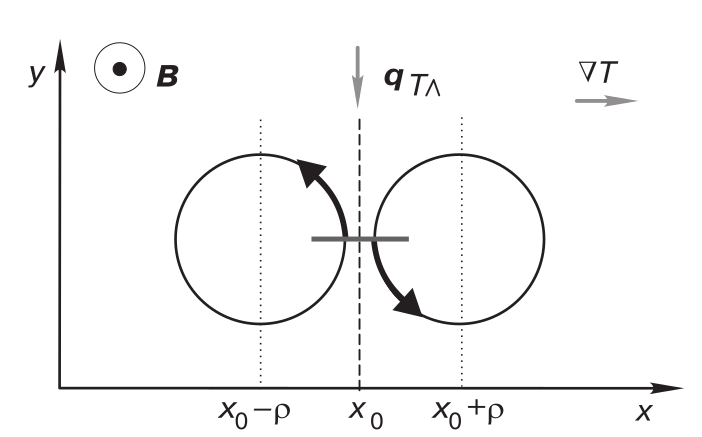
\includegraphics[width=0.5\linewidth]{5.slanted.png}}
    \caption{\label{fig.5.slanted} Возникновение <<косого>> потока тепла.}
\end{figure}

Строго говоря в замагниченной плазме есть ещё так называемый <<косой>> поток тепла. Его появление связано с тем, что при наличии градиента температур поток энергии через площадку, натянутую на вектора $\vb{B}$ и $\grad T$, оказывается отличен от нуля из-за того, что поток в одну сторону этой площадки создаётся более горячими электронами, а поток в другую - более холодными (см. Рис.~\ref{fig.5.slanted}).
Легко оценить нескомпенсированный потока тепла в такой ситуации: $q_x \sim N_e v_{T_e} \rho_e (\partial T_e/\partial x)$. Тогда в уравнении теплопроводности должно быть ещё следующее слагаемое:
\begin{equation*}
	\pdv{Q_e}{t} = \dots + \pdv{}{x}\left( N_e v_{T_e} \rho_e \pdv{T_e}{x} \right) = \dots + \pdv{}{x}\left(  \frac{N_e v_{T_e}^2}{\Omega_e}\pdv{T_e}{x} \right)
\end{equation*}
Таким образом в замагниченной плазме есть три разных коэффициента теплопроводности (продольной, поперечной, косой):
\begin{align*}
	&\varkappa_{\parallel\alpha} \sim \frac{N_\alpha \lambda_\alpha^2}{\tau_\alpha} \\
	&\varkappa_{\perp\alpha} \sim \frac{N_\alpha \rho_\alpha^2}{\tau_\alpha} \\
	&\varkappa_{\wedge\alpha} \sim \frac{N_\alpha v_{T_\alpha}^2}{\Omega_\alpha}
\end{align*}

\subsection{Двухжидкостное приближение}

Смотри начало.

\section{Неустойчивость плазмы}

\subsection{Равновесные конфигурации плазмы в магнитной гидродинамике, пинч}

Для рассмотрения неустойчивостей в плазме сначала надо определить равновесные конфигурации. Будем искать их в приближении идеальной МГД. Конфигурация плазмы является равновесной, если на плазму не действует сила. В таком случае уравнения, описывающую равновесную конфигурацию имеют вид:
\begin{align*}
	&\grad{P} = \frac{1}{c}[\vb{j}\times\vb{B}] \\
	&\curl\vb{B} = \frac{4\pi}{c}\vb{j} \\
	&\div{\vb{B}} = 0 \\
	&\div{\vb{j}} = 0
\end{align*}
Из первого уравнения следует, что $\vb{B}\cdot\grad{P} = \vb{j}\cdot\grad{P} = 0$. Это в свою очередь обозначает, что давление постоянно вдоль линий магнитного поля и линий тока (не путать направление тока $\vb{j}$ и направление потока массы $\vb{V}$ !). Значит плазма может расширяться только вдоль направлений $\vb{j}$ и $\vb{B}$. С другой стороны эти условия значат, что силовые линии $\vb{j}$ и $\vb{B}$ лежат на изобарах~---~поверхностях постоянного давления. По сути уже из этого следует, что единственный способ удержания плазмы и изоляции её от стенок камеры~---~это конфигурация, в которой поверхность камеры является поверхностью нулевого давления, а поверхности большего давления вложены в неё. Такой конфигурации соответствует тор. Однако для упрощения математики будем считать, что внешний радиус тора много больше внутреннего и будем считать, что локально мы имеем дело с цилиндром.

Перепишем в очередной раз слагаемое $\vb{B}\times[\curl{\vb{B}}]$:
\begin{equation*}
	\vb{B}\times[\curl{\vb{B}}] = \frac{1}{2}\grad{B^2} - \left( \vb{B}\cdot\grad \right)\vb{B}
\end{equation*}
Выделим в $\vb{B}$ модуль и направление: $\vb{B} = B\vb{h}$. После несложных преобразований получим:
\begin{equation*}
	\vb{B}\times[\curl{\vb{B}}] = \frac{1}{2}\grad_\perp B^2 - B^2\left( \vb{h}\cdot\grad \right)\vb{h}
\end{equation*}
где $\grad_\perp = \grad - \left( \vb{h}\cdot\grad \right)$~---~поперечный градиент. Производная поля ортов по направлению самого себя связано с кривизной линий поля $R$:
\begin{equation*}
	\left( \vb{h}\cdot\grad \right)\vb{h} = \frac{\vb{n}}{R}
\end{equation*}
где $\vb{n}$~---~нормаль к изогнутой силовой линии.
В итоге плотность силы можно записать в следующем виде:
\begin{equation*}
	\vb{f} = -\grad_\perp\left( P + \frac{B^2}{8\pi} \right) + \frac{B^2}{4\pi R}\vb{n}
\end{equation*}
Последнее слагаемое~---~это возвращающая сила связанная с кривизной магнитных линий; похоже на возвращающую силу в струне.

Рассмотрим сначала аксиально симметричные конфигурации~---~это так называемые \textit{пинчи}. В таком случае ток и магнитное поле могут зависеть только от радиальной координаты $r$. Тогда уравнение равновесия записывается в следующем виде:
\begin{equation*}
	\dv{p}{r} = -\dv{}{r}\frac{B_z^2}{8\pi} - \frac{1}{r^2}\dv{}{r}\frac{r^2 B_\theta^2}{8\pi}
\end{equation*}
Вообще это уравнение разрешает существование бесконечного числа конфигураций, но можно ограничиться только двумя предельными случаями.

\vspace{5mm}
\textbf{$\theta$-пинч}

Тета-пинч~---~это конфигурация, в которой отсутствует продольный ток и соответственно азимутальное магнитное поле. Такую конфигурацию можно создать, пустив азимутальный ток снаружи плазменного столба (по сути поместив плазму внутри соленоида). Тогда продольное магнитное поле будет удерживать плазму. Уравнение равновесия в этом случае выглядит следующим образом (силовые линии поля прямые, поэтому формально $R\rightarrow\infty$):
\begin{align*}
	&\dv{}{r}\left( p + \frac{B_z^2}{8\pi} \right) = 0 \\
	&p + \frac{B_z^2}{8\pi} = \text{const} = \frac{B_{vac}^2}{8\pi}
\end{align*}
где $B_{vac}$~---~магнитное поле вне плазмы. Эта простая конфигурация показывает, что плазма может вести себя как диамагнетик, т.е. уменьшать магнитное поле. При этом при $p = B_{vac}^2/8\pi$ магнитного поля внутри плазмы нет вообще. В таком случае на границе плазмы есть скачок магнитного поля и следовательно азимутальный ток, который и удерживает плазму (за счёт силы Ампера). Если давление плазмы превышает вакуумное давление магнитного поля, то равновесного состояния не существует и плазма не удерживается.

\vspace{5mm}
\textbf{$Z$-пинч}

В $z$-пинче ток течёт вдоль плазменного столба и конфигурация просто совпадает с проводом с током и азимутальным магнитным полем. Условие равновесия выглядит так (в данном случае $R=r$ и $\vb{n}=-\vb{r}/r$):
\begin{equation*}
	\dv{p}{r} = -\dv{}{r}\frac{B_\theta^2}{8\pi} - \frac{B_\theta^2}{4\pi r} = -\frac{B_\theta}{4\pi r}\dv{\left( rB \right)}{r}
\end{equation*}
Умножим это уравнение на $r^2$ и проинтегрируем по r:
\begin{align*}
	&\int\limits_0^{+\infty}\dv{p}{r}r^2\dd r + \int\limits_0^{+\infty}\frac{rB_\theta}{4\pi}\dv{\left( rB_\theta \right)}{r}\dd r = 0 \\
	&pr^2\Big\rvert_0^{\infty} - \int\limits_0^{+\infty}p\dd r^2  + \frac{B_\theta^2 r^2}{8\pi}\Big\rvert_0^{\infty} = 0
\end{align*}
Первое слагаемое равно нулю на обоих пределах: на нижнем из-за $r=0$ на верхнем из-за $p(+\infty)=0$. Второе слагаемое~---~это интеграл от давления по поперечному сечению столба плазмы, а $p=N(T_e+T_i)$ Если считать, что температура плазменного столба однородна (это связано с высокой теплопроводностью плазмы), то зависимость давления от радиуса вызвана зависимостью концентрации плазмы от радиуса (в самом простом случае~---~степ-функция Хэвисайда), а интеграл по $\dd r^2$~---~это интеграл по площади поперечного сечения плазменного столба. Таким образом, имеем
\begin{align*}
	&\int\limits_0^{+\infty}p\dd r^2 = \frac{\eta T}{\pi} \\
	&\eta = \int\limits_SN(r)\dd S
\end{align*}
$\eta$~---~по смыслу погонная концентрация плазмы.
Наконец, третье слагаемое даёт ноль на нижнем пределе, а не верхнем рассчитывается по теореме о циркуляции:
\begin{equation*}
	2\pi r B_\theta = \frac{4\pi}{c}I
\end{equation*}
где $I$~---~ток в плазменном столбе.
Собирая всё вместе имеем:
\begin{equation*}
	2c^2 \eta T = I^2
\end{equation*}
Отсюда видно, что можно греть плазму, увеличивая протекающий по ней ток $I$. По словам Токмана такую конфигурацию рассматривали как вариант для УТС: увеличиваем ток~---~доводим плазму до термоядерных температур. На деле оказалось, что такая конфигурация неустойчива и в ней наблюдаются шланговая неустойчивость и неустойчивость типа бутылочного горлышка.

\vspace{5mm}
\textbf{Равновесие в токамаках.}

Теперь рассмотрим устойчивость плазмы, удерживаемой в тороидальной ловушке~---~токамаке.

\subsection{Неустойчивость плазмы, виды неустойчивости, перегревная и ионизационная неустойчивости}

\subsection{Энергетический принцип МГД-устойчивости}

\section{Колебания и волны в плазме}
\label{sec.7}

\subsection{Основные типы колебания и волн в плазме: лэнгмюровские электонные и ионные, электромагнитные, ионно-звуковые, магнитозвуковые, альфвеновские.}
\label{sec.7.1}

В изотропной плазме легко записат дисперсионное уравнение:

\begin{equation}
    \label{eq.7.1}
    \left(1-\frac{\omega^2}{c^2 k^2} \varepsilon_{\perp}\right) E_{\perp} + \varepsilon_{\parallel} E_{\parallel}= 0
\end{equation}

Отсюда, при условии $\varepsilon_{\parallel} = 0$ получаем первый тип волн - продольные(ленгмюровские/электростатические) 
волны. Затухание Ландау(безстолкновительное затухание) относится именно к таким волнам. Их дисперсионка имеет следующий
вид:

\begin{equation}
    \label{eq.7.2}
    \omega^2=\omega_p^2 + 3/2 (k v_{t})^2
\end{equation}
волны с частотой сильно отличной от плазменное затухают.

В случае $1 - \frac{\omega^2}{c^2 k^2} \varepsilon_{\parallel}=0$ получаем поперечные волны(почти как в вакууме). Для них
дисперсионка:

\begin{equation}
    \label{eq.7.3}
    \omega^2=\omega_p^2 + (c k)^2
\end{equation}
Легко видеть, что волны с частотой $\omega < \omega_p$ не распространяются.

Если еще учесть ионы:

\begin{equation}
    \label{eq.7.4}
    \varepsilon=1+\frac{\omega_{pe}^2}{k^2 v_{Te}^2} - \frac{\omega_{pi}^2}{\omega^2}-3\frac{\omega_{pi}^2 k^2 v_{Ti}^2}{\omega^4}
\end{equation}
В случае низких частот(где влияние ионов существенно) можно принебреч 4ым слашаемым, тогда дисперсионка примет следующий вид:

\begin{equation}
    \label{eq.7.5}
    \omega=\frac{k c_s}{\sqrt{1 + k^2 r_d^2}}
\end{equation}
при малых $k$ имеем $\omega=k c_s$, где $c_s=\frac{T_i + T_e}{M}$ (ионный звук). При больших частотах имеем ионные ленгмюровские волны (сильно затухают, если температура ионов не мала). Грубо дисперсионные соотношения для разных волн изоражены на рисунке~\ref{plot.7.1}.

\begin{figure}[h!]
    \center{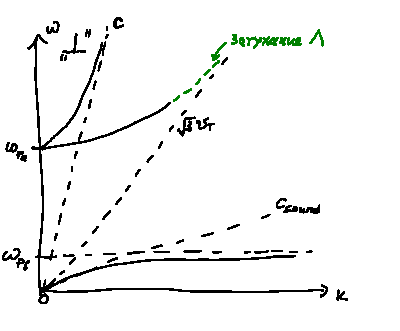
\includegraphics[width=85mm]{noB.pdf}}
    \caption{\label{plot.7.1} Дисперсионка для волн в плазме в отсутствии магнитного поля.}
\end{figure}

Магнитоактивная плазма

Пусть есть внешнее магнитное поле $B_0$, будем рассматривать холодную плазму. Вводя обозначения $n^2=\frac{c^2 k^2}{\omega^2}$, $\upsilon=\frac{\omega_p^2}{\omega^2}$, $u=\frac{\omega_H^2}{\omega^2}$, где $\omega_H$ - циклотронная частота,
дисперсионку можно записать следующим образом:

\begin{equation}
    \label{eq.7.6}
    n_{e,o}^2=1-\frac{2\upsilon (1-\upsilon)}{2(1-\upsilon) - u \sin^2(\theta) \pm \sqrt{u^2 \sin^4(\theta) + 4u(1-\upsilon)^2 \cos^2(\theta)}}, 
\end{equation}
где $\theta$ это угол между магнитным полем и волновым вектором. Индексы e,o соответствуют необыкновенной и обыкновенной волнам.
Cлучай $\theta=0$ представлен на графиках \ref{theta0-u-less-1, theta0-u-more-1}, важно обратить внимание на то, что формула~\ref{eq.7.6} не дает полного решения, нужно ещё учесть $\varepsilon_{\parallel}=0$.

\begin{figure}[h!]
    \center{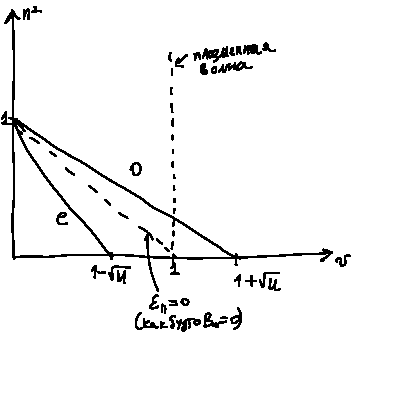
\includegraphics[width=85mm]{theta0-u-less-1.pdf}}
    \caption{\label{theta0-u-less-1} Случай $\theta=0, u < 1$.}
\end{figure}

\begin{figure}[h!]
    \center{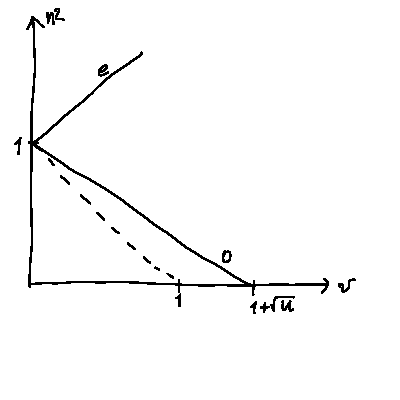
\includegraphics[width=85mm]{theta0-u-more-1.pdf}}
    \caption{\label{theta0-u-more-1} Случай $\theta=0, u > 1$.}
\end{figure}

Теперь расмотрим случай $\theta \ll 1$ (предельного перехода между $\theta=0$ и $\theta \neq 0$, при отсутствии
теплового движения и столкновений нет), дисперсионка в этом случае изображена на рис.~\ref{theta-small-u-less-1, theta-small-u-more-1}. При наличии необнородностей в областях сближения одна волна может переходить в другую.
\begin{figure}[h!]
    \center{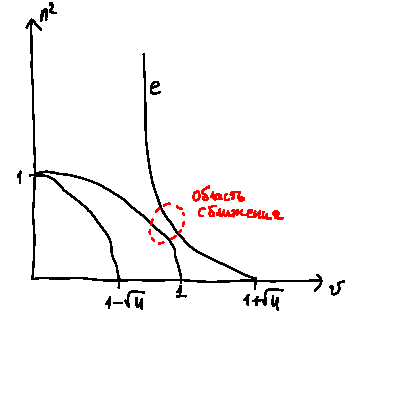
\includegraphics[width=85mm]{theta-small-u-less-1.pdf}}
    \caption{\label{theta-small-u-less-1} Случай $\theta\ll1, u < 1$.}
\end{figure}

\begin{figure}[h!]
    \center{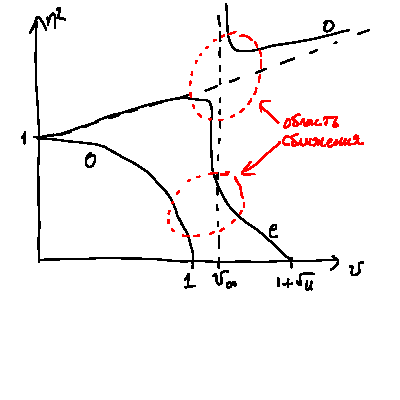
\includegraphics[width=85mm]{theta-small-u-more-1.pdf}}
    \caption{\label{theta-small-u-more-1} Случай $\theta\ll1, u < 1$.}
\end{figure}

Когда $\theta=\pi/2$ график дисперсионка имеет следующий вид~\ref{theta90}.
\begin{figure}[h!]
    \center{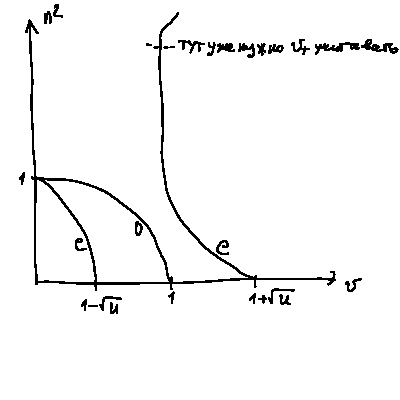
\includegraphics[width=85mm]{theta-90.pdf}}
    \caption{\label{theta-90} Случай $\theta=\pi/2$.}
\end{figure}

Альфвеновские волны. При рассмотрении предыдущих волн, движением ионов принебрегалось. Рассматриваем случай, когда волна распространяется вдоль вшеншего магнитного поля; также рассматриваются низкие частоты (сравнимые с циклотронной частотой ионов ?). Дисперсионка таких волн имеет следующий вид:

\begin{equation}
    \label{alfven}
    \frac{\omega}{k}=\frac{B_0}{\sqrt{4\pi \rho}}
\end{equation}
где $\rho$ есть масстовая плотнотсь плазмы (все частицы). Важно, что фазовая скорость не зависит от частоты! По сути это совместное движение/осцилляции ионов и магных силовых линий поперек движения волны. Они распространяются без дисперсии.

\subsection{Показатель преломления плазмы, пространственная и временная дисперсии, фазовая и групповая скорости плазменных волн.}
\label{sec.7.2}


Диэлектрическая проницаемость в холодной плазме с учетом ионов:

\begin{equation}
    \label{eq.7.7}
    \varepsilon=1 - \frac{\omega_{pe}^2}{\omega^2} - \frac{\omega_{pi}^2}{\omega^2},
\end{equation}
если есть столкновения (пусть отбросим ионы), то $\varepsilon=1-\frac{\omega_{pe}^2}{\omega (\omega+i \nu)}$. когда есть некоторый поток, движущийся со скоростью $\upsilon_0$, то без учета ионов и столкновений, имеем: $\varepsilon=1-\frac{\omega_{pe}^2}{(\omega - k \upsilon_0)^2}$.
Для затухания Ландау: $\varepsilon=1+\frac{4\pi e^2}{m} \int \frac{v}{\omega} \frac{\partial f_0}{\partial v} \frac{dv}{\omega-vk}$.

При наличии внешнего магнитного поля $B_0$ диэликтрическая проницаемость перестает быть изотропной(считаем, что трения нет и $\upsilon_T \ll \upsilon_{ph}$):

\begin{equation}
    \label{eq.7.8}
    \varepsilon=
    \begin{pmatrix}
        \varepsilon_B & ig & 0 \\
        -ig & \varepsilon_B & 0 \\
        0 & 0 & \varepsilon_{\parallel}
    \end{pmatrix}
\end{equation}
 где $\varepsilon_B=1-\frac{\omega_{pe}^2}{\omega^2-\omega_{Be}^2}-\frac{\omega_{pi}^2}{\omega^2-\omega_{Bi^2}}$ и $g=\frac{\omega_{pe}^2 \omega_{Be}}{\omega (\omega^2-\omega_{Be}^2} -\frac{\omega_{pe}^2 \omega_{Be}}{\omega (\omega^2-\omega_{Be}^2}$, $\varepsilon_{\parallel}=1-\frac{\omega_{pe}^2}{\omega^2}-\frac{\omega_{pe}^2}{\omega^2}$. 

Фазовые и групповые скорость изображениы на графиках~\ref{noB} и т.д. Из необычного - фазовая скорость всегда больше скорости света(но это не страшно). 

Пространственная и временная дисперсия(??? общие вещи):
В общем случаем имеем:
\begin{equation}
    \label{eq.7.8}
    \overrightarrow{D}=\iint \varepsilon(t,t',\overrightarrow{r},\overrightarrow{r}') \overrightarrow{E}(t',\overrightarrow{r}') d^3 r' dt,
\end{equation}
в случае однородной и стационарной среды имеем $\varepsilon(t-t', \overrightarrow{r}-\overrightarrow{r}')$, в этом случае
также справедливо $\varepsilon(\omega, \overrightarrow{k})= \varepsilon^*(-\omega, -\overrightarrow{k})$.

\section{Взаимодействие заряженных частиц с волнами в плазме}

\subsection{Возбуждение и затухание волн в плазме, черенковское излучение, затухание Ландау}

\subsection{Раскачка плазменных колебаний пучками}

\subsection{Квазилинейное приближение}

\section{Взаимодействие электромагнитных волн с плазмой}

\subsection{Распространение электромагнитных волн в неоднородной плазме, геометрическая оптика, плазменный резонанс, циклотронный резонанс, линейная трансформация}

\subsection{Основные нелинейные процессы взаимодействия волн, неустойчивость плазмы в сильном электромагнитном поле}

\subsection{Рассеяние и трансформация волн}

\section{Излучение плазмы}
\label{sec.10}
[Котельников, лекции по физике плазмы, глава 7]
В слабоионизированный плазме спектр излучения является линейчатым - за счет молекул, атомов и не полностью ионизованных
ионов. При увеличенни температуры, непрерывный спектр доминирует над дискретным. Полностью ионизованная плазма имеет
непрерывный спектр.
\subsection{Элементарные процессы, интенсивность спектральных линий, сплошные спектры, вынужденное испускание}
\label{sec.10.1}
Можно выделить два типа излучения с непрерывным спектром - тормозное и рекомбинационное; также есть циклотронное,
которое на низких частота имеет линейчатый спектр, а на высоких - становится непрерывм(синхротронное излучение). Однако,
в достаточо плотной плазме циклотронное излучение проглощается и не выходит из плазмы.

Излучение сопровождает переход атома/электрона/иона/молекулы из одного состояния в другое. Есть свободно-свободые переходы
- это есть тормозное излучение (столкновение электронов и ионов) и тормозное поглощение. Связанно-свободные переходы - 
процессы фотоионизации и фоторекомбинации (т.е. освобождение и связывание электрона соотв.). Обы этих типа дают 
непрерывный спектр.

Связанно-связанные переходы электрона между дискретными уровнями энергии приводят в линейчатому спектру. В молекулах также
бывают полосатые спектры - со же самое, но в молекулах бывает, что много уровней рядом образуют совего рода полосу.

\subsection{Пробеги излучения, перенос излучения в среде, оптически прозрачная и непрозрачная плазма, лучистая теплопроводность}
Пробеги излучения -?

\subsubsection{Перенос излучения в среде}
Распространение излученной электромагнитной энергии через некоторую среду может сопровождаться поглощением, излучением и рассеянием. Интенсивность определяется как энергия проходящая в ед. площали $dS$, в ед. $dt$ времени, в ед. $d\omega$ частот:

\begin{equation}
    \label{alfven}
    I_{\omega} = \frac{d\mathcal{E}_{\omega}(\mathbf{r},\mathbf{n},t)}{\cos(\theta)d\omega dSd\Omega dt},
\end{equation}
а уравнение переноса можно записать следующим образом:

\begin{equation}
    \label{alfven}
    \frac{1}{c} \frac{\partial I_{\omega}}{\partial t} + \mathcal{\Omega}\nabla I_{\omega} + (k_s + k_a) I = j_{\omega} + \frac{1}{4\pi} k_s \int I_{\omega} d\Omega,
\end{equation}
где $j_{\omega}$ - коэффициент излучения, $k_s, k_a$ - коэффициенты рассеяния и поглощения. Слагаемое с интегралом имеет смысл излучения рассеянного на поверхность извне.

\subsubsection{Лучистая теплопроводность}

Лучислая или нелинейная теплопроводность - суть в том, что коэффициент теплопроводности зависит от температуры, и уравнение теплопроводности становится нелинейным.


\section{Диагностика плазмы}
\label{sec.11}

Зондовые методы, оптические методы, СВЧ-методы, корпускулярные методы, лазерное рассеяние, магнитные измерения.

\subsection{Зондовые методы}
\label{11.1}

[И.М. Подгорный, лекции по диагностике плазмы, стр. 15]

\subsection{Оптические методы}
\label{11.2}

Определение электронной температуры по интенсивности излучения линейчатого спектра.

При релаксации возбуждённого состояния между уровнями испускается квант с частотой $\nu=\frac{E_2-E_1}{h}$ и интенсивность излучения из объёма будет равна $I=h\nu n_{2} A_{21}$, где $A_{21}$ - вероятность перехода (коэф. Эйнштейна).
\begin{equation}
	n_1 u(v)B_{12}+n_e n_1 <\sigma_1 v>=n_e n_2 (\sigma_2 v) + n_2 A_{21}+n_2 u(v) B_{21}
\end{equation}

, где $n_1$ - концентрация атомов в состоянии 1, $n_2$ - концентрация атомов в сост. 2, $n_e$ - концентрация электронов, $v$ - скорость электронов, $\sigma_1$ эффективное сечение возбуждения, $\sigma_2$ - эффективное сечение, снимающее возбуждение, $u(v)$ спектральная плотность излучения в плазме, $B_{12}, B_{21}$ - коэффициенты эйнштейна. В опытах обычно смотрят на излучение оптически прозрачной плазмы (ничего не поглощает) Есть 2 предельных случая.

\subsubsection{Плазма низкой концентрации}
\label{11.2.1}
Считаем так, если происходит мгновенное высвечивание (пренебрегаем снятие возбуждение ударами)
Уравнение выписывается упрощается до 
\begin{equation}
	n_e n_1 <\sigma_1 v>= n_k  \sum {i=1}{k-1}A_{k i}
\end{equation}
$A_{k i}$ коэффициент эйнштейна для релаксации с уровня k на уровень i.
Следовательно интенсивность излучения 
\begin{equation}
	I=h \nu n_k A_{k1}=h \nu n_e n_1 <\sigma_1 v>\frac{A_{k1}}{\sum{i=1}{k-1} A_{ki}}
\end{equation}

Для резонансной линии отношение $A/\sum A $ равно единице. так же, если мы знаем $n_e, n_i$ и зависимость $<\sigma_1 v>$ от температуры, то можем определить температуру плазмы по отношению относительных интенсивностей двух линий.

\begin{equation}
	\frac{I_1}{I_2}= \ frac {\nu_1 <\sigma_1 v>_1 A_1 \sum A_k^{(2)} }{\nu_2 <\sigma_2 v>_2 A_2 \sum A_k^{(1)} }
\end{equation}
Это самое общее выражение. Далее, можно делать различные предположения (наверное уже не нужно). например, аппроксимировать сечение возбуждения функциями (стр. 45-46).
Не обязательно даже смотреть сваливание на основной уровень.

\subsubsection{Плазма высокой концентрации.}
\label{11.2.2}

Это такая концентрация, что $n_e <\sigma_2 v> \gg A$ 
При выполнения этого условия в отсутствие фотовозбуждения устанавливается между детально обратными процессами $n_1 <\sigma_1 v> = n_2 <\sigma_2 v>$.
Используя известное выражение, для отношений вероятности прямого и обратного процессов:
\begin{equation}
	\frac{<\sigma_1 v>}{<\sigma_2 v>} = \frac{g_1}{g_2} e^{-\frac{E}{kT_e}}
\end{equation}
, где $E$ -  энергия уровня, $g_2$ и $g_1$  - статистические веса соответственно основного и возбуждённого состояний.
В этом случае значение интенсивности спектральной линии, отвечающий переходу из состояния с энергией возбуждения E в основное состояние равно:

\begin{equation}
	I=\frac{h \nu n_1 A g_2}{g_1} e^{-\frac{E}{kT_e}}
\end{equation}
Собственно, отношение двух линий для плазмы высокой концентрации, не зависит от концентрации, а зависит от температуру.
\begin{equation}
	\frac{I_1}{I_2}=\frac{ \nu_1 A_1 g_1}{ \nu_2 A_2 g_2} e^{-\frac{E_1 - E_2}{kT}}
\end{equation}

Т.е. если в эксперименте с электронами распределёнными по больцману измерить интенсивности линий, то можно вывести значение температуры плазмы. 

\subsubsection{определение параметров плазмы по форме спектральных линий}
\label{11.2.3}

Контуры спектральных линий атомов деформируются под действием внешних факторов.
\subsubsection{Определение ионной температуры по доплеровскому уширению спектральных линий}
\label{11.2.3.1}



Из-за допплера длина волны смещается на 
\begin{equation}
	\Delta \lambda = \lambda_0 (1+\frac{v_x}{c})
\end{equation}
Если распределение максвеловское, то  значение составляющей $v_x$  в пределах от  $v_x$  до $v_x + dv_x$ определяется формулой:
\begin{equation}
	\frac{dn}{n}=(\frac{M}{2\pi kT_i})^{1/2} e^{-\frac{Mv^{2}_x}{kT_i}} dv_x
\end{equation}

Из двух этих формул можно получить распределение спектральной плоскости.
\begin{equation}
	I=I_0 e^{-\frac{Mc^{2}}{2kT_i} (\frac{\Delta \lambda}{\lambda_0})^{2}}
\end{equation}

Обычно, определяют полуширину линии. Полуширина линии с температурой связана с температурой.
\begin{equation}
	\delta \lambda_D=\frac{2 \sqrt{2k ln(2)}}{c} \lambda_0 \sqrt{\frac{T_i}{M}}
\end{equation}


\begin{equation}
	T_i(eV)=1.7*10^{8}A(\frac{\delta \lambda_D}{\lambda_0})^{2}
\end{equation}
, где $A$- атомный вес иона.

\subsubsection{эффект доплера на рассеянном свете. Определение электронной температуры.}
\label{11.2.3.2}

Рассмотрим рассеяние монохроматического луча в плазме (оптически тонкой). Если длина волны падающего света много меньше среднего расстояния между заряженными частицами плазмы, а так же меньше дебаевского радиуса, то эффект взаимодействия излучения с плазмой определяется рассеянием на электроне формулой Томпсона: $\sigma =\frac{8\pi}{3} (\frac{e^{2}}{mc^{2}})^{2}$ и для электронов составляет $6.65*10^{-25} cm$.
При работе с плоскополяризованным светом рассеяние не является изотропным и мощность излучения под углом $\theta$ к направлению электрического вектора первичного излучения:

\begin{equation}
	W_{s} (\theta) d\theta=(\frac{e^{2}}{mc^{2}})^{2} W_0 \int {0}{L} n dl cos^{2}(\theta) d \theta
\end{equation}
, где n -  концентрация, а L - путь пучка в плазме.

При максвелловском распределении электронов по скоростям полуширина линии рассеяного света выражается следующим образом.

\begin{equation}
	\delta \lambda_s = 3.3*10^{-3} \lambda \sqrt{T_e (eV)}
\end{equation}
Это можно сделать в предположении не очень большой концентрации, когда лина волны лазера не слишком велика по сравнению с радиусом дебая.
\begin{equation}
	\alpha = \frac{\lambda}{4\pi sin(\frac{theta}{2} \lambda_D)} \ll 1
\end{equation}

, где $\theta$ - угол рассеяния, $lambda_D$ - дебаевский радиус

Это подробно рассмотрено в работе Розенблюта и Ростокера и можно получить окончательное значение для интенсивности света:
\begin{equation}
	I=I_0 exp(- \frac{1}{2} (\frac{\Delta \lambda}{\lambda} \frac{c}{\sqrt{kT_e /m}})^{2})
\end{equation}


\subsubsection{ Штарковское уширение спектральных линий в плазме. определение концентрации ионов.}
\label{11.2.3.3}

В плазме на размерах порядка радиуса дебая, в плазме присутствуют микрополя. Микрополя есть электронные и ионные. Электронные быстро осциллируют, а вот ионные - нет, которые в $\sqrt{M/m}$ раз меньше электронных. Скорости ионов в $\sqrt{m/M}$ раз меньше, то можно полагать, что неподвижный атом находится под быстрым воздействием электронов, находясь в слабоменяющимся поле иона. 

И энергитические уровни возбуждённого атома, находясь под действием этого внешнего электрического поля, расщепляются. А за счёт быстродействующих микрополей электронов, осуществляется переход между штарковскими подуровнями или в результате резкого изменения величины и направления поля происходит сильное изменение фазы излучаемой световой волны. 

Вызванное электронами уширение ОТДЕЛЬНОЙ штарковской компоненты спектральной линии может быть описанной с помощью ударной теории.
\begin{equation}
	I_s=\frac{\gamma}{(\omega + \omega_0 - d)^{2}+ \frac{\gamma^{2}}{4}}
\end{equation}
, где $\omega_0$ - частота линии, $d$ -  смещение линии в электрическом поле
По сути, полуширина линии - обратное время время жизни атома в данном возбуждённом состоянии $\gamma =n_e <\sigma v_e>$.
Сечение электронных столкновений можно записать как $\sigma \sim \pi \rho^{2}$

В квазиклассическом приближении переход из одного возбуждённого состояния в другое под действием столкновений возможен в том случае, есди время пролёта частицы становится сравним с временем перехода между состояниями. В водородном приближении это:
\begin{equation}
	\frac{v}{\rho}=\frac{<d_{m m’}> e}{\hbar \rho^2}
\end{equation}
Здесь $<d_{m m’}>$ - дипольный момент перехода штарковскими коспонентами. записывая его в виде $k^2 a_{0} e$.
Подставляя значение радиуса боровской орбиты приводит, к $\rho \sim \frac{k^2 \hbar}{Zmv}$. Поэтому подставляя это в формулу для сечения получаем, что:
\begin{equation}
	\sigma = \pi k^4 (\frac{h}{mv})^2 Z^2
\end{equation}

В действительности из-за дальнодействуюшего характера дипольного взаимодействия в правую часть этого выражения необходимо добавить множитель $L= ln(\frac{m v_e^{2}}{E-E_1})$ , котрый можно заменить 10.

Критерий применимости ударной теории - длительность столкновений много меньше времени между столкновениями, т.е. $\frac{n^{-1/3}}{v_e} << \frac{1}{n <\sigma v_e>} $ выполняется тем лучше, чем выше концентрация плазмы и чем выше температура.

Так же, данная теория хорошо описывает только хорошо отстоящие от центральной линии (при штарковском уширении происходит разложение несущей спектральной линии)

Для центральной линии это не выполняется (оч маленькие расстояния между подуровнями штарковскими $\omega - \omega_0 <= \gamma$).
Тут вступает в силу теория, которая затрагивает микрополя в плазме, а именно, Хольмарк выдвинул теорию о распределении микрополей в плазме, а именно вероятность поля:
\begin{equation}
	H( \beta ) = \frac{2}{\pi \beta} \int_{0}^{\inf} v sin(v e^{- (\frac{v}{\beta})^{3/2}}) dv
\end{equation}
, где $\beta = \frac{E}{E_0}$ , $E_0 = 2,61 e n^{2/3}$ 
Физический смысл $E_0$ прост: Среднее расположение между частицами плазмы $\frac{1}{n^{1/3}} $, а напряжённость поля точечного заряда обратно пропорциональна квадрату расстояния. Форма функции Хольцмарка:
(нужно картинку).
В этом случае контур линии центральной в рамках применимости запишется как 
\begin{equation}
	I_{st}=\frac{1}{\Delta \omega_0} H(\frac{}{\Delta \omega})
\end{equation}
В этой формуле в случае линейного эффекта Штарка: $\Delta \omega_0 = 2.61 \alpha n^{2/3}$

\subsubsection{Сплошной спектр. определение концентрации и электронной температуры}
\label{11.2.4}
Форма и интенсивность непрерывного спектра излучения плазмы определяется протеканием следующих процессов:
1.Тормозное излучение при взаимодействии электронов с ионами
2.Рекомбинационное излучение, возникающее при радиационном захвате электрона ионом.
3.Тормозное излучение, возникающее в результате электрон-электронных взаимодействий.

Из всех трёх остановимся на первых двух, ибо 3 играет роль в релятивистской плазме и обычно её не наблюдают.

Посмотрим на интенсивность рекомбинационных линий.
\begin{equation}
	I_rec d\nu = A n_i n_e (\frac{E_H}{kT_e})^{3/2} (\frac{E_{ik}}{E_H})^{2} \frac{g_{fb}}{k} \xi_k e^{\frac{(E_{ik}-h \nu)}{kT_e}} d\nu 
\end{equation}
Здесь $E_H = 13.6 eV$ энергия ионизации водорода. $E_{ik}$ - энергия ионизации оболочки, для которой главное квантовое число равно $k$, $g_{fb}$ - множитель Гаунта для свободно-связанных переходов.$ \xi_k$ - число квантовых мест на $k$-ой оболочке (если пустая, то $ \xi_k = 2k^{2}$ ). 
Видно, что мощность рекомбинационного излучения пропорциональна $Z^{4}/k^3$
Видно, что этот спектр имеет РЕЗКУЮ границу. Нету фотонов с энергией меньше чем $E_{ik}$, а с другой стороны есть длинный хвост, который описывается степенью экспоненты делённую на температуру. По этому хвосту и можно восстановить температуру

\begin{figure}[h!]
	\center{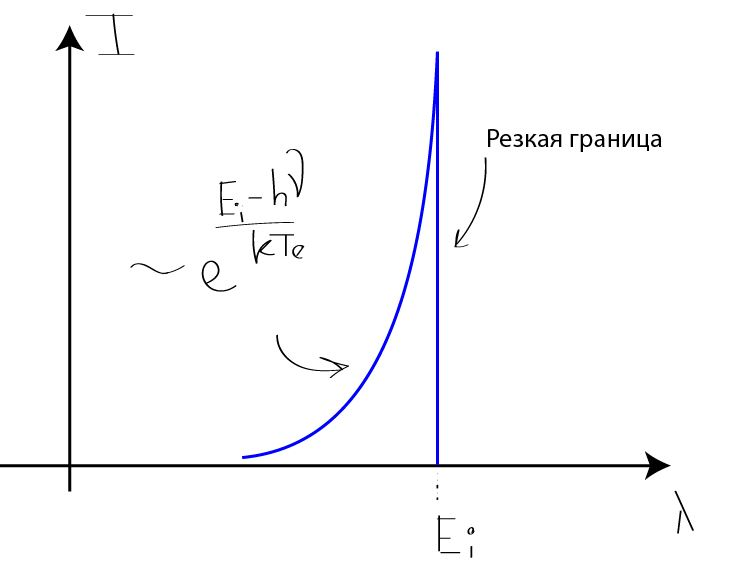
\includegraphics[width=70mm]{Intencity_recomb.JPG}}
	%\caption{\label{fig.2.4.1}}
\end{figure}

В случае тормозного излучения, обусловленного свободно-свободными переходами, в отличие от рекомбинационного, неограниченно простирается в сторону длинных волн. Мощность излучения в единице объёма плазмы в телесном угле $4 \pi$ , приходящийся в интервал частоты $d\nu$.

\begin{equation}
	I_torm d\nu = A Z^{2} n_i n_e (\frac{E_H}{kT_e})^{1/2} e^{-\frac{h \nu}{kT_e}} g_{ff} d\nu
\end{equation}
, где $g_{ff}$ множитель граута, который в широком диапазоне температур имеет сложный характер, но он порядка 1.

В общем, если смотреть на мощность излучения, то она для тормозного излучения будет:
\begin{equation}
	Q_torm=1.5 *10^{-25} Z^{2} n_e n_i T^{1/2}[eV]
\end{equation}
\begin{equation}
	Q_rec=5 *10^{-24} Z^{4} n_e n_i T^{-1/2}[eV]
\end{equation}

Видно, что для водородоподобной плазмы, они сравниваются для энергий 30eV. Свыше 100ev основной вклад в континуум даёт тормозное излучение.

\subsubsection{Сплошной спектр. ИК область}
\label{11.2.5}

Он интересен тем, что измерения проводятся в большом диапазоне энергий. Можно мерить и концентрацию и эл. температуру.
Необходимо выбрать такой участок спектра, внутри которого происходит переход от объёмного тормозного спектра излучения к поверхностному.
Поверхностное излучение отвечает случаю отвечает излучению чёрного тела и реализуется для слабого поглощения в плазме. Мощность излучения чёрного тела зависит только от температуры, то есть измерив его мощность - определим температуру.

По скольку в широкой области концентраций и электронных температур самопоглощение ИК излучение можно не учитывать, концентрация плазмы связана с температурой электронов формулой:
\begin{equation}
	n=3.9*10^{19} T_e^{\frac{1}{4}}[eV] (\frac{\int_{\Delta \nu g_{ff}} I(\nu) d\nu}{\Delta \nu g_{ff}})^{\frac{1}{2}}   cm^{-3}
\end{equation}

\subsubsection{Определение диэлектрической проницаемости плазмы. СВЧ метод}
\label{11.4}

Вспоминаем, что распространение ЭМ волн в плазме определяется диэлектрической проницаемостью.
\begin{equation}
	\epsilon = 1- \frac{\omega_{pl}^{2}}{\omega^{2}} \frac{1}{1-i \frac{\nu_{collision}}{\omega}}
\end{equation} 
, где $\nu_{collision}=\frac{2*10^{-5} n_i Z}{T_e^{3/2}[eV]}$, $\omega$ - частота волны

В случае малого поглощения, убирается мнимая часть.
\begin{equation}
	\epsilon = 1- \frac{\omega_{pl}^{2}}{\omega^{2}} 
\end{equation} 
Тоесть, если мы сможем измерить эпсилон для среды и конкретной частоты - узнаем и $\omega_pl = \sqrt{\frac{4 \pi e^{2} n_e}{m}}$, то узнаем концентрацию $n_e$

То есть что делают, берут какой-то СВЧ генератор, светят на плазму. Если проходит, значит концентрация меньше критической для данной частоты. Если отражается назад, то значит внутри есть слой с критической концентрацией. Это метод отсечки.
Оправданно это при условии $l \gg \frac{c}{\omega_pl}$
, где $l$ - толщина слоя плазмы с концентрацией выше критической, $\omega_pl$ - плазменная частота.

Если такой слой достаточно мал, то прибегают к интерферометрии. Собирают установку, где часть СВЧ сигнала проходит по участку, занятому плазмой, половина по свободному тракту. Далее, сигналы суммируют в интерферометре. По амплитуде суммарного сигнала, можно судить о разности фаз.
 
\begin{figure}[h!]
	\center{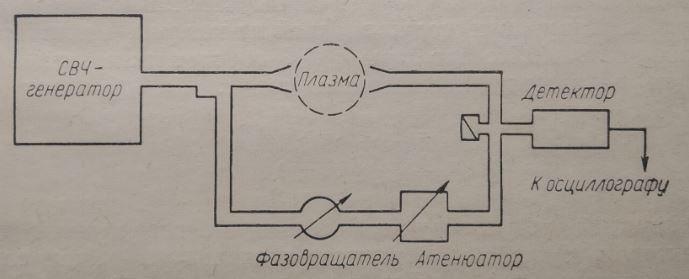
\includegraphics[width=70mm]{HF interferometre.JPG}}
	%\caption{\label{fig.2.4.1}}
\end{figure}
 
 Очевидно, что разность фаз - набег фазы по пути через плазму с коэффициентом преломления N.
 \begin{equation}
 	\phi = \frac{2 \pi}{\lambda} \int_{0}^{l} [N_0 - N(x)] dx 
 \end{equation} 
, здесь $l$ - размер плазмы, $N=\sqrt{\epsilon}$ - показатель преломления, $\lambda$ - длина волны СВЧ. Вообще, если тракт откачан воздухом, то $N_0 =1$


\subsubsection{Определение диэлектрической проницаемости плазмы. Применение лазеров}
\label{11.5}
Когда частоты СВЧ не хватает, для большой концентрации плазмы, используют лазеры.
Принцип абсолютно тот же, лазерный пучок пропускают через плазму и интерферируют самим с собой. На экране камеры получают интерфериционную картинку в виде полос. Потом, когда на пути пучка возникает плазма, в тех местах где увеличена концентрация, там уменьшается показатель преломления среды и как следствие, интерференционная картина превращается в кривые полосы. По кривизне полос в каждой точке, можно судить о набеге фаз.

\subsubsection{Корпускулярные методы диагностики плазмы}
\label{11.6}

\subsubsection{Использование пучков заряженных частиц}
\label{11.6.1}
С помощью пучка можно исследовать оч быстрые изменения плазмы. Конфигурации эксперимента оч разные, поэтому приводятся лишь некоторые из них.
Первое это зондирование пучком плазмы для определения радиальной и азимутальной компоненты поля в магнитной ловушке. Двигаясь продольно магнитному полю, при наличии поперечного поля электроны будут испытывать дрейф в скрещенных полях. Помещая электронную пушку в области одной пробки, люминисцентный экран в другой пробке, можем вижеть отклонение эл пучка на экране.
В отсутствие плазмы пучок двигается вдоль линий магнитного поля и делает точку на люминофоре. Наличие дрейфового движения приводит к смещение на экране на расстояние
\begin{equation}
	\Delta x=\frac{cE_y}{H_z} * \frac{l}{v}
\end{equation}
. где $l$ - длина пути пучка в плазме, $E_y$ - составляющая электрического поля, перпендикулярная магнитному полю, $v$ - скорость движения электронов вдоль линий поля.
Соответственно, смещение по радиусу пучка это азимутальная компонента поля, смещение по углу - радиальная компонента поля E.

Для определения потенциала плазмы относительно стенок используют метод, основанный на запирании пучка электронов. Время пролёта через плазму:
\begin{equation}
	\tau = \sqrt{\frac{M_i}{2Z_i}} \int_{0}^{l} \frac{dx}{\sqrt{V_0 +V(x)}}
\end{equation}
, где $Z_i$ - заряд иона.$M_i$ - масса иона, $l$ - размер плазмы, $V_0$ ускоряющий потенциал в источнике ионов, $V(x)$ - распределение потенциала вдоль пути пучка.
Если падение потенциала почти всё сосредоточено в дебаевском рабиусе, значительно меньшим $l$, то выражение будет
\begin{equation}
	\tau = \frac{l}{v_i}
\end{equation}
, где 
\begin{equation}
   v_i= sqrt{\frac{Z_l (V_0 + V_pl)}{M_i}}
\end{equation}

Область применимости- не должны влиять неустойчивости. Время прохождения через плазму должно быть меньше, чем время развития неустойчивостей.
\begin{equation}
	\tau_{neust} =(\frac{n}{n'})^{1/3} \frac{1}{\omega_{pl}}
\end{equation}
, где $n'$ - концентрация электронов в пучке.




\subsubsection{Измерение концентрации нейтральных и заряженных частиц.}
\label{11.6.2}

Прохождение пучка атомов или ионов через плазму сопровождается атомными и электронными столкновениями, приводящие к изменению заряда пучка. И то, на сколько он потеряет заряд - тоже будет функция температуры и концентрации электронов.
Рассмотрим изменение зарядового состояния монохроматического атомного пучка, состоящих из нейтральных атомов и протонов водорода, при прохождении через водородную плазму.
Средне квадратичный угол отклонения пучка будет:
\begin{equation}
 \overline{\theta} = 2 (\frac{Z_1 Z_2 e^{2}}{M v^2}) \sqrt{2 \pi nLl}
\end{equation}
, где $l$ - длина пути пучка в плазме с концентрацией $n$, $L$ - кулоновский логарифм ($L \sim 15$); $M$ - масса частицы пучка.
Для водорода с энергией электрона $10^{4} eV$ для $nl \sim 3*10^{16}$ среднеквадратичный угол будет $1.5^{\circ}$ 
Основные элементарные процессы плазмы с пучком.
1. Захват быстрым протоном электрона при взаимодействием с нейтральными атомами плазмы.
2. Обдирка электрона, принадлежащему быстрому атому, при взаимодействии его с нейтральными атомами среды.
3. Обдирка электрона, принадлежащему быстрому атому на протонахх плазмы.
4. Ионизация быстрых атомов электронами плазмы. 
Для описания каждого процесса, по факту пишут баланское уравнение по трассе пучка:
\begin{equation}
	\frac{dN_0}{dl} = -N_0 n_0 \sigma_{01}-N_0 n_i \sigma_{10} 
\end{equation}
и т.п., решаем с граничными условиями, сравниваем с экспериментом, делаем предположения о температуре плазмы и концентрации. Непосредственно сам пучок измеряется с помощью масс-спектрометров.


\subsubsection{Масс-спектроскопическая методика исследования быстрых частиц плазмы}
\label{11.6.3}

 Пучок, выходящий из плазмы, направляется в магнитное поле. В зависимости от массы и заряда, все частицы отклоняются на разные углы. Приближённо, отклонение на экране регистратора можно записать как
 
 \begin{equation}
 	x=\frac{ZeHl^{*}h}{Mv}
 \end{equation}
, где $l^{*}$ - расстояние между магнитом и детектором, $h$- протяжённость магнитного поля

\subsubsection{Калометрические измерение плазмы}
\label{11.6.4}
Есть несколько измерений.
1. Определение кривой распределения потоков тепла на стенку в относительных единицах.
2. определение энергии на данный участок поверхности.
3. Определение временного хода тепла.


Проще всего 1-я задача. Если на единице поверхности теплообменника выделяется количество тепла в Q калорий, то увеличесние его температуры определяется формулой.
 \begin{equation}
	\Delta \theta= \frac{Q}{dch} (1-\gamma)
\end{equation}
Здесь $d$ - плотность, $c$ - теплоёмкость и $h$ - толщина теплоприёмника, а $\gamma$ коэффициент отражения плазмы (обычно равен десятку процентов)
Вообще для измерения используют балометры. Так же можно исследовать мощность в зависимости от времени.
 \begin{equation}
	\Delta \theta= \int_{0}^{t} \frac{1}{dch} \frac{dQ}{dt}
\end{equation}

\subsubsection{Регистрация жёстких излучений плазмы}
\label{11.6.5}
Используют метод наведённой радиоактивности для того, чтобы обнаружить и измерить нейтронные импульсы интенсивности $10^4 - 10^5$ нейтронов и выше.
В естественном серебре есть два изотопа. $Ag^{107} Ag^{109}$ примерно в равных количествах. Сечения захвата 44 и 110 Барн соответственно. В следствие захвата образуются  $Ag^{108} Ag^{110}$ с периодом полураспада 2,4мин и 24,5сек, которые испытывают $\beta$ распад, который можно регистрировать. Собственно минимальная длительность определяется именно минимальным полураспадом, скважность между ними - максимальным временем полураспада.
Следующий метод - сцинтиляторный регистратор. ЧТо это такое. Ставят условный "друшлаг" - экран с большим количеством дырочек, за которым есть флуорисцирующий экран. Пучок нейтронов пролетает в дырки на друшлаге и попадают на экран, но из-за разлёта по углу, расстояние между светящимися точками на экране не такое как на друшлаге.

\begin{figure}[h!]
	\center{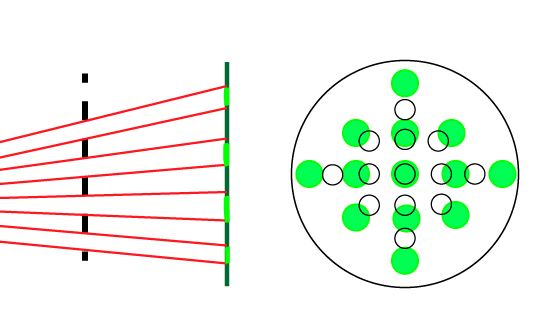
\includegraphics[width=70mm]{scintelator.JPG}}
	%\caption{\label{fig.2.4.1}}
\end{figure}

Так же используют Камеру обскура и Камеру Вильсона.

\section{Электрический разряд в газах}

\subsection{Основные виды разряда: тлеющий разряд, искра, электрическая дуга, ВЧ-, СВЧ-и оптический разряд}
\subsubsection{Тлеющий разряд}
Характеризуется не очень большим током, малыми давлениями.
Быстрее всего описан: [Сивухин, общий курс физики, 3 том., параграф 117]
\begin{figure}[h!]
	\center{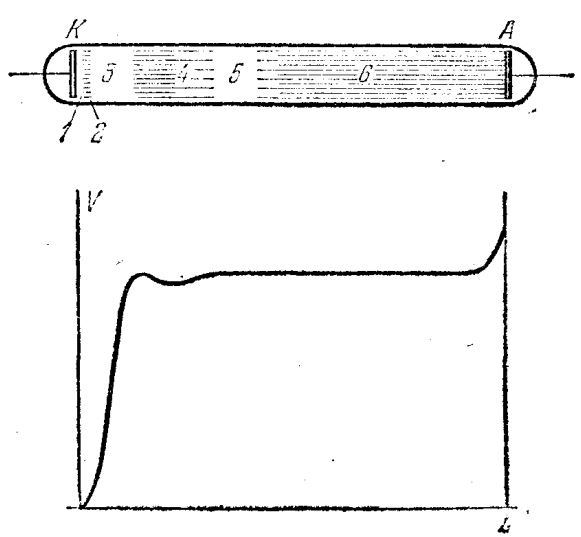
\includegraphics[width=70mm]{12.1.JPG}}
	%\caption{\label{fig.2.4.1}}
\end{figure}
Область 1 - область эмиссии электронов. 2 - катодный слой, идёт возбуждение нейтралов электронами, 3 - тёмное катодное пространство, область где происходит первичная ионизация, тут происходит затравка электронной лавины 4 - область рекомбинации ионов, идущих справа, и электронов, идущих слева. 5 - тёмное андоное пространство - ионов не так много, электроны ещё не успели снова набрать скорость. Все предыдущие области отвечали за поддержание лавины. Именно они определяют её существование  6 - положительный андоный столб/анодное свечение, в основном вызванное рекомбинацией электронов с ионами, которые были образованы на расстоянии нескольких пробегов до анода. Область эта характеризуется высоким зарядовым числом ионов, высокой проводимостью.
\subsubsection{искровой разряд}
[Сивухин, общий курс физики, 3 том., параграф 118]

Характеризуется большими давлениями и большим напряжением пробоя.
Имеет ломанную форму, так как в следствие первичного пробоя стримером, возникает канал ионизации, по которому начинает течь ток огромный ток, который вслед за собой вызывает возбуждение и свечение в УФ диапазоне. Вблизи канала УФ излучением ионизуются новые молекулы, которые становятся затравками для новых искр. Поэтому, форма очень ветвистая.

\subsubsection{коронный разряд}
[Сивухин, общий курс физики, 3 том., параграф 119]
Возникает при больших давлениях в сильно неоднородных полях (острия игл). В зависимости от напряжения на игле может быть 2 разных разряда. С положительной короной и отрицательной.
У отрицательной короны положительные ионы образуются электронными лавинами, которые были ускорены в области неоднородного поля катода. Ионы попавшие на катод, выбивают ещё электронов.
В случае положительной короны,  электронные лавины пораждаются фотоионизацией самой же короны.

\subsubsection{дуговой разряд}
[Сивухин, общий курс физики, 3 том., параграф 120]
Характеризуется большим током, малым напряжением, большими давлениями.
После первичного пробоя газа, по каналу начинает бежать большой ток. Сопротивление канала резко падает. Из-за большого тока, электроны с собой захватывают и часть электродов. тем самым, лавина поддерживается термоэмиссией заряженых частиц с электродов.

\subsubsection{ВЧ разряд}
[райзер Ю.П., лазерная искра и распространение разрядов, гл 7, пар 28]
До этого всё были пробои в относительно стационарных полях, но для разряда это вовсе не обязательно. Большая напряжённость эл поля может быть достигнута и другими способами. Например, собирается колебательный контур с большими конденсаторами и катушкой. Конденсаторы сначала заряжаются, а потом замыкаются через катушку (индуктор). В катушке подскакивает ток, как следствие внутри возникает большое магнитное поле, которое порождает электрическое, которое в свою очередь вызывает разряд.
\begin{figure}[h!]
	\center{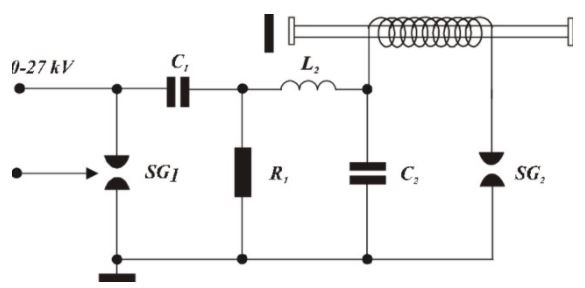
\includegraphics[width=70mm]{12.5.JPG}}
	%\caption{\label{fig.2.4.1}}
\end{figure}
на рисунке приведена схема лазера, активная область которого создаётся индукторным разрядом.
В том случае, если у нас не импульсно будет происходить разрядка конденсаторов, а мы будем поддерживать колебания в этом контуре, то это будет ВЧ разряд индукционного типа.
[райзер, физика газового разряда, 3-е изд, глава 18.2]
Так же есть ВЧ разряд ёмкостного типа. Внутри конденсатора создаётся область переменного электрического поля. Которую можно рассматривать как конденсатор с проводимостью. И из-за этого ток может быть смещён по фазе, относительно внешнего напряжения, что ограничивает мощность.
\subsubsection{СВЧ разряд}
Переменное в пространстве поле можно создавать вообще без электродов, например СВЧ пучком. Так как энергия кванта СВЧ излучения мала, то ясно что “нагрев” (набор энергии электронов) происходит на столкновениях,  так как если бы вообще не было столкновений, то электрон бы энергию в переменном поле не набирал. Понятно, что чем больше поле, тем быстрее электрон в нём набирает энергию, однако у нас появляется поправка, связанная с частотой соударений, а именно если вспомнить “нагрев на столкновениях” то там можно ввести эффективное поле греющее поле $E_{eff}=E \frac{\nu_{tr}^{2}}{\nu_{tr}^{2}+\omega^{2}}$. 
\subsubsection{Лазерный разряд / лазерная искра}
[райзер Ю.П., лазерная искра и распространение разрядов, гл 1, пар 1]
Тут основным механизмом создания плазмы разряда естественно тоже будет ионизация. Однако она может иметь двух видов. 1) нагрев на столкновениях (в достаточно большом поле, ИК область) 2) фотоионизация (многоквантовый процесс при большой интенсивности света и большой энергии кванта)

\subsection{Условия стационарности разряда, излучающий разряд в плотной плазме, плазменно-пучковый разряд}
\subsubsection{Условие стационарности разряда}

Вообще, условие стационарности ЛЮБОГО разряда,  это частота рождения электронов должна быть равна частоте их гибели. $\nu_{born} = \nu_{death}$ . Рождение электронов - инонизация любых видов, отлипание от отрицательного иона. Гибель - диффузия всех видов, рекомбинация, так же туда относят потери энергии на возбуждение частиц, хотя электроны непосредственно не теряются, но они теряют энергию. Тем самым, замедляется рост электронной лавины. 

\subsection{Излучение разряда в плотной плазме}

?
ну понятно, что в разряде будут возбуждаться молеулы, будет происходить рекомбинация. Понятно, что все эти линии будут видны. В случае равновесного разряда ($T_e = T_i$), у нас будет ещё и излучение чёрного тела.

\subsection{Плазменно-пучковый разряд}

Плазменно-пучковый разряд - один из видов электрич. разрядов в газе, при котором в межэлектродное пространство вводится ускоренный пучок электронов и плазма разряда разогревается гл. обр. за счёт пучковой неустойчивости. В результате развития неустойчивости ср. энергия электронов в пучке уменьшается, часть энергии пучка передаётся ленгмюровским волнам, которые затем передают её тепловым электронам плазмы. Разогрев тепловых электронов происходит за счёт затухания ленгмюровских волн при столкновениях, при их рассеянии на тепловых электронах с трансформацией ленгмюровских волн в ионнозвуковые и т. д.
Доля $\alpha$ энергии пучка, трансформируемая в энергию ленгмюровских волн, зависит от первоначального разброса скоростей электронов пуч­ка и от длины взаимодействия пучка с плазмой. Наибольшие значения $\alpha$  (порядка 1) реализуются для пучка, достаточно размытого по скоростям.
В П.п. р. значит. вклад в ионизацию вносят разогретые тепловые электроны плазмы, концентрация которых по мере развития разряда обычно начинает превышать концентрацию электронов в пучке. На формирование функции распределения тепловых электронов оказывают влияние упругие и неупругие столкновения, а так­же ускорение электронов в электрич. полях ленгмюровских колебаний.


\section{ Гидродинамические и тепловые явления в плазме}
\label{13}

\subsection{Ударные волны в плазме}
\label{131}
[Зельдович Райзер, Физика ударных волн и ….. стр. 398]
Плазма характеризуется двумя температурами, электронной и ионной. Каждая может быть иногда описана максвеллом. Если меняется какой либо параметр, то характерное время максвеллизации составляет порядка времени столкновения $\tau_{collision}$. С температурами всё гораздо труднее, если одна из них изменилась, то вторая изменится за достаточно большое время, порядка $\tau_{ei}=\sqrt(\frac{M}{m}) \tau_{collision i}$ (передаётся малая часть энергии от электрона к иону). То есть, температура устанавливается не мгновенно.
Теперь рассмотрим ударную волну, летящую по ионизированному веществу.
На границе раздела двух плотностей и температур есть разрыв. Проходя по веществу, волна в области фронта разогревает ионы (как и нейтралы) в соответствие с показателем адиабаты $\gamma$ (для водородной плазмы 5/3). Так как в фронте создалось уплотнение ионов, они подтягивают за собой электроны, при чём это оч быстро происходит, так как плазма в целом квазинейтральна становится быть. Однако температура электронов из-за такого сжатия увеличивается всего лишь в $4^{\gamma - 1}=2,5$ раз. А выравнивания температуры с ионами не происходит, из-за медленности процесса, поэтому и могут реализоваться случаи, когда за границей разрыва температуры электронов и ионов сильно отличаются. Характерное расстояние, на котором они ещё разные $\Delta x = u_1*\tau_{ei} =u_1* \sqrt(\frac{M}{m}) \tau_{collision}$
\begin{figure}[h!]
	{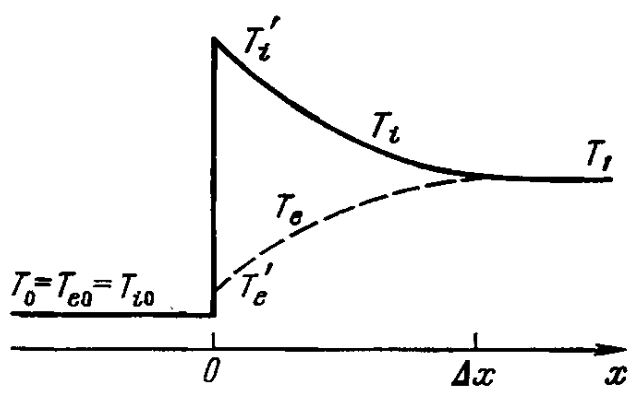
\includegraphics[width=70mm]{13. Skach plotn.JPG}}
	%\caption{\label{fig.2.4.1}}
\end{figure}
так же, поскольку электроны являются быстрыми, то они хорошо переносят температуру. Коэффициент температуропроводности для них будут порядка: $\chi \sim l\bar{v}$ из-за сечений и масштаб длины порядка длин пробега $\lambda \sim \chi /D \sim l \bar{v}/D \sim l$
Коэффициент температуропроводности равен:
\begin{equation}
	\chi_e=\frac{l_e \bar{v_e}}{3} \approx \frac{\bar{v_e^{2}} \tau_e}{3}
\end{equation} 
где $l_e$ длина пробега электронов, $\bar{v_e}$ - их тепловая скорость, а $tau_e$ - время между столкновениями электронов друг с другом.
Как было показано ранее, длина пробега заряженых частиц не зависит от их массы, а зависит только от заряда и температуры $l \sim \frac{T^{2}}{Z^{4}}$. Для водородной плазмы (Z=1) длины пробега электронов одного порядка, однако, скорость электронов больше в $\sqrt{m_i / m_e}$ раз больше чем ионов. Поэтому и коэффициент теэлектронной теплопроводности и характерный масштаб, на которой разыгрывается процесс электронной теплопроводности:
\begin{equation}
	\lambda_e \sim \frac{\chi_e}{D} \sim \sqrt{\frac{m_i}{m_e}} \frac{\chi_i}{D} \sim \sqrt{\frac{m_i}{m_e}} l_i
\end{equation}
Этот маштаб такого же порядка, что и ширина релаксационной зоны выравнивания температур электронного и ионного газов:
\begin{equation}
	\Delta x \sim D \tau_{ei} \sim D \sqrt{\frac{m_i}{m_e}} \tau_i \sim \frac{D}{\bar{v}} \sqrt{\frac{m_i}{m_e}} l_i \sim \sqrt{\frac{m_i}{m_e}} l_i
\end{equation}

Поэтому по отношению к электронной теплопроводности градиенты в релаксационной зоне не малы и теплопроводностный теплообмен в этой зоне сравним с теплообменом между ионами и электронами. Электронная теплопроводность способствует скорейшему выравниванию температур за вязким скачком, так как она перекачивает тепло из более удаленных от скачка уплотнения слоев газа в передние, где электронная температура меньше. 
рассмотрим теперь на сколько глубоко проникает тепло перед скачком уплотнения.
Для этого запишем поток электронной тепропроводности:
\begin{equation}
	S=-\kappa_e \frac{dT_e}{dx}=-\chi_e c_e \frac{dT_e}{dx}
\end{equation}
, где $\kappa_e = \upchi_e c_e$ - коэффициент температуропроводности, $c_e$ теплоёмкость 1см3 электронного газа при постоянном объёме.
Вообще, эффективный коэффициент электронной теплопроводности равен:
$\kappa_e = \xi \frac{(kT_e)^(5/2) k}{m_e^{1/2} Z e^{4} ln(\Lambda)} = \xi *1.93*10^{-5}\frac{T^{5/2}}{Z ln|Lambda} $ эрг/сек*см*град
, где $ln\Lambda$ - кулоновский логарифм, а $\xi$ -число слабо зависящее от Z.
В силу стационарности процесса поток теплопроводности в прогревном слое равен гидродинамическому потоку электронной энергии.
\begin{equation}
	-S= D c_e T_e = \upchi_e c_e \frac{dT}{dx}
\end{equation}
(начальная температура электронов перед фронтом предполагается равной нулю; далеко перед волною поток S исчезает)
Замечая, что $\chi_e \sim \bar{v_e} \sim T_e^{5/2} $, или полагая $\chi_e=\alpha T_e^{5/2}$. Тогда интегрируем выражение и получим, что:
\begin{equation}
	x-x_0 = \frac{2}{5} \frac{a}{D} T_e^{-5/2}
\end{equation}
Или 
\begin{equation}
	T_e = [\frac{5}{2} [\frac{D}{a} (x-x_0) ]^{2/5}
\end{equation}
, где $x_0$ координата, где температура обращается в 0. Всё это изображено на рис ниже.

\begin{figure}[h!]
	\center{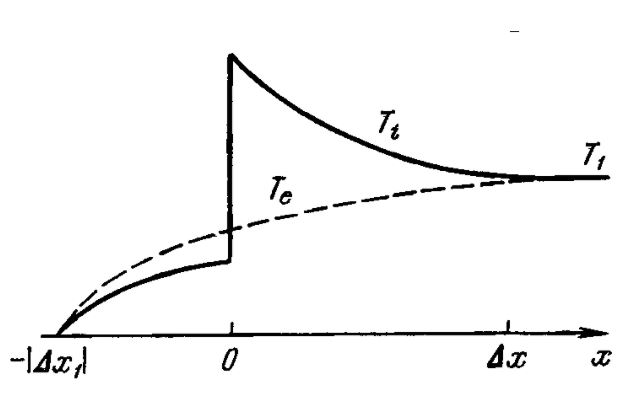
\includegraphics[width=70mm]{13. teploprov.JPG}}
	%\caption{\label{fig.2.4.1}}
\end{figure}

Скачок уплотнения [Зельдович Райзер, Физика ударных волн и ….. стр. 362]


Именно благодаря вязкости осуществляется необратимое превращение в тепло значительной части кинетической энергии газодинамического потока, набегающего на разрыв в системе координат, где разрыв покоится. 
Поскольку процесс ударного сжатия в скачке уплотнения разыгрывается на расстояниях, соизмеримых с газокинетическим пробегом молекул, при изучении структуры скачка следовало бы, строго говоря, исходить из представлений молекулярно-кинетической теории газов. 
Запишем уравнения одномерного течения вязкого и теплопроводного газа, стационарного в системе координат, связанной с фронтом волны: 

\begin{eqnarray}
	\frac{d}{dx} \rho u =0 \\
	2 \rho u \frac{du}{dx} + \frac{dp}{dx}-\frac{d}{dx} \frac{4}{3} \mu \frac{du}{dx} =0 \\
	 \rho uT \frac{d \sum}{dx}=\frac{4}{3} \mu (\frac{du}{dx})^{2} - \frac{dS}{dx}
\end{eqnarray}
, где $\sum$ - удельная энтропия, $\mu$  - коэффициент вязкости, $S$ - негидродинамический поток энергии, равный в случае теплопроводности $S=-\kappa \frac{dT}{dx}$ , где $\kappa$ - коэффициент теплопроводности.
Преобразуя третье уравнение G.1) с помощью второго закона термодинамики: 
\begin{equation}
	T \sum = d \epsilon + p dV = dw  - \frac{1}{\rho} dp 
\end{equation}
И интегрируя все уравнения получем первые интегралы системы:
\begin{eqnarray}
	\rho u = \rho_0 D \\  p+\rho u^{2} - \frac{4}{3} \mu \frac{du}{dx} = p_0 + \rho_0 D^{2} \\  w + \frac{u^{2}}{2} + \frac{1}{\rho_0 D} (S - \frac{4}{3} \mu u \frac{du}{dx}) = w_0 + \frac{D^{2}}{2}
\end{eqnarray}
Если подставить крайние значения и невозмущённые концентрации, то это будет прямо законы сохранения. 
Из этих соотношений следует, что скачок энтропии в ударной волне $\sum_1 - \sum_2 = \sum (p_1, \rho_1) - \sum (p_0, \rho_0)$  совершенно не зависит ни от механизма диссипации, ни от величины коэффициентов вязкости $\mu$ и теплопроводности $\kappa$. Они лишь определяют его толщину.
Вводится безразмерная величина $\eta = \frac{\rho_0}{\rho} $
И так же получается, что
\begin{equation}
	\frac{p}{p_0}=\frac{1 + \frac{M^{2}}{3} (1-\eta^{2})}{\eta}=\frac{4 \eta_1 - \eta^{2}}{(4 \eta_1 -1) \eta}
\end{equation}
где, $\eta_1 = \frac{1}{4}+\frac{5}{4} \frac{p_0}{\rho_0 D^{2}}=  \frac{1}{4} + \frac{3}{4} \frac{1}{M^{2}}$

где, $M=\frac{D}{c_0}$ - число Маха, $c_0$ - скорость звука в начальном состоянии 
Подставляя это всё в систему, получим дифференциальное уравнение:
\begin{equation}
	\frac{5}{3} \frac{\mu}{\rho_0 D} \eta \frac{d\eta}{dx}=-(1-\eta)(\eta - \eta_1)
\end{equation}
\begin{figure}[h!]
	\center{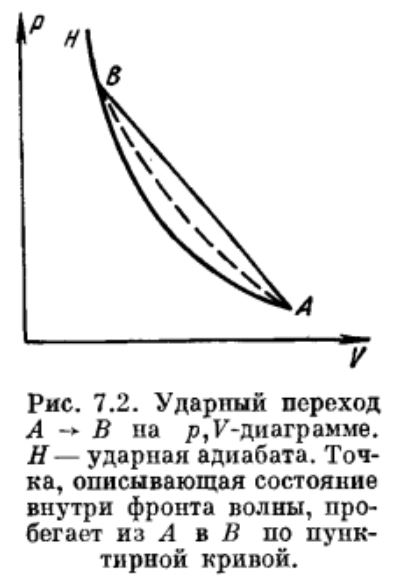
\includegraphics[width=70mm]{13. adiab udarn.JPG}}
	%\caption{\label{fig.2.4.1}}
\end{figure}
Оценим ширину фронта как:
\begin{equation}
	\delta = \frac{D-u_1}{(\frac{du}{dx})_{max}}
\end{equation}
По порядку она будет:
\begin{equation}
	\delta \sim l_0 \frac{M}{M^{2}-1}
\end{equation}
Применима до тех пор, пока $\delta$ больше $l$. например, $M=2$ то $\delta=3 l$.
Роли вязкости и теплопроводности в образовании скачка уплотнения 
Если не учитывать вязкости, то первые интегралы уравнений гидродинамики одномерного стационарного течения G.3) принимают вид: 

\begin{eqnarray}
	\rho u = \rho_0 D \\ p+\rho u^{2} - \frac{4}{3} \mu \frac{du}{dx} = p_0 + \rho_0 D^{2} \\ w + \frac{u^{2}}{2} + \frac{S}{\rho_0 D}  = w_0 + \frac{D^{2}}{2}
\end{eqnarray}
Из первых двух уравнений G.10) следует, что в процессе ударного сжатия в отсутствие Вязкости состояние частицы газа должно непрерывным образом меняться вдоль прямой на диаграмме давление — удельный объем. 
\begin{eqnarray}
	p=p_0 + \rho_0 D^{2} (1-\eta) \\ \eta=\frac{V}{V_0}
\end{eqnarray}
Это важное свойство течения невязкого газа иллюстрируется рис. 7.4, на котором изображена ударная адиабата и прямая, связывающая начальное и конечное состояния газа. Попытаемся решить систему уравнений: 

\begin{equation}
	\frac{T_1}{T_0}=1+ \frac{2 \gamma (\gamma-1)}{(\gamma+1)^{2}} (M^2-1)(1+\frac{1}{\gamma M^{2}})
\end{equation}


Релаксационный слой [Зельдович Райзер, Физика ударных волн и ….. стр. 362]
Для возбуждения некоторых степеней свободы газа *) часто требуется много соударений молекул, причем необходимые числа соударений, т. е. времена релаксации, для разных степеней свободы могут сильно различаться. 
Время установления полного термодинамического равновесия во фронте ударной волны, а следовательно, и ширина фронта определяются наиболее медленным из релаксационных процессов. При этом, конечно, следует принимать во внимание только те процессы, которые приводят к возбуждению степеней свободы, дающих заметный вклад в теплоемкость 
при конечных параметрах газа. Если тшах — наибольшее время релаксации, а щ — скорость движения газа за фронтом относительно самого фронта, то ширина фронта порядка $\Delta x \sim u_1 \tau_max =D(\rho_0 / \rho_1) \tau_max$.

При комнатных температурах вращения в молекулах возбуждаются также быстро, в результате небольшого числа соударений; колебания же при этих температурах обычно не играют роли. Следовательно, ширина фронта слабых ударных волн, распространяющихся по молекулярному газу, нагретому до комнатной температуры, порядка нескольких газо-кинетических пробегов. 

При температурах порядка 1000° К, когда величина кТ сравнима с энергией колебательных квантов молекул $h\nu_osc$, возбуждение колебаний требует многих тысяч, а иногда десятков и сотен тысяч соударений. Ширина фронта ударной волны соответствующей амплитуды определяется временем релаксации для колебательных степеней свободы. 
Диссипативные процессы — вязкость и теплопроводность — играют роль только в области больших градиентов гидродинамических величин, т. е. в зоне, где возбуждаются быстро релаксирующие степени свободы. Эта зона в какой-то мере совпадает с областью вязкого скачка уплотнения. В зоне медленной релаксации, растянутой на расстояния многих газокинетических пробегов, градиенты малы и диссипацией можно пренебречь.
\begin{figure}[h]
	\centering
	{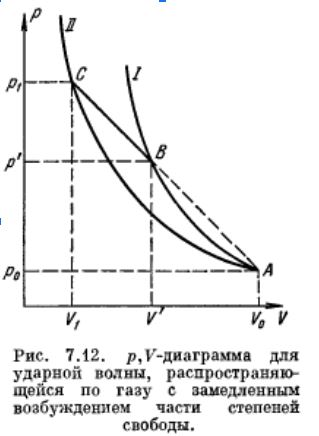
\includegraphics[width=50mm]{13. 2 udern adiab.JPG}}
	%\caption{\label{fig.2.4.1}}
	
	{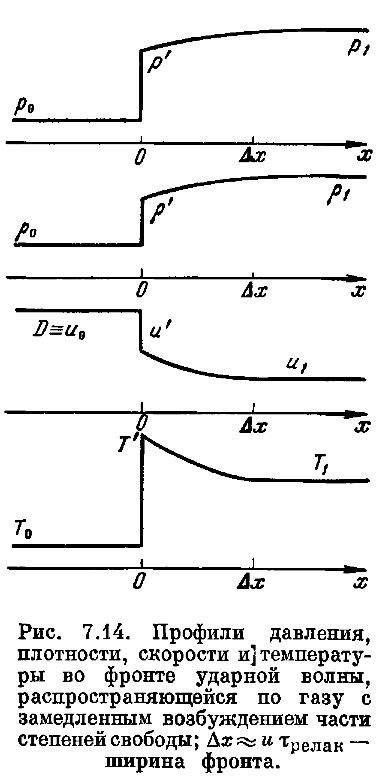
\includegraphics[width=50mm]{13.rel sloy.JPG}}
	%\caption{\label{fig.2.4.1}}
	
\end{figure}
В данном случае, у нас есть 2 адиабаты. Адиабата / проходит круче, чем II, как показано на рис. 7.12. Действительно, при одинаковой плотности температура и давление газа при 
условии замороженности некоторых степеней свободы выше, так как, грубо говоря, одинаковая энергия сжатия распределяется по меньшему числу степеней свободы.
В случае, если волна настолько слаба, что скорость ее меньше скорости звука, соответствующей замороженности части степеней свободы, прямая АС проходит ниже касательной к адиабате / в точке А (рис. 7.13). При этом состояние непрерывным образом, меняется вдоль прямой АС от точки А до точки С, и в газе с самого начала происходит постепенное возбуждение замедленной части теплоемкости. 

Поскольку в релаксационной зоне удельная энтальпия почти неизменна, а теплоемкость по мере возбуждения ранее замороженных степеней свободы возрастает, температура в ней уменьшается. Уменьшение температуры может быть довольно значительным, если запаздывающая часть теплоемкости велика и вносит большой вклад в конечную теплоёмкость газа. Конечная температура $Т_1$ может быть в два-три раза меньше температуры Т' за скачком уплотнения. Точно так же значительно может возрастать и плотность газа (грубо говоря, $р \sim \rho T$; р меняется мало, а Т сильно). Профили р, q, и, Т во фронте ударной волны, распространяющейся по газу с замедленным возвозбуждением части теплоемкости, изображены схематически на рис. ниже. 




\section{Прикладные проблемы физики плазмы}
\label{sec.14}


\subsection{Управляемый термоядерный синтез}
\label{14}

дейтерий + тритий = альфа-частица + нейтрон + 17.6 МэВ

[Кенро Миямото, Основы Физики Плазмы и управляемого термоядерного синтеза, Москва, физматлит 2007]

Всем известно про дефект масс, что при слиянии ядер до Fe и Ni выделяется энергия.
основная реакция D+T-> 4He + n [17.59 MeV], 1/5 энергии приходится на He и 4/5 на n
Чтобы сблизить ядра на достаточное расстояние надо преодолеть кулоновский барьер. ту силу, с которой они отталкиваются ($Z_{alpha}Z_p e^2/r_N$) вычислили, что примерное расстояние $r_{n}=1.4*10^{-13}*(A^{1/3}_{\alpha}+A^{1/3}_{\beta}) [cm]$ Но это оказалось слишком мало, ибо не сходилось с вычислениями T солнца, для 10кэВ вычислили точку остановки $R_t=10^{-11} [cm]$

[Миямото стр. 23]

Почему вообще надо удерживать плазму, какие характерные времена? Критерий Лоунсена 
Дело обстоит в том, что система должна сама себя поддерживать и при этом отдавать эл. энергию. Энергия в единице объёма $(3/2)nk(T_i+T_e)$. Время остывания $\tau_E = \frac { (3/2)nk(T_i+T_e) }{P_L+R}$, , где $P_L$ и $R$ соответственно мощность потерь энергии на диффузию и излучение плазмой. В то же время, в объёме происходит выделение тепла за счёт термоядерного синтеза мощностью. $P_{NF}=(n/2)(n/2)<\sigma v> Q_{NF} $. Потому
 как D и T присутствуют в реакторе в равном количестве и концентрация каждого n/2 соответственно. $<\sigma v> $ - вероятность процесса,   $Q_{NF} $ энергия на одну реакцию.
Чтобы всё было устойчиво и не затухало: $P_{heat}=P_L + R = \frac{3nkT}{\tau_E} < \eta_{el} \eta_{heat} P_{NF} $, где $\eta_{el} $ - КПД получения эл. мощности ,$ \eta_{heat} $ - КПД нагрева.

Итого: $ \frac{3nkT}{\tau_E} < \eta_{el} \eta_{heat} Q_{NF} n^{2} \frac{<\sigma v>}{4}$

\begin{equation}
	\label{eq.Disp14.1.1}
	n \tau_E > \frac{12 kT}{\eta Q_{NF} <\sigma v>} > 1.7*10^{20} m^{-3} s
\end{equation}
 - Критерий Лоунсена , критерий термоядерности. То есть надо или увеличивать концентрацию, или время удержания. Поэтому есть как токамаки с непрерывным временем работы, так и импульсные(импульсно поддерживается магнитное поле).
Понятно, что чем горячее плазма, тем труднее её удерживать, понятно что удерживать надо именно магнитным полем.

\subsection{Магнитное удержание}
\label{14.1}

Уравнения магнитной гидродинамики тут написаны [Голант Жилинский Сахаров, Основы ФП,  §10.1]

Из уравнения для средней скорости $\rho (du/dt)=(1/c)[j H]-grad\;p$; где $p=p_e+p_i$ - суммарное давление, $j=en(u_i+u_e)$ - плотность тока, $ du/dt=\delta u / \delta t + (u grad)u$ полная производная

можно вывести условие равновесия
\begin{equation}
	\label{eq.Disp14.1.2}
	\frac{1}{c}[j H]=grad\;p
\end{equation}
[Голант Жилинский Сахаров, Основы ФП,  §10.2]


Идея состоит в том, что преодолеть давление плазмы как газа с ооочень большой температурой с помощью давления магнитного поля около стенок.
Первая задача, возникающая при рассмотрении удержания плазмы в магнитном поле, заключается в определении условий, при которых достигается равновесие, т. е. электродинамические силы, действующие на каждый элемент объема плазмы, уравновешивают градиент давления.
\begin{equation}
	\label{eq.Disp14.1.3}
	G_H=\frac{1}{c} [j H]=\frac{1}{4 \pi} [H rotH]=-\frac{1}{8 \pi} grad(H^{2})+\frac{1}{4 \pi} (H grad) H
\end{equation}
Так же есть отдельный случай, когда линии имеют радиус кривизны R.

\begin{equation}
	\label{eq.Disp14.1.4}
(\vec H grad)\vec H=H(\vec h grad)\vec h H=H^{2} grad_{||}\vec h + \frac{1}{2} grad_{||} H^{2}=-H^{2} \frac{\vec R}{R}+\frac{1}{2} grad_{||} H^{2}
\end{equation}


, где $\vec h= \frac{\vec H}{H}$; $grad_{||}=(\vec h \; grad)$ - проекция градиента на направление магнитного поля. Подставляем в предыдущее выражение и получаем, что давление:
\begin{equation}
	\label{eq.Disp14.1.5}
 G_H=-grad_{\perp}(H^{2}/8\pi)-(H^{2}/4\pi R^{2})\vec R
\end{equation}
Первое слагаемое в представляет собой поперечный градиент введённого магнитного давления. Действие этой силы можно описать как взаимное «расталкивание» силовых линий в поперечном направлении. Второе слагаемое определяет силу, направленную к центру кривизны силовых линий, и называется натяжением магнитного поля. Оно формально получается, если приписать силовым линиям свойства растянутой струны.

Для равновесия: 
\begin{equation}
	\label{eq.Disp14.1.6}
 grad p + grad_{\perp}(H^{2}/8\pi)+(H^{2}/4\pi R^{2})\vec R =0
\end{equation}

Для случая, когда силовые линии прямые ($R\rightarrow \inf $), уравнение сводится к постоянству суммы кинетического и магнитного давлений в плоскости, перпендикулярной магнитному полю:
\begin{equation}
	\label{eq.Disp14.1.7}
p + H^{2}/8\pi=const
\end{equation}
\begin{equation}
	\label{eq.Disp14.1.8}
p_0 + H_{0}^{2}/8\pi=H_{e}^{2}/8\pi
\end{equation}

Равенство показывает, что максимальное давление плазмы, которое можно удерживать магнитным полем, равно магнитному давлению вне плазмы $H_{e}^{2}/8\pi$. При описании магнитного удержания часто вводят коэффициент $\beta$, представляющий собой
отношение давления удерживаемой плазмы к максимально возможному: $\beta=p/p_{max}=8\pi p/H_{e}^{2}$
Но это удержание поперёк линий магнитного поля, а строить комплексы в виде торов не всегда удобно, поэтому было придумано пробочное удержание.

пробочное удержание [Миямото стр. 32]

Понятно, что всё движение электрона в магнитном поле можно описать как движение вдоль и поперёк поля. Вдоль - свободное движение, поперёк - ларморовское вращение.
Если рассмотрим электрон в поле, он будет вращаться по кругу с радиусом равному Ларморовскому. Его можно представить в виде витка с током. У витка с током есть магнитный момент.
\begin{equation}
	\label{eq.Disp14.1.9}
 \mu=I*S=\frac{q\Omega}{2\pi} * \pi \frac{\rho^{2}}{2}=\frac{mv_{perp}^{2}}{2B}
\end{equation}	
Но кин энергия должна сохранятся при движении в магнитном поле, поэтому электрон будет лететь вдоль поля пока
\begin{equation}
	\label{eq.Disp14.1.10}
	\frac{mv_{||}^{2}}{2}+\frac{mv_{\perp}^{2}}{2}=\frac{mv^{2}}{2}=const
\end{equation}	
Поскольку магнитный момент сохраняется, то:
\begin{equation}
	\label{eq.Disp14.1.11}
 v_{||}=+-(\frac{2}{m}E-v_{\perp}^{2})^{1/2}=+-(v^{2}-\frac{2}{m} \mu B)^{1/2}
\end{equation}	
То есть электрон может полностью убрать продольную скорость и отразиться. Почему возникает этот эффект ? Потому что на магнитный диполь действует сила $-\mu \grad_{||}$ B. Ну и вводится пробочное отношение - отношение магнитных полей в центре и на краях ловушки $R_M=\frac{B_M}{B_0}$


\subsection{Плазменные источники излучения}
\label{14.4} 
раздел физики плазмы, изучающий коллективные взаимодействия плотных потоков (пучков), приводящие к возбуждению в системе линейных и нелинейных волн и колебаний, и использование эффектов такого взаимодействия.
плазменные ускорители, основанные на явлении коллективного ускорения тяжёлых частиц электронными пучками и волнами в плазме

плазменно-пучковый разряд, основанный на коллективном механизме взаимодействия плотных пучков заряженных частиц с газом;

турбулентный нагрев плазмы плотными пучками аряженных частиц и коллективных процессов при транспортировке и фокусировке пучков в проблеме управляемого термоядерного синтеза (УТС)

[Богданкевич Л С, Кузелев М В, Рухадзе А А "Плазменная СВЧ электроника" УФН 133 3–32 (1981)]
DOI: 10.3367/UFNr.0133.198101a.0003
URL: https://ufn.ru/ru/articles/1981/1/a/

Когда говорят о сильноточных электронных пучках, то прежде всего имеют в виду пучки с током, превышающим так называемый предельный вакуумный ток. Известно, что в металлическом волноводе с радиусом R и длиной $L >> R$, который обычно используется в вакуумной электронике в качестве резонатора, ток пучка ограничен пространственным зарядом электронов, причем предельный ток по порядку величины определяется соотношением:
\begin{equation}
	\omega_{b \; vol}^{2} \approx \frac{c^{2}}{S} \gamma
\end{equation}
, где $\gamma = [1-(u^{2}/c^{2})]^{-1/2}$ - — релятивистский фактор энергии электронов, $S$ — поперечное сечение пучка, меньшее или порядка сечения волновода, а $\omega_{b}=\sqrt{4\pi e^{2} n_{b} /m}$ — лэнгмюровская частота электронов пучка. 


Следовательно, сильноточным следует считать пучок, в котором $\omega_{b}^{2}>\omega_{b\;vol}^{2}$. Такой пучок может распространяться в волноводе только при наличии нейтрализации пространственного заряда электронов, что достигается заполнением системы относительно плотной (по сравнению с плотностью пучка) плазмой. Таким образом, сильноточная СВЧ электроника, строго говоря, может быть только плазменной. При этом, однако, плазма может и не влиять существенным образом на частоты генерируемых пучком электромагнитных волн. Дело в том, что длины волн возбуждаемых пучком электромагнитных колебаний меньше или порядка поперечных размеров электродинамической системы генератора, т. е. резонатора, точнее $\omega>\omega_{crit}= \mu c/R$, где $\mu$ характеризует радиальное волновое число моды колебаний (корни функций Бесселя или ее производных); обычно $\mu \sim 3-10$. Если плазма, заполняющая резонатор, имеет относительно низкую плотность, так что $\omega_{pl}=\sqrt{4\pi e^{2} n_{p} /m} < \mu c/R$ , то она существенно не меняет электродинамику резонатора, который по своим электродинамическим свойствам остается практически вакуумным. Вместе с тем такая плазма может нейтрализовать пространственный заряд пучка и позволить пропустить через резонатор сильноточный пучок со сверхпредельным током. Однако ток пучка при этом ненамного может превышать предельный, не более, чем в $\mu^{2} S/\gamma R^{2}$ раз, что следует из неравенств $\omega_{b}^{2}<\omega_{p}^{2}<\mu^{2} c^{2}/R^{2}$.

Иное положение имеет место в случае достаточно плотной плазмы, когда $\omega_{pl}>\mu c/R$. Роль такой плазмы в резонаторе не ограничивается нейтрализацией пространственного заряда пучка, она существенно меняет всю электродинамику резонатора и, в частности, спектры частот собственных электромагнитных мод резонатора. Именно в этом случае мы имеем дело с настоящей плазменной электроникой, которая, как будет видно из дальнейшего, позволяет продвинуться в область токов электронного пучка, намного превосходящих предельный вакуумный ток, вплоть до $\mu^{2}\gamma S/R^{2}$ раз. Более того, с помощью ультрарелятивистских электронных пучков в таких системах оказывается возможным эффективное возбуждение колебаний с длиной волны, намного меньшей поперечных размеров резонатора $\lambda \approx R/\gamma^{2}$ .

\begin{figure}[h!]
	\center{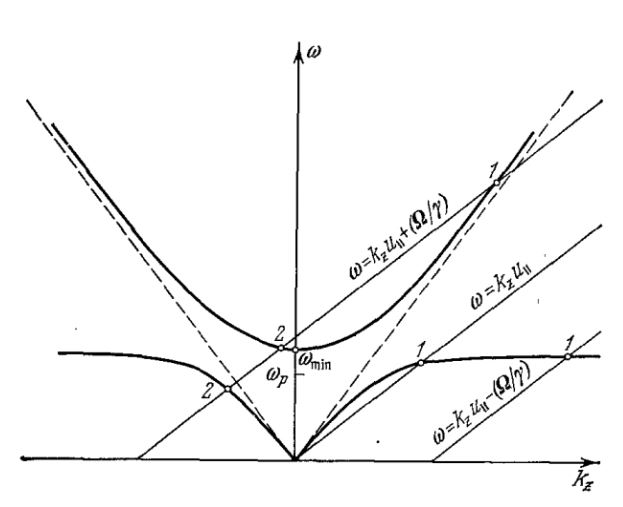
\includegraphics[width=70mm]{dispers_14_3.JPG}}
	%\caption{\label{fig.2.4.1}}
\end{figure}

Другими словами, плазменная СВЧ электроника открывает возможиость создания коротковолновых источников мощного электромагнитного излучения.


Без формул, наверное сразу можно нарисовать дисперсионку резонатора, без пучка.  Как мы видим при добвалении плазмы, появилась ещё одна нижняя ветвь. Точки 1. это работа в режиме усилителя. Пучок (наклонные линии $\omega=ku\pm (\Omega/\gamma)$) усиливает волну бегущую в ту же сторону. Точки 2. это работа в режиме генератора. Пучок усиливает встречную волну.



плазменная СВЧ электроника.
Компрессоры импульсов.


\subsection{Преобразование тепловой энергии в электрическую: МГД-преобразователи, тепловые преобразователи}
\label{14.5} 
[райзер, дополнение, стр. 673]

\begin{figure}[h!]
	\center{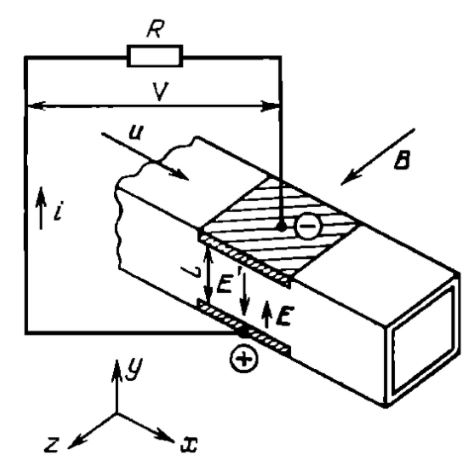
\includegraphics[width=70mm]{MGD_generator.JPG}}
	%\caption{\label{fig.2.4.1}}
\end{figure}

Принцип работы МГД генератора представлен на рисунке. Ионизованный газ протекает по каналу со скоростью и и пересекает линии напряженности приложенного постоянного магнитного поля. В движущейся среде индуцируется электрическое поле $Е' =\frac{1}{c} [V\; В]$. Вектор магнитной индукции $В =\mu H$ не отличается от $Н$, поскольку магнитная проницаемость газа $\mu=1$. Направление Е' характеризуется  
координатным равенством $E’_y=-u_x B_z / c $. Индуцированное поле Е' движет электроны вверх. У верхней  
стенки канала накапливается отрицательный пространственный заряд, у нижней — положительный. Если внешняя цепь между электродами, помещенными на этих стенках, разомкнута, заряды накапливаются, пока созданное ими электрическое поле $E_{\inf}$ не уничтожит индуцированное ($E_{\inf}=-E’$). Потенциал нижнего электрода при этом превышает потенциал верхнего на $V_{\inf} = E_{inf} L$. Это напряжение совпадает по величине с ЭДС генератора:
\begin{equation}
	\varepsilon=E’_{y}L=(-u_x /c)(B_z L)
\end{equation}

Если цепь замкнуть через нагрузочное сопротивление и обеспечить достаточно высокую электронную эмиссию с нижнего электрода, например путем его активирования и нагревания, в цепи потечет ток. Реально электроны в газе непрерывным потоком дрейфуют вверх, исходя из нижнего положительного электрода, который в отличие от обычного разряда работает подобно катоду, и внедряясь в верхний. Частичное устранение приэлектродного пространственного заряда, уносимого током, приводит к уменьшению напряжения на электродах $V= Е_{y} L$ по сравнению с $V_{inf}=|\varepsilon|$. В пренебрежении эффектом Холла, в результате которого возникает ток по оси $х \perp Е, В$, плотность тока в газе:
\begin{equation}
	j=\sigma(E+E’)=\sigma(E+\frac{1}{c}[u\;B])
\end{equation}

Ну или в нашей системе координат 
\begin{equation}
	j_y=\sigma(E_y-\frac{[u\;B]}{c}) <0
\end{equation}

Дело ещё обстоит в том, что ток в цепи как раз и зависит от E меж электрожного промежутка, как $i*R=V$ (общий ток через систему с площадью $S$, $i=j*S$), в то время как $V=E*L$, то есть мы получили систему самосогласованных уравнений, которые замкнулись сами на себя. А именно:
\begin{equation}
	i=S \sigma(V/L-uB/c)=S \sigma(iR/L-uB/c)
\end{equation}
отсюда можно выразить $i$ в чистом виде. $i=\frac{u\;B}{c(\frac{R}{L}-\frac{1}{\sigma S})}$

При протекании тока на газ действует тормозящая пондеромоторная сила, в результате чего он и теряет энергию. Отношение мощности, выделяемой в нагрузке, к мощности, отбираемой от газа: 
\begin{equation}
	\frac{iV}{(u/c)(jB)LS}=\frac{V}{\varepsilon}
\end{equation}

т. е. электрический КПД генератора тем выше, чем ближе ситуация к режиму разомкнутой цепи. Но абсолютное значение полезной мощности $iV$ максимально, когда сопротивления нагрузки и плазмы одинаковы и $V=|\varepsilon|/2$


\subsection{Химические реакции в равновесной и неравновесной плазме. \textcolor[rgb]{1,0,0}{Механизмы и кинетика осуществления плазмохимических реакций, роль заряженных и возбужденных частиц. Энергетика химических реакций в электрических разрядах}. Закалка продуктов плазмохимических процессов.}

\label{14.6}

 
[В.Д. Русанов, А.А. Фридман, Физика химически-активной плазмы]

Очевидно, что хотели увеличить скорость некоторых процессов и сократить их количество. Поэтому некоторые реакции хотели провести напрямую в плазме. В рамках классической кинетики при этом экспоненциально ускоряется в соответствии с известным законом Аррениуса $ к \sim exp(-E_{a}/T)$, где $E_a$ — характерная величина энергетического барьера реакции; Т — температура системы. (Понятно, что хим реакция протекает при столкновении двух/трёх частиц, каждая из которых может быть подчинена максвеллу).
 
Резкое повышение скорости процесса может иметь место уже при температурах 3000—5000° С, что значительно выше обычного диапазона температур химических, технологических и  металлургических процессов. Скорость переноса реагентов через зону реакции, очевидно, должна соответствовать повышенной удельной производительности, которая достигается в реакционной зоне при очень высоких температурах, что можно реализовать только в случае газового транспорта реагентов с повышенными скоростями ($5*10^{3}—5*10^{4}$ см/с). 
Очевидно, что подвод к газу столь высокопотенциального тепла не может быть осуществлен с помощью традиционных методов теплопередачи. Сверхвысокие температуры в реакционной зоне должны обеспечиваться подводом энергии электромагнитного поля от внешнего источника, а не тепловой энергии. Этим требованиям отвечает совмещение реакционной зоны с газоразрядной, в которой можно организовать локальный нагрев реагентов до высоких температур за счет активных потерь энергии электромагнитного поля.

Плазмохимические системы в целом можно условно разделить на два больших класса — квазиравновесные и неравновесные.
Температура Т в случае, когда система близка к равновесию (квазиравновесию), является единственной энергетической характеристикой системы, т. е. $Т \approx T_{o} \approx Т_{e} \approx T_{i} \approx  Т_{r} = T_{v}$, где $Т_{o}$ — поступательная температура нейтрального газа, $Т_e$ — температура электронов; $Т_i$ — температура ионов; $Т_r$ — вращательная температура молекул; $T_v$— колебательная температура молекулярного газа. 

Если равновесие в системе не достигнуто, то могут реализоваться различные неравновесные (неизотермические) ситуации, из которых наибольший практический интерес с точки зрения оптимизации характеристик реакционной зоны имеют простейшие системы 

\begin{equation}
T_e \textgreater T_0, T_i, T_v,T_r
\end{equation}

\begin{equation}
T_e \textgreater T_i \textgreater T_0  \approx T_v  \approx T_r
\end{equation}

Неравновесность первого типа представляется наиболее универсальной, при этом концентрация электронов в реакционной зоне оказывается существенно ниже, чем определенная формулой Саха по температуре электронов Те, но на много порядков больше величины пе, определенной по этой же формуле для температуры  нейтральных частиц $Т_0$. Частный случай неравновесной системы, реализуемой во втором случае, связан не только с отрывом температуры электронов, но также с отрывом колебательной температуры  молекул от вращательной и поступательной температуры газа, который может обеспечить реализацию химических процессов через колебательное возбуждение реагирующих молекул. 

При накачке электронным ударом происходит преимущественное заселение нижних колебательных уровней молекул. Заселение высоковозбужденных состояний, проявляющих химическую активность, происходит в основном за счет обмена колебательными квантами. В результате этого процесса с учетом ангармонизма молекул могут возникать распределения по колебательным состояниям, заметно отличающиеся от больцмановского $f(v) \sim ехр(-\hbar \omega \nu / T_v)$, где $\hbar \omega \nu$ - колебательная энергия. Например, для простейшего случая двухатомных молекул учет ангармонизма ($х_e$) приводит к обогащению заселенности высоковозбужденных состояний согласно соотношению Тринора:

\begin{equation}
  f(v) \sim ехр(-\frac{\hbar \omega \nu} {T_v}+x_e\frac{\hbar \omega \nu^{2}}{T_0})
\end{equation}

Доля высоковозбужденных реакционноспособных молекул согласно этому соотношению может быть выше больцмановской на много порядков. Соответственно высокими оказываются и скорости плазмохимических процессов. Это позволяет подавить вредное влияние релаксации и обратных химических реакций, обеспечивая в итоге высокую энергетическую эффективность. 

Подробнее остановимся на неравновесных разрядах. [Д.И. Словецкий, механизмы химических реакций в неравновесной плазме]
Именно на практике термин чаще встречается “неравновесный разряд” в отношении возбуждённых частиц. А именно это распространено в создании мощных газоразрядных лазеров. Понятно, что нам энергетически выгодно заселять только тот уровень, который бы потом излучил. С ростом энергии у нас будут сначала будет возбуждаться поступательная степень свободы, потом вращательная и самая последняя - колебательная. И вот иногда, во время столкновений нейтрала с возбуждённой частицей может возбудиться именно колебательная степень свободы, минуя первые две. тем самым, у нас создаётся неравновесное распределение заселённости по уровням.
В таком случае, вообще, надо начинать заного писать кин уравнение для частиц сорта A на уровне i.
\begin{equation}
\frac{\delta [A(i)] f_{A(i)}}{\delta t}+\frac{F_A}{M_A}\frac{\delta [A(i)] f_{A(i)}}{\delta V_A} +v_A \frac{\delta [A(i)] f_{A(i)}}{\delta r}=\sum_{S,n} I(A,i|S,n) 
\end{equation}

Поскольку классическая химическая кинетика имела дело с сумарными концентрациями чатиц определённого сорта, то и в этом случае можно просуммировать концентрации по всем уровням энергии интегрируя по всем скоростям можно получить
 \begin{equation}
-\frac{d [A] }{dt}=k(C,D|A,B) [A][B]-k(A,B|C,D) [C][D]
\end{equation}
В общем случае коэффициенты реакции могут зависеть от всего на свете, они так же могут иметь пороговый характер. И для описания неравновесных процессов обычно выписываются все уравнения для основных уровней всех веществ, участвующих в реакции и решается на компьютере.

[Неравновесная колебательная кинетика, под редакцией М. Капителли, пункт 4, стр 105]

Самые основные процессы в такой плазме $VT$ (колебательно поступательный), $VV$ (колебательно колебательный) обмен энергии. (много непонятной теории)

\subsection{Методы диагностики химически активной плазмы.}
\label{14.7} 


 [словецкий, стр 39]

\subsection{Взаимодействие плазмы с поверхностью твердых тел. Плазменные технологии (травление, имплантация, упрочнение, нанесение покрытий и пр.)}
\label{14.8}


 [СТЕПАНОВСКИЙ А. С. ИОННАЯ ОБРАБОТКА МАТЕРИАЛОВ ]


В зависимости от параметров ионного или электронного потока в поверхностном слое деталей могут происходить различные процессы. При энергии ионов (уже не инертного газа) $E \approx 10…100 эВ$ на поверхности детали происходит конденсация ионов. Такая обработка используется для осаждения покрытий. Если $E \approx 10^2…10^3 эВ$, то реализуется процесс ионного распыления (травления), который применяется для очистки поверхностей деталей, активирования поверхностного слоя, формирования микрорельефа. При $E > 10^4 эВ$ происходит ионная имплантация, т.е. внедрение ионов имплантируемого вещества в поверхностный слой детали. Таким образом, можно модифицировать поверхностный слой путем его легирования практически любыми элементами. Имплантация приводит к увеличению концентрации дефектов в облучаемом материале, которые в этом случае называют радиационным. При больших дозах облучения поверхностного слоя детали становятся аморфными из-за высокой концентрации радиационных дефектов. Ионная бомбардировка и облучение электронами приводит к нагреву поверхностного слоя, а в ряде случаев наблюдается образование газовых пузырьков и микропор, которые приводят к уменьшению плотности материала


При плазменном травлении обрабатываемый образец помещается непосредственно в область химически активной плазмы, располагаясь на специальном подложкодержателе, и
находится обычно под плавающим потенциалом. Основными частицами, участвующими в процессе плазменного травления и влияющими на него, являются свободные атомы, радикалы, ионы и электроны. Вклад этих частиц в плазменное травление различен: химически активные частицы, т.е. свободные атомы и радикалы, вступают в химическую реакцию с поверхностными атомами материалов и удаляют поверхностные слои в
результате образования летучих продуктов реакции, а электроны и ионы активируют эту реакцию, увеличивая скорость травления. Активирующее воздействие ионов и электронов
определяется энергией, с которой они бомбардируют обрабатываемую поверхность. К плазменному травлению относятся процессы, в которых энергия ионов не превышает 100 эВ.

\title{Билеты к кандидатскому экзамену по физике плазмы: дополнительная программа}

\maketitle

\section{Кинетический и гидродинамический методы описания плазмы}

\subsection{Уравнение Лиувилля и условия корректного перехода к кинетическому уравнению с самосогласованным полем для одночастичной функции распределения. Разлет бесстолкновительной плазмы (ограниченной и из полупространства)}

Уравнение Лиувилля = уравнение Больцмана в бесстолкновительном приближении -- уравнение, описывающее изменение функции распределения (ФР) частиц плазмы определённого сорта.

Вывод уравнения Лиувилля можно посмотреть перед~\ref{eq:Liouville_eq}. Приведём здесь его ещё раз:

\begin{equation}
	\frac{df}{dt} = \frac{\partial f}{\partial t} + \frac{d\vec{r}}{dt}\frac{\partial f}{\partial \vec{r}}+ \frac{\vec{F}}{m}\frac{\partial f}{\partial \vec{v}} = 0
\end{equation}


\subsection[Приближенное описание столкновений в рамках кинетического уравнения. Интеграл столкновений в форме Ландау, уравнение Фоккера-Планка, релаксационная форма интеграла 	столкновений ($\tau$-приближение). Кинетическое описание упругих и неупругих столкновений электронов с атомами и молекулами. Приближенное описание кинетики электронов в слабом однородном электрическом поле (расчет эффективной частоты столкновений и нагрева электронов). Явление убегающих электронов]{Приближенное описание столкновений в рамках кинетического уравнения. Интеграл столкновений в форме Ландау, уравнение Фоккера-Планка, релаксационная форма интеграла 	столкновений \linebreak ($\tau$-приближение). Кинетическое описание упругих и неупругих столкновений электронов с атомами и молекулами. Приближенное описание кинетики электронов в слабом однородном электрическом поле (расчет эффективной частоты столкновений и нагрева электронов). Явление убегающих электронов} \label{subsec:collision_terms}

\subsubsection{Приближенное описание столкновений в рамках кинетического уравнения}

Столкновения в рамках кинетического уравнения описываются с помощью интеграла столкновений (см. формулу~\ref{eq:Boltzmann_eq}). В целом, больцмановский подход предполагает рассмотрение только парных столкновений и замыкание системы (см. выше приближение Больцмана~\ref{eq:Boltzmann_relation}). Считаем, что столкновения резко меняют скорости частиц и не нарушают их расположения в пространстве (точечность столкновений). Плазма -- локально однородна, слагаемое в кин. уравнении $\sim \frac{\partial}{\partial \vec{r}}$ можно рассматривать как снос. Изменение скоростей можно рассматривать в отдельности от изменения координат\Tokman.

Пусть выражение (\ref{eq:Liouville_eq}) записано для частиц сорта $\alpha$ и $\beta$. Будем учитывать в интеграла столкновений соударения между частицами как одного, так и двух разных сортов. Пусть $\Gamma_\alpha$ -- совокупность всех внутренних координат частиц сорта $\alpha$ [в т.ч. -- квантовых чисел = их распределение по уровням; пока мы не определили, упругие или неупругие взаимодействия -- общий случай]. Формально это учитывается в определении концентрации:

\begin{equation*}
	n(\vec{r}, t) = \int\limits_{\infty}f(\Gamma_\alpha,\vec{r},t)dv_\alpha,
\end{equation*}

где $\vec{r}$ -- относительно центра масс данной частицы.

Задача: определить число столкновений частиц определённого сорта в определённом интервале. Столкновения в ``реальном'' пространстве приводят к уходу частиц из одной области фазового ($\Gamma-$) пространства в другую. По сути, отношение числа частиц к объёму и есть ФР.

\begin{figure}[h!]
	\begin{center}
		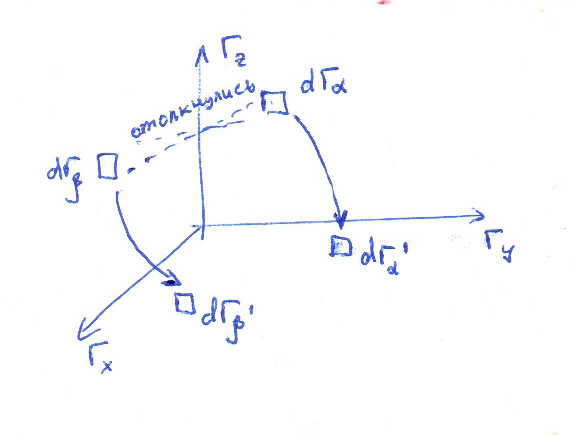
\includegraphics[width=0.45\linewidth]{boltzmann_collision_term.pdf}
	\end{center}
	\caption{Рисунок из лекций}
	\label{fig:boltzmann_collision_term}
\end{figure}

Пришло в объём $d\Gamma_\alpha$:

\begin{equation*}
	dQ_\alpha^{(+)} = d\Gamma_\alpha \int\limits_{\infty}d\Gamma_\alpha^{'} \int\limits_{\infty}d\Gamma_\beta^{'} \int\limits_{\infty}d\Gamma_\beta \cdot f_{\alpha\beta}\left(\Gamma_\alpha^{'} \Gamma_\beta^{'}\right) \cdot \omega_{\alpha\beta}\left(\Gamma_\alpha, \Gamma_\beta, \Gamma_\alpha^{'}, \Gamma_\beta^{'}\right)
\end{equation*}

Ушло из объёма $d\Gamma_\alpha$:

\begin{equation*}
	dQ_\alpha^{(-)} = d\Gamma_\alpha \int\limits_{\infty}d\Gamma_\alpha^{'} \int\limits_{\infty}d\Gamma_\beta^{'} \int\limits_{\infty}d\Gamma_\beta \cdot f_{\alpha\beta}\left(\Gamma_\alpha \Gamma_\beta\right) \cdot \omega_{\alpha\beta}\left(\Gamma_\alpha^{'}, \Gamma_\beta^{'}, \Gamma_\alpha, \Gamma_\beta\right),
\end{equation*}

где выбрано обозначение $\omega_{\alpha\beta}(A, B, C, D)=\omega_{\alpha\beta}(C\rightarrow A, D\rightarrow B)$.

Важно: $\omega(\ldots)\neq 0$ -- только для работающих законов сохранения (в выражении) -- 

\begin{equation*}
	\omega_{\alpha\beta} = \omega\left(\Gamma_\alpha, \Gamma_\beta, \Gamma_\alpha^{'}, \Gamma_\beta^{'}\right)\cdot\delta(\text{ЗСЭ}) \delta(\text{ЗСИ})\delta(\ldots) \sigma_{\alpha\beta}\abs{\overrightarrow{v_\alpha}-\overrightarrow{v_\beta}}
\end{equation*}

Последняя дельта-функция иллюстрирует собой особенности конкретного процесса (например, учёт упругости столкновения).

Тогда столкновительный интеграл (изменение ФР под воздействием столкновений):

\begin{equation*}
	St = \frac{dQ_\alpha^{(+)}-dQ_\alpha^{(-)}}{d\Gamma_\alpha}
\end{equation*}

\begin{equation*}
	St_\alpha = \int\limits_{\infty}d\Gamma_\alpha^{'} \int\limits_{\infty}d\Gamma_\beta^{'} \int\limits_{\infty}d\Gamma_\beta \cdot \omega_{\alpha\beta}\left(\Gamma_\alpha, \Gamma_\beta, \Gamma_\alpha^{'}, \Gamma_\beta^{'}\right) \cdot (f_{\alpha\beta}^{'}-f_{\alpha\beta}) \xrightarrow{\text{малое взаимодействие}}
\end{equation*}

Интеграл соударений в форме Больцмана:

\begin{equation} \label{eq:Boltzmann_collision_term}
	\rightarrow \int\limits_{\infty}d\Gamma_\alpha^{'} \int\limits_{\infty}d\Gamma_\beta^{'} \int\limits_{\infty}d\Gamma_\beta \cdot \omega_{\alpha\beta}\left(\Gamma_\alpha, \Gamma_\beta, \Gamma_\alpha^{'}, \Gamma_\beta^{'}\right) \cdot (f_{\alpha}^{'}f_{\beta}^{'}-f_{\alpha}f_{\beta})
\end{equation}

Случай упругих столкновений: $d\Gamma_{\alpha, \beta}\rightarrow v_{\alpha, \beta}$. В случае неупругих имеет место, например, переход между различными состояниями частиц одного и того же сорта или др. Кроме того, если есть динамические изменения внутренних степеней свободы под действием полей, то надо либо слева в уравнение~(\ref{eq:Boltzmann_eq}) дописать $\dot{\Gamma}_{\text{прочие}}\frac{\partial f_\alpha}{\partial \Gamma_{\text{прочие}}}$, либо справа поменять интеграл столкновений на выражение $\int\limits_{\infty}d\Gamma_{\text{прочие}}St_{\alpha\beta}\left\lbrace f_\alpha\right\rbrace$.

Важно: если у нас было 2 максвелловских распределения, с одинаковой температурой, то и после столкновений будут те же распределения с точно такой же температурой. 

Важно: Больцмановская форма интеграла столкновений основана на предположении, которое в общем случае несправедливо для полностью ионизованной плазмы: длительность столкновения много меньше времени между столкновениями. В плазме длительность столкновения совпадает со временем пролета частицей длины, равной дебаевскому радиусу экранирования. Этот интервал времени значительно превышает интервал времени между столкновениями, поскольку электрон, например, входит в дебаевскую сферу следующего иона задолго до того, как он покидает дебаевскую сферу предыдущего иона. Таким образом, в течение времени столкновения взаимодействие отнюдь не парное: электрон одновременно взаимодействует со всеми остальными частицами в дебаевской сфере, число которых велико согласно предположению.

Для того чтобы правильно учесть столкновения в плазме, необходимо построить более подходящую модель для интеграла столкновений. Пример: уравнение Фоккера-Планка.

\subsubsection{Интеграл столкновений в форме Ландау, уравнение Фоккера-Планка}

Рассмотрим набор переменных $\Gamma_\alpha$ -- только скорости. Тогда

\begin{equation*}
	\frac{df}{dt} = St_{\alpha\beta}\left\lbrace f_\alpha\right\rbrace = \int\limits_{\infty}dv_\alpha^{'} \int\limits_{\infty}dv_\beta^{'} \int\limits_{\infty}dv_\beta \cdot \omega_{\alpha\beta}\left(v_\alpha, v_\beta, v_\alpha^{'}, v_\beta^{'}\right) \cdot (f_{\alpha}^{'}f_{\beta}^{'}-f_{\alpha}f_{\beta})
\end{equation*}

Рассмотрим случай неподвижной до и после частицы сорта $\beta$. Это соответствует случаю либо рассеянию электрона на ионе, либо рассеянию небольшой группы электронов на электронах всей функции распределения так, что она не меняется. Тогда:

\begin{equation*}
	\int\limits_{\infty} d^3v_\beta^{'}\left(f_\beta^{'}f_\alpha^{'}-f_\beta f_\alpha\right) = f_\beta\left(f_\alpha^{'}-f_\alpha\right)
\end{equation*}

\begin{equation*}
	\omega_{\alpha\beta}\left(v_\alpha, v_\beta, v_\alpha^{'}, v_\beta^{'}\right) \rightarrow \omega_{\alpha\beta}\left(v_\alpha, v_\beta, v_\alpha^{'}\right)
\end{equation*}

Пусть $\overrightarrow{v_\alpha^{'}}=\overrightarrow{v_\alpha}+\overrightarrow{\Delta v}$. Перейдём к интералу по ``перескоку'' $\Delta v$.

\begin{equation*}
	St_{\alpha\beta}\left\lbrace f_\alpha\right\rbrace = \int\limits_{\infty}d^3v_\beta f_\beta \int\limits_{\infty} d^3\Delta v \cdot \widetilde{\omega}(\overrightarrow{v_\beta}, \overrightarrow{v_\alpha}+\overrightarrow{\Delta v}, \overrightarrow{\Delta v}) \cdot \left(f_\alpha\left(\overrightarrow{v_\alpha}+\overrightarrow{\Delta v}\right)-f_\alpha\left(\overrightarrow{v_\alpha}\right)\right)
\end{equation*}

(введена $\widetilde{\omega}$ как переобозначение $\omega_{\alpha\beta}$). Зависит от точки ``прыжка'' ($\overrightarrow{v_\alpha}$) и длины ``перескока'' ($\Delta v$) [в фазовом пространстве]. Будем считать, что самая большая вероятность перескока связана с изменением на малую величину. Аналогия/физическая обоснованность предположения: броуновское движение, где средний перескок тоже мал. Раскладываем по $\overrightarrow{\Delta v}$ в ряд.

\begin{equation*}
	St_{\alpha\beta}\left\lbrace f_\alpha\right\rbrace \approx \int\limits_{\infty} d^3v_\beta f_\beta \int\limits_{\infty}d^3\Delta v \cdot \left( \widetilde{\omega}(\overrightarrow{v_\beta}, \overrightarrow{v_\alpha}, \overrightarrow{\Delta v})+\frac{\partial \widetilde{\omega}}{\partial \overrightarrow{v_\alpha}}\overrightarrow{\Delta v} \right) \cdot \left(\overrightarrow{\Delta v}\frac{\partial f_\alpha}{\partial \overrightarrow{v_\alpha}}+\sum\limits_{i}\frac{1}{2}\overrightarrow{\Delta v_i}^2\frac{\partial^2f_\alpha}{\partial \overrightarrow{v_{\alpha_{i}}}^2}\right)
\end{equation*}

Тогда возникает \uline{уравнение Фоккера-Планка}:

\begin{equation} \label{eq:Fokker-Planck_eq}
	\frac{df_\alpha}{dt} = St_{\alpha\beta}\left\lbrace f_\alpha\right\rbrace = \frac{\partial}{\partial \overrightarrow{v_\alpha}} \left(\vec{A}f_\alpha\right) + \sum\limits_{i,j}\frac{\partial^2}{\partial v_{\alpha_{j}}\partial v_{\alpha_{i}}} \left(B_{ji}f_\alpha\right),
\end{equation}

где \uline{коэффициенты Эйнштейна} $\vec{A}$ и $B_{ji}$ равны соответственно:

\begin{equation*}
	\vec{A} = \int\limits_{\infty} d^3v_\beta f_\beta \int\limits_{\infty} d^3\Delta v \cdot \overrightarrow{\Delta v} \cdot \widetilde{\omega} (\overrightarrow{v_\beta}, \overrightarrow{v_\alpha}, \overrightarrow{\Delta v})
\end{equation*}

\begin{equation*}
	B_{ji} = \frac{1}{2} \int\limits_{\infty} d^3v_\beta f_\beta \int\limits_{\infty} d^3\Delta v \cdot \Delta v_j \Delta v_i \cdot \widetilde{\omega} (\overrightarrow{v_\beta}, \overrightarrow{v_\alpha}, \overrightarrow{\Delta v})
\end{equation*}

Иногда используют следующую запись:

\begin{equation*}
	St_{\alpha\beta}\left\lbrace f_\alpha\right\rbrace = div_{\vec{v}} \left(\vec{A}f_\alpha+\frac{\partial \vec{B_j}f_\alpha}{\partial v_j}\right) = -div_{\vec{v}}\Gamma_v,
\end{equation*}

откуда кинетическое уравнение может быть записано в форме:

\begin{equation*}
	\frac{\partial f_\alpha}{\partial t}+\vec{v}\frac{\partial f_\alpha}{\partial \vec{r}}+\frac{\partial}{\partial \vec{v}}\left(\frac{\vec{F}}{m}f_\alpha+\Gamma_v\right)
\end{equation*}

Для кулоновских соударений \uline{Ландау} приводит явный \uline{вид интеграла столкновений}\Tokman:

\begin{equation} \label{eq:Landau_collision_term}
	\Gamma_{v_{k}} = \frac{1}{2}\mu_{\alpha\beta}\sum\limits_{l}\int d^3v_\beta \nu_{\alpha\beta}^t(v_{\alpha\beta}) (v^2\delta_{kl}-v_lv_k)\left\{f_\alpha\frac{\partial f_\beta}{\partial v_{\beta_{k}}}-\frac{m_\beta}{m_\alpha}f_\beta\frac{\partial f_\alpha}{\partial v_{\alpha_{k}}}\right\}
\end{equation}

Средняя скорость будет равна $<\vec{v_\alpha}> = -\int\limits_{\infty}d^3v_\alpha \vec{A}f_\alpha$, поэтому $\vec{A}$ и $B_{ji}$ соответствуют силе динамического трения [уменьшения скорости некоторой группы частиц; $\sim \frac{F_eff}{m}$] и диффузии [уширение распределения; $\sim D_{ji}(v)$ -- коэффициент диффузии] соответственно. 

При распределении частиц сортов $\alpha$ и $\beta$ по Максвеллу интеграл равен 0.

Существует связь коэффициентов $\vec{A}$ и $B_{ji}$ -- т.н. \uline{соотношения Эйнштейна}:

\begin{equation} \label{eq:Einstein_relation}
	\frac{T}{m_\alpha}A_j = \sum\limits_{i} B_{ji} v_{\alpha_{i}}
\end{equation}

Применяется для следующих случаев:

\begin{enumerate} 
	\item лёгкий газ в тяжелом
	\item кулоновское рассеяние (дальнодействующее)
	\item рассеяние малого числа частиц на равновесном распределённом объёме
\end{enumerate}


\subsubsection{Релаксационная форма интеграла 	столкновений \linebreak ($\tau$-приближение)}

\uline{Интеграл соударений в форме БГК [Бхатнагара–Гросса–Крука]} подробно введён в~\ref{subsec: maxwellization_time}. Напишем здесь лишь его вид:

\begin{equation} \label{eq:BGK_collision_term}
	\frac{df_\alpha}{dt} = St\left\lbrace f_\alpha\right\rbrace = \frac{f_0-f_\alpha}{\tau},
\end{equation}

т.е. $f_\alpha = f_0 + C\cdot exp(-t/\tau)$ -- т.н. $\tau$-приближение, где $\tau$ -- обратная транспортная частота/время максвеллизации/время релаксации.

Условие нормировки: $\int\limits_{\infty}f_\alpha d^3v =\int\limits_{\infty}f_0d^3v = n$.

\subsection{Моменты функции распределения и переход к гидродинамическому описанию плазмы. Приближение квазигидродинамики, вывод диффузионных уравнений, явление термодиффузии и теплопроводности. Амбиполярная диффузия. ``Вмороженность'' магнитного поля в плазму. Нагрев электронов в постоянном и высокочастотном электрическом поле при наличии столкновений}

Какой-то текст 3

\section{Движение заряженных частиц в электрическом и магнитном полях}

Какой-то текст 4

\subsection{Релятивистские уравнения движения заряженных частиц в электромагнитном поле. Точные решения в однородных постоянных полях и в поле бегущей плоской волны}

Какой-то текст 5

\subsection{Движение заряженной частицы в магнитной ловушке, адиабатические инварианты, неоклассический перенос}

Какой-то текст 6

\subsection{Движение частицы в слабо неоднородном высокочастотном электромагнитном поле, высокочастотный потенциал, влияние внешнего магнитного поля}

Какой-то текст 7

\subsection{Движение электрона в пространственно периодическом электрическом поле. Квазиимпульс и зонный спектр электронов. Экранировка зарядов в кристалле в приближении случайных фаз}

Какой-то текст 8

\section{Волны в плазме}

Какой-то текст 9

\subsection{Феноменологическое описание электродинамики сред с временной и пространственной дисперсией. Плоские монохроматические волны, тензор диэлектрической проницаемости, 	соотношение Крамерса-Кронига. Распространение волновых пакетов, плотность энергии и потока энергии квазимонохроматических электромагнитных волн в среде с временной дисперсией, волны с отрицательной энергией}

Какой-то текст 10

\subsection{Тензор диэлектрической проницаемости в холодной магнитоактивной плазме. Электромагнитные и потенциальные волны в изотропной плазме с учетом теплового движения в рамках гидродинамического описания. Классификация волн в магнитоактивной плазме. Тензор диэлектрической проницаемости плазмы в рамках кинетического описания}

Какой-то текст 11

\subsection{Распространение электромагнитных волн в плоско-слоистой плазме. Нормальный и аномальный скин-эффект. Поглощение волн в областях плазменного и циклотронного резонанса. Линейная трансформация волн в изотропной плазме и магнитоактивной плазме, эффект предельной поляризации волн}

Какой-то текст 12

\subsection{Поверхностные волны на границе плазменного полупространства. Каналирование волн в плоских слоях с повышенной и пониженной плотностью плазмы. Резонансные характеристики простейших плазменных объектов – плоский слой, цилиндр, шар}

Какой-то текст 13

\subsection{Геометрооптическое описание волн в нестационарной плоскослоистой изотропной плазме. Геометрическая оптика в магнитоактивной плазме}

Какой-то текст 14

\section{Взаимодействие заряженных частиц с волнами в плазме}

Какой-то текст 15

\subsection{Понятие об абсолютной и конвективной неустойчивости. Кинетические и гидродинамические неустойчивости электромагнитных волн в плазме (примеры)}

Какой-то текст 16

\subsection{Эволюция функции распределения электронов в поле монохроматической плазменной волны. Квазилинейная теория, релаксация электронного пучка в плазме, ускорение частиц 	плазменной турбулентностью, механизм Ферми, формирование энергетического спектра частиц}
\subsubsection{Эволюция функции распределения электронов в поле монохроматической плазменной волны}
[Кадомцев, 2-е изд. стр. 186]
Пусть у нас летит плоская волна в плазме с какой-то функцией распределения. Введём их координату $\xi$ как отклонение от фронта волны с координатой “х”.
Уравнение тогда будет:
\begin{equation}
	\frac{d^2}{dt^{2}} \xi (x,t) = - \frac{e}{m_e} E(x+\xi,t)
\end{equation}
Эл поле определяется $E(x+\xi,t)=4 \pi e n_0 \xi$, тогда уравнение примет вид:
\begin{equation}
	\frac{d^2}{dt^{2}} \xi = - \omega^{2}_{pe} \xi
\end{equation}
\begin{figure}[h!]
	\center{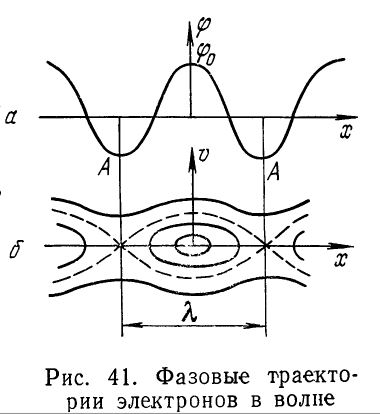
\includegraphics[width=70mm]{zatuh_landau_nonlinear_1.JPG}}
	%\caption{\label{fig.2.4.1}}
\end{figure}
То есть, видно, что электроны могут осциллировать в поле волны, которая летит через плазму. То есть в приближении холодной плазмы можно считать, что ленгмюровская волна имеет малую, но конечную амплитуду и её потенциал является гармонической функцией вида $\phi = \phi_0 cos(\omega_{pe} t -kx)$ .  Из-за теплового разброса будет происходить взаимодействие с резонансными частицами в плазме. Посмотрим, как будет двигаться электрон в таком потенциале. Перейдём в с.о. связанную с волной. Потенциал будет иметь вид $\phi = \phi_0 cos(kx)$. Ф.П. - кошачьи глаза. Есть 2 типа частиц в таком потенциале, пролётные (вне сепаратриссы) и захваченные (внутри сепаратриссы).
Сначала посмотрим, как электрон захваченный колеблется:
\begin{equation}
	m_e d^2 x=-eE=e \frac{\delta \phi}{\delta x}=-e \phi_0 k  sin(kx) \approx -e \phi_0 k^2 x
\end{equation}
Так что электрон будет совершать колебания с частотой $\Omega =k\sqrt{\frac{e \phi_0}{m_e}}$. По мере увеличения амплитуды колебаний электронов, частота уменьшается и на сепаратриссе обращается в 0. Определим сколько электронов (с какими скоростями) будут захваченными. Для этого посмотрим на ширину глаза в $x=0$. Тут у нас:
\begin{equation}
	\frac{m_e (v-v_{phase})^2}{2} - e \phi =const
\end{equation}
Ширина сепаратриссы в точке $x=0$ будет $\Delta v= 2 sqrt{e \phi_0 / m_e}$ , то есть она убывает с амплитудой волны гораздо медленнее, чем по линейному закону. 
Теперь посмотрим на функцию распределения. Для неё запишем уравнение Власова:
\begin{equation}
	\frac{\delta f}{\delta t} + v \frac{\delta f}{\delta x} + \frac{e}{m_e} \frac{\delta \phi}{\delta x} \frac{\delta f}{\delta v} =0 
\end{equation}
Так как скорость $v$ не зависит от координаты $x$, а ускорение от $v$, дифференциалы можно переставить и написать:
\begin{equation}
	\frac{\delta v}{\delta x} +\frac{\delta}{\delta v} (\frac{e}{m_e} \frac{\delta \phi}{\delta x} )=0
\end{equation}
\begin{figure}[h!]
	\center{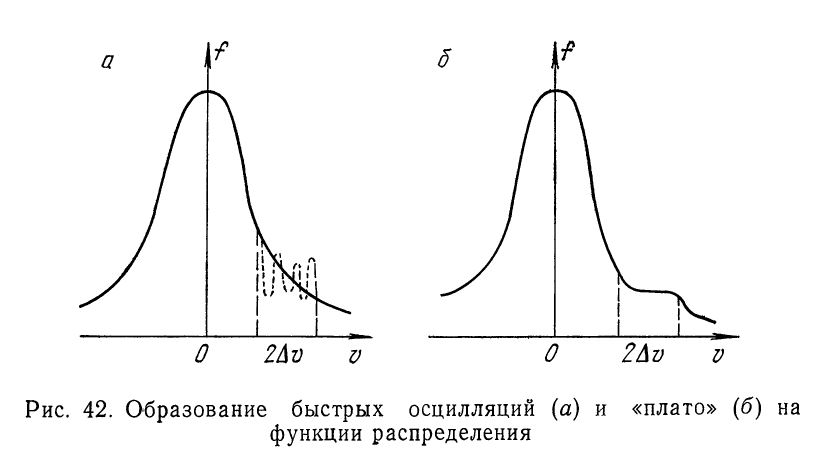
\includegraphics[width=70mm]{zatuh_landau_nonlinear_2.JPG}}
	%\caption{\label{fig.2.4.1}}
\end{figure}
\begin{figure}[h!]
	\center{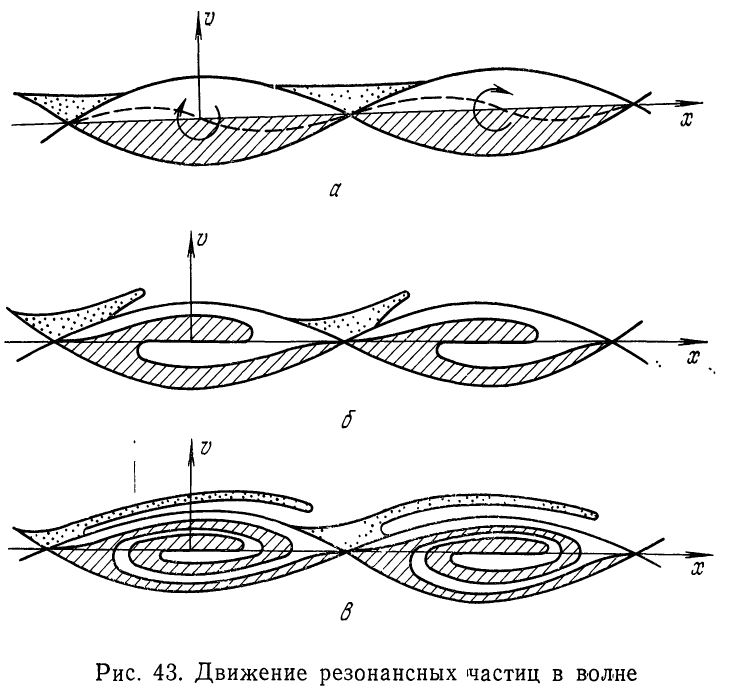
\includegraphics[width=70mm]{zatuh_landau_nonlinear_3.JPG}}
	%\caption{\label{fig.2.4.1}}
\end{figure}


Т.е. течение по f является несжимаемым. То есть f сохраняется вдоль линии тока. Поэтому, захваченные частицы с разбросом от $v_{phase} - \Delta v$ до  $v_{phase}+\Delta v$ будут иметь одну и ту же скорость, так как захваченные частицы быстро обмениваются энергией (из-за кулоновских столкновений, которые быстрее обычных столкновений).

Оценим амплитуду при которой можно считать волну нелинейной. Сравним плотность энергии в плоской волне:
\begin{equation}
	\varepsilon = \frac{E^{2}_0}{8 \pi} = \frac {k^2 \phi^{2}_0}{8 \pi}
\end{equation}
Энергия электронов в плато, ширина которого $\Delta v \sim \sqrt{e \phi_0 /m_e}$, а изменение энергии электрона при увеличении его скорости на $\Delta v$ вблизи фазовой скорости $\omega/k$ равно $m_e \Delta v \omega /k$ (по факту просто разложили $\frac{m(v+\Delta v)^2}{2}$).
Так как при образовании плато функция распределения меняется на величину:
\begin{equation}
	\Delta f \sim \frac{\delta f}{\delta v}|_{v=\omega/k} \Delta v
\end{equation}
Тогда изменение плотности энергии захваченных частиц по порядку величины равно:
\begin{equation}
	\Delta \varepsilon \sim m_e \frac{\omega}{k} \Delta v (\Delta f \Delta v ) \sim m_e (e \phi_0 /m_e)^{3/2} v \frac{\delta f}{\delta v}|_{v=\omega/k} 
\end{equation}
Вспоминаем, что у нас электроны имеют максвелловское распределение по скоростям, получаем:

\begin{equation}
	\sqrt{\frac{e \phi_0}{T_e}} \ll \frac{1}{(kd)^4} exp(-\frac{1}{2k^2 d^2})
\end{equation}

То есть при очень малых $kd$ даже оч малой амплитуды, может с собой много частиц уносить, и наоборот, при $kd > 1$ частиц будет мало


\subsection{Эхо в плазме. Аномальные диффузия, теплопроводность и сопротивление}

\subsubsection{Эхо в плазме.}
Самое первое эхо, которое обнаружили было спиновое эхо в экспериментах по ядерному резонансу. После двух импульсов с разницой в $\tau$ ответом от среды видели 3-й импульс, отстоящий на $\tau$.
\begin{figure}[h!]
	\center{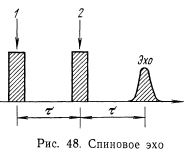
\includegraphics[width=70mm]{Echo_1_18.3.JPG}}
	%\caption{\label{fig.2.4.1}}
\end{figure}
Легче всего это увидеть на примере Циклотронного эха в плазме. Поперек столба созданной высокочастотным разрядом распадающейся плазмы, когда ток в ней практически отсутствовал и она была достаточно спокойной, пропускались два импульса высокочастотных колебаний с интервалом времени $\tau$. Плазма помещалась в магнитное поле около 3 кГс, а частота генератора была близка к циклотронной частоте электронов. Амплитуда импульсов была достаточно высокой, так что при циклотронном резонансе электроны могли приобретать энергию, значительно превышающую тепловую. После прохождения.
Что же происходило с точки зрения энергии электронов? Так как импульсы были довольно узкие, то из-за широкого спектра, он ВСЕ электроны приобретали одну и ту же энергию (скорость) (сдвиг на $v_p$ по диаграмме, рис. а.). После этого, электроны начинали вращаться с циклотронной частотой и скорость их стала не только по одной координате (из точки переросла в окружность с радиусом $v_p$). После того, как приходит второй импульс, то все электроны вновь смещаются на $v_p$ вдоль x (рис. в.). Эта смещённая окружность вновь должна расплыться по кругу вокруг (0;0) и будет иметь вид кривой на (рис. г.). 
\begin{figure}[h!]
	\center{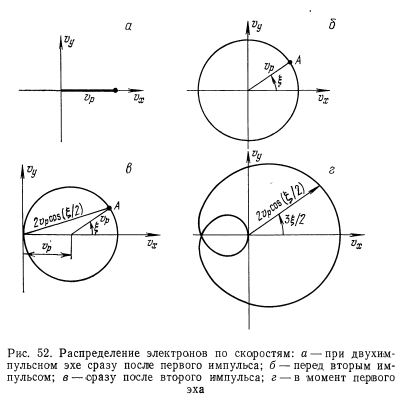
\includegraphics[width=70mm]{Echo_2_18.3.JPG}}
	%\caption{\label{fig.2.4.1}}
\end{figure}
Если будем следить за отдельными электронами, которые успели сдвинуться по фазе на $\xi$ в пространстве скоростей, то после второго импульса, они будут иметь скорость уже $2 v_p cos(\xi /2)$ и смещены на угол $\xi /2$ (см. рисунок). После времени $tau$ (за это время нужная пачка электронов повернулась на $\xi$) ВСЯ эта группа соберётся в точе отстающей по фазе на $3\xi/2 =\xi /2 + \xi $ .  А из рис. г. видно что может создавать эхо, но его не видно на картинке :D.
Чтобы циклотронное эхо проявилось, нужен нелинейный механизм. Это может быть релятивизим (масса от скорости) или зависимость частоты столкновений от скорости. Ну или трёхимпульсное эхо. 
\begin{figure}[h!]
	\center{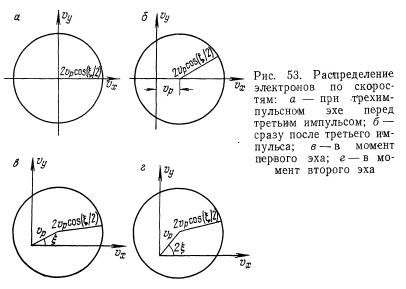
\includegraphics[width=70mm]{Echo_3_18.3.JPG}}
	%\caption{\label{fig.2.4.1}}
\end{figure}
Эхо может наблюдаться и на плазменных волнах.
На сетку, установленную в плазму подаётся сигнал с частотой значительно больше плазменной. Тогда и $\epsilon$ такой плазмы можно считать 1. В этом случае функцию распределения электронов можно представить как:
\begin{equation}
	f_1 (x,v,t)=f_1 (v) exp(-i \omega_1 t + i \omega_1 \frac{x}{v})
\end{equation}
, где  $f_1 (v)$ - амплитуда возмущения функции распределения вблизи сетки. Вид возмущения следует, что вдалеке это должно удовлетворять свободному движению частиц:
\begin{equation}
	\frac{\delta f_1}{\delta t} + v \frac{\delta f_1}{\delta x} =0
\end{equation}

Функцию распределения можно рассматривать как набор модулированных пучков, вблизи сетки они все по фазе колеблются, а по мере удаления - нет, поэтому плотность заряда
\begin{equation}
	\rho = -e \int f_1 dv
\end{equation}
должна быстро убывать при увеличении x.
ПУсть теперь на расстоянии d от сетки есть вторая, на которую подаётся переменный потенциал с частотой $\omega_2$ больше $\omega_{pe}$
Вторая сетка будет моделировать функцию $f_1$ так что появится нелинейный отклик $f_2$ на комбинационной частоте:
\begin{equation}
	f_2 (x,v,t)=f_2 (v) exp[-i \omega_1 (t-\frac{x}{v}) \pm i \omega_2 (t- \frac{x-d}{v})]
\end{equation}
При $x=d\frac{\omega_2}{\omega_2-\omega_1}$ экспонента, отвечающая частоте $\omega_2-\omega_1$ перестаёт зависеть от $v$. Это значит, что в точке
\begin{equation}
	x=d+d \frac{\omega_1}{\omega_2-\omega_1}=d  \frac{\omega_2}{\omega_2-\omega_1}
\end{equation}
должны наблюдаться заметные колебания плотности заряда на частоте $\omega^{,} = \omega_1-\omega_2 $ и зонд это может обнаружить.


\section{Нелинейные эффекты в плазме}

Какой-то текст 18

\subsection{Механизмы трехволнового взаимодействия в плазме. Примеры трехволновых процессов. Распадные неустойчивости. Соотношения Мэнли-Роу. Модифицированный распад. Процессы индуцированного рассеяния волн}

\subsubsection{Механизмы трехволнового взаимодействия в плазме. Примеры трехволновых процессов. Распадные неустойчивости. Соотношения Мэнли-Роу.}

Из уравнений Максвелла можно легко получить, что
\begin{equation}
	k^2 E - k (kE)+\frac{\omega^2}{c^2} D =0
\end{equation}
Но вот лучше добавить ток смещения (не самосогласованный ток) в правую часть
\begin{equation}
	k^2 E - \frac{c^2 k (kE)}{\omega}+\frac{\omega^2}{c^2} D =-\frac{4 \pi i \omega}{c^2} j_{s}
\end{equation}
так же сразу будем находить эл. поле как сумму по гармоникам
\begin{equation}
	E=\sum E_k exp(-i \omega_k t + ikr) + c.c.
\end{equation}
c.c. - комплексно сопряжённая часть.
Тогда для какой-то гармоники перепишется 

\begin{equation}
	\omega D_k - \frac{c^{2} k^{2}}{\omega} E_k + \frac{c^2 k(k E_k)}{\omega}=-4 \pi i j_{sk}
\end{equation}
Здесь $D=\hat{\epsilon} E$, вообще, у однородного этого уравнения имеются решения только совпадающих с собаственными частотами $\omega=\omega_k$. Да и чисто формально мы можем из D и $k^2-k(k e)$ по факту только перпендикулярная компонента можно сделать следующее:
\begin{equation}
	(\omega \epsilon - \frac{c^{2} k^{2}_{\perp}}{\omega}) E_k = -4 \pi i j_{sk}
\end{equation}
где $\epsilon=e^{*}_k \hat{\epsilon} e_k$, $k^{2}_{\perp}=k^{2}-|e_k k|^2$,$j_{sk}=e^{*}_k j_{sk}$
Вблизи $\omega=\omega_k$ левую часть вообще можно записать в виде множителя $A_k (\omega - \omega_k) E_k$.
\begin{equation}
	A_k=\frac{1}{\omega} \frac{\delta}{\delta \omega} (\omega^2 \epsilon) , \omega_k=\frac{ck_{\perp}}{\sqrt{\epsilon}}
\end{equation}
А для продольных волн с $k_{\perp}=0$ само $\epsilon$ обращается в 0 при   $\omega=\omega_k$ и величина $A_k= \omega \frac{\delta \epsilon}{\omega}$. То есть, уравнение перепишется:
\begin{equation}
	-i(\omega - \omega_k) E_k=-4 \pi i j_{sk}/A_k
\end{equation}
И действительно $E_k$ действительно велико вблизи $\omega=\omega_k$ и может даже расходиться в этой точке. Но это уравнение для фурье компоненты и фактически зависимость поля от времени:
\begin{equation}
	\int E_{\omega} exp(-i \omega t) d \omega
\end{equation}
Тогда $E_k (t) = \int E_{\omega} exp(-i \omega t) d \omega *exp(i \omega_k t)$ - это МЕДЛЕННАЯ амплитуда волны вблизи собственной частоты. То через фурье штуки получаем:
\begin{equation}
	\frac{\delta E_k}{\delta t} = \frac{4 \pi}{A_k} exp(i \omega_k t) j_{sk} (t)
\end{equation}
Тут $j_{sk} (t)$ сторонний ток как функция времени. То есть медленная амплитуда зависит от тока, который в свою очередь может зависеть от полей ВСЕХ гармоник. Вот тут и первый раз появляется нелинейность. Можно перейти к амплитудам волн и обезразмеренным операторам. То есть по факту:
\begin{equation}
	\frac{\delta a_k}{\delta t} =\sum_{k’} V_{k k^{,} k^{,,}} a_{^{,}} a_{k^{,,}} exp[-i(\omega_{k^{,}}+\omega_{k^{,,}}-\omega_k)] 
\end{equation}
Ну тут понятно, что из двух k’ и k’’ справа, должен получаться k, который слева, поэтому сразу ограничимся 3-мя волнами и запишем уравнения:
\begin{align}
	\frac{d a_1}{dt}=V1 a_2 a_3 \\
	\frac{d a_2}{dt}=V2 a_1 a^{*}_3 \\
	\frac{d a_3}{dt}=V3 a_1 a^{*}_2 \\
\end{align}
К.с. справа для того, чтобы выполнить $k_1=k_2+k_3’$ , $\omega_1=\omega_2+\omega_3$ . 
Умножим каждое уравнение на $\omega_i a^{*}_i$ и $k_i a^{*}_i$ и складывая их с к.с. получим законы сохранения энергии и импульса (соотношения Мейнли-Роу) 
\begin{align}
	\omega_1 |a_1|^2 + \omega_2 |a_2|^2 + \omega_3 |a_3|^2 = const \\
	k_1 |a_1|^2+ k_2 |a_2|^2 + k_3 |a_3|^2  = const \\	
\end{align}
Если взять какие-либо 2 уравнения и умножить их на недостающую комплексную амплитуду
\begin{align}
	\frac{d a_1}{dt} a^{*}_1=V1 a_2 a_3 a^{*}_1 \\
	\frac{d a_2}{dt} a^{*}_2=V2 a_1 a^{*}_3 a^{*}_2 \\
\end{align}
То ещё получится соотношение $a^{2}_1+a^{2}_2$.
Уравнение  $\omega_1 |a_1|^2 + \omega_2 |a_2|^2 + \omega_3 |a_3|^2 = const$ даёт нам поверхность эллипса в 3-х мерном пространстве,  $a^{2}_1+a^{2}_2$ - на поверхности этого эллипса выделит определённые линии, которые будут отвечать начальным условиям.
\begin{figure}[h!]
	\center{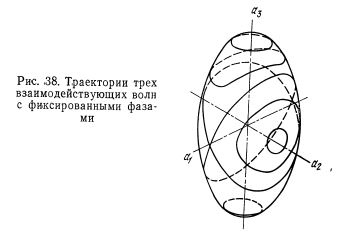
\includegraphics[width=70mm]{Wavetrans1.JPG}}
	%\caption{\label{fig.2.4.1}}
\end{figure}
Тут есть 2 вида траекторий, которые отвечают устойчивым и неустойчивым состояниям.
\begin{figure}[h!]
	\center{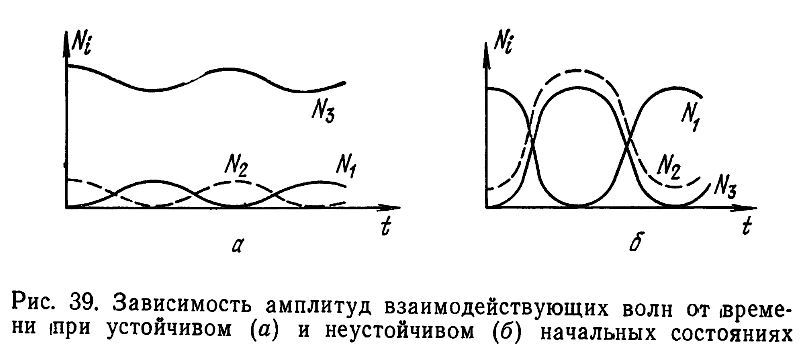
\includegraphics[width=70mm]{Wavetrans2.JPG}}
	%\caption{\label{fig.2.4.1}}
\end{figure}

\subsubsection{Модифицированный распад}
[М.В. Кузелов, Нелинейная теория излучения прямолинейным релятивистским пучком электронов в электростатическом поле накачки, ЖТФ, 1983, том 53, выпуск 6, 1029-1035]
Релятивистский пучок электронов, движущийся в периодическом поле, может быть источником когерентного коротковолнового излучения.
То есть, у нас есть волна периодического поля, есть “волна” электронного пучка, и они при сложении генерируют третью - волну рентгеновского излучения. 
При  модифицированном распаде механизмом насыщения неустойчивости является захват электронов комбинационной волной.(наблюдается при малой плотности электронов)




\subsection{Механизмы нелинейного самовоздействия волн в плазме (тепловые, силовые, ионизационные, релятивистские). Уравнения движения плазмы с учётом усреднённой силы со стороны высокочастотного поля. Модуляционная неустойчивость, ленгмюровские солитоны. Примеры самовоздействия электромагнитных волн в плазме (волноводные каналы, солитоны огибающих, ионизационное каналирование поверхностных волн)}

Какой-то текст 20

\subsection{Сильная и слабая турбулентность плазмы. Параметрическое возбуждение ионно-звуковой и ленгмюровской волн в высокочастотном поле. Генерация “кавитонов” в области плазменного резонанса. Ионно-звуковые солитоны. МГД и бесстолкновительные ударные волны}

\section{Излучение плазмы}

Для описания излучения будем пользоваться т.н. квазиклассическим приближениемб условие применимости которого имеет вид:

\begin{equation}
    |\frac{d \lambda_{db}}{dx}|\ll 1,
\end{equation}
которое, для случая кулоновского потенциала $U=-Ze^2/r$, записывается в известном виде:

\begin{equation}
    \frac{Ze^2}{\hbar v} > 1,
\end{equation}
где $v$ - скорость электрона. Также стоит отметить, что для инфинитной траектории это условие имеет вид:

\begin{equation}
    \frac{m \rho v}{\hbar} \approx l \gg 1,
\end{equation}
где $l$ - квантовое число кол-ва движения.

Полезно также знать форулу для мощности дипольного излучения зарядом e:

\begin{equation}
    Q(t) = \frac{2e^2}{3c^3}|\ddot{\mathbf{r}}(t)|^2.
\end{equation}

Также вводят т.н. эффективное излучение: $\Delta \kappa = \int_0^{\inf} E(\rho) 2\pi \rho d\rho$, можно знаписать свять
спектральной мощности злучения ($\kappa$ в одну гармонику) с сечением:

\begin{equation}
    \frac{d\sigma}{d\omega}=\frac{1}{\hbar\omega} \frac{d\kappa}{d\omega}.
\end{equation}

\subsection{Виды излучения: Тормозное, магнитотормозное, черенковское, переходное, комптоновское. Нормальный и аномальный эффект Доплера. Особенности излучения релятивистских электронов. Синхротронное излучение в плазме. Сила реакции излучения; давление излучения в плазме}
Тормозное излучение представляет из себя свободно - свободый переход, возникает при инфинитном движении. 
Спектральное излучение в пределе больших частот($\omega \gg mv^3/Ze^2$) есть:

\begin{equation}
    \frac{d\kappa}{d\omega}=\frac{4\pi}{3}\frac{Z^2 e^6}{m^2 c^3 v_i^2}.
\end{equation}
В обратном случае излучение будет дипольным и вырадение принимает вид:

\begin{equation}
    \frac{d\kappa}{d\omega}=\frac{16}{3}\frac{Z^2 e^6}{m^2 c^3 v_i^2} \ln\left(\frac{2mv^3}{\delta \omega e^2 Z} \right),
\end{equation}
где $\delta \approx 1.78$.

Возможно также будут спрашивать про т.д.р. случай. Тут, следуя закону Кирхгофа, $\kappa$ зависит только от температуры среды. Спектральная мощность излучения из плазмы дается выражением:

\begin{equation}
    dQ(\omega)=N_i N_e \hbar \omega d\kappa(\omega).
\end{equation}

Когда электрон движется под углом к магнитному полю, он излучает т.н. магнитотормозное излучение(не важно есть среда или
нет, это общий термин). Если частица нерелятивистская, то излучение называется циклотронным (оно похоже на дипольное). В
случае, когда электрон реляливистский(ультрарелятивистский?) питч угол $\theta \gg mc^2/\varepsilon$, излучение
называется синхротронным. Когда имеет место обратное неравенство на питч угол, излучение носит название - релятивистское
дипольное, в этом случае можно перейти в с.о., где у элетрона скорость вдоль матнитого поля ноль и в этой системе
излучение будет циклотронным. В области релятивизма (умеренного?) $\varepsilon\gg mc^2$ излучение называется
гиросинхротронным.

Получим выражение для гармонк, воспользовавшись законами сохранения:

\begin{equation}
    \sqrt(m^2c^4+p_m^2c^2) - \sqrt(m^2c^4+p_n^2c^2)=\hbar \omega,
\end{equation}

\begin{equation}
    p_{|| m} - p_{|| n} = \frac{\hbar\omega}{c}n_j \cos(\alpha),
\end{equation}
где индексы $m$, $n$ соответствуют состояниям до и после испускания соответственно, $n_j$ - пок. преломления, $\alpha$ -
угол между волновым вектором и магнитным полем. Используя известное выражение для уровней Ладау можно записать вырадение
для изменение поперечной энергии:

\begin{equation}
    (p_{\perp m}^2 - p_{\perp n}^2)/2m = s\hbar\omega_B,
\end{equation}
где $s = 0, \pm1, \pm2, ..$ - номер гармоники.

Уравнение для гармоник можно найти в [Железняков, (10.28)] (оно большое и никто его не знает, так что...). Для слабо-
релятивистского электрона в вакууме решение (10.28):

\begin{equation}
    \omega = \frac{s\omega_B + \hbar \omega^2/2mc^2 \sin^2(\alpha)}{1-\beta_{||}\cos(\alpha)},
\end{equation}
второе слагаемое в числителе есть т.н. эффект отдачи - изменение частоты излучения за счет продольного импульса и
поперечной энергии.

\begin{equation}
    \omega = \frac{s\omega_B \sqrt(1-\beta^2)}{1-\beta_{||}\cos(\alpha)}.
\end{equation}
Случай $n_j\beta_{||}\cos(\alpha)<1$, называется нормальным эффектом Доплера, в данном случае излучение кванта
сопровождается переходом частицы и состояния с большей поперечной энергией в состояние с меньшей. Случай $n_j\beta_{||}\cos(\alpha)>1$,
назывется аномальным эффектом доплера - легко видеть, что при излучении поперечная энергия растет, энергия на то и на 
другое черпается из продольного движения. Легко видеть, что показатель преломления должен быть больше 1.
Из-за этого эффекта в анизотропных средах может происходить раскачка коллебаний осциллятора.

Циклотронное излучение(наверо надо пару слов). Тут следующие приближения: $\beta^2\ll1$, $|n_j\beta_{||}|\ll1$,
$|\beta_{||}\omega\frac{\partial n_j}{\partial \omega}|\ll1$, $|sn_j\beta_{\perp}\sin(\alpha)|$. Циклотронное 
излучение происходит только в области нормального эффекта Доплера. Частота циклотронного излучения $\omega=s\omega_B$,
на первой гармонике излучение дипольное, дальше мультиполные.

Синхротронное излучение.
Тут важно помнить выражения для потенциалов Линеара-Вихерта:

\begin{equation}
    \mathbf{A}=\frac{e\mathbf{v}}{c(R-\mathbf{R}\mathbf{v}/c)},
\end{equation}

\begin{equation}
    \phi=\frac{e}{c(R-\mathbf{R}\mathbf{v}/c)},
\end{equation}
величины в правой части берутся в запаздывающий мометн времени $t-R/c$. Знаменатель можно записать как:

\begin{equation}
    R - \mathbf{R}\mathbf{v}/c=R(1-\beta\cos(\theta))\approx R(1-\beta+\theta^2/2),
\end{equation}
откуда видно, что потенциалы велики в направлениях $\theta \ll 1/\gamma$. Излучение происходит преимущественно в
направлении движения частицы в конус с раствором $1/\gamma$. Рассмотрим вращение частицы в постоянном магнитном поле. 
Частица вращается по окружности с периодом $2\pi\gamma/\omega_B$. Тогда длительность импутьса в лабораторной системе:
$\Delta t = \frac{1}{\gamma^2\omega_B}$. Таким образом характерная частота, на которой происходит излучение есть 
$\omega_c \approx \gamma^2\omega_B$. Сам спектр очень широкий и имеет экспоненциальный хвост на больших частотах.

Пусть теперь есть среда, если $n>1$, то излучение направлено в черенковский конус(а не в направлении скорости, как в 
вакууме).
Существенные изменения в излучении будут, если $n<1$, и $1-n\ll1$. Подставляя $n$ в потенциалы ЛВ получим, что
ширина спектра определяется $\theta \approx \sqrt(1-n\beta)$. Если при этом $1-n^2\gg1/\gamma^2$, то ширина диаграммы
определяется полностью средой т.е. $\theta\approx\sqrt(1-n)$. Теперь потенциалы не стремятся к бесконечности, при
$\beta ->\inf$, происходит "депрессия" излучения.

Переходное излучение.
Суть(остатьное тут огромные формулы, их переписывать смысла нет): Пусть есть два диэлектрика $\varepsilon_1$,
$\varepsilon_2$, граница раздела находится в $z=0$. В области $z>0$ движется заряд $q$ в направлении $-z$. При переходе
через границу сред возникает переходное излчение.
Физика излучения следующая. Пусть заряд $q$ покоится (в точке x, y, d), тогда, как известно, для нахождения
полей в областях $z>0 и z<0$ используют метод изображений - помещают заряд
$q'=-q\frac{\varepsilon_1-\varepsilon_2}{\varepsilon_1+\varepsilon_2}$ 
слева(в области $z<0, \varepsilon_1$) в точке x,y,-d. В области $z>0$ помещают 
заряд $q''=q\frac{2\varepsilon_1}{\varepsilon_1+\varepsilon_2}$.
Когда заряд пересекает границу раздела, его изображения, какбы, резко меняют направление, т.е. меняется скорость
(точнее отношение скорости заряда к фазовой скорости излучаемой волны), и происходит излучение. Это похоже на то,
как возикает излучение, при движении заряда над гофрированной поверхностью проводника - в данном случае изображение 
осциллирует.

Сила реакции излучения.
Суть по простому - частица излучает, а значит теряет энергию. Эти потери можно представить в виде некой силы трения
(правда есть нюансы). Рассмотрим частицу двигающуюся по кругу. Потенциал ЛВ имеет следующий вид:

Комптоновское рассеяние.
Это рассеяние фотона на электроне, строгие выражения получаются из квантовой теории поля, но момжно получить
некторою информаци. используя законы сохранения. Запишем закон сохранения импульса и энергии:

\begin{equation}
    \mathbf{p}_e=\mathbf{p}_{\gamma}-\mathbf{p'}_{\gamma},
\end{equation}

\begin{equation}
    E_e + E_{\gamma}=E_e' +E_{\gamma}',
\end{equation}
выполняя простые переобразования, легко получить выражение для изменения длины волны:

\begin{equation}
    \lambda'-\lambda=\frac{\hbar}{2\pi mc} (1-\cos(\theta)),
\end{equation}
где угол $\theta$ есть угол между начальным и конечным импульсами фотона.

Давление в плазме (я ничего не нашел  в учебниках)
Давление эм волны определяется как:

\begin{equation}
    P = 2\frac{<S>}{c} = 2\frac{I}{c},
\end{equation}
где $I$ - интенсивность, или усредненный вектор пойнтинга. Можно записать вектор пойнтинга для среды с дисперсией:

\begin{equation}
    \mathbf{S}=\mathbf{S}_E-\frac{1}{16\pi}\frac{\partial}{\partial\mathbf{k}}(\varepsilon\omega)|E|^2-\frac{1}{16\pi}\frac{\partial}{\partial\mathbf{k}}(\mu\omega)|H|^2
\end{equation}


\begin{equation}
    \mathbf{A}=\frac{\mathbf{j}_0}{cr} \exp(ikr - i\omega t),
\end{equation}
запишем фурье компоненту для поля: 

\begin{equation}
    \mathbf{E}=ik_0\mathbf{A}+i/k_0 \grad div(\mathbf{A}),
\end{equation}
где $k_0=\omega/c$. После вычислений имеем:

\begin{equation}
    \mathbf{E}=\left( 
    \frac{ik_0\mathbf{r}\times[\mathbf{j}_0\times \mathbf{r}]}{cr^3} +
    \mathbf{j}_0\cdot\mathbf{r}\frac{3\mathbf{r}}{cr^4} - \mathbf{j}_0/(cr^2) +
    \frac{3i}{k_0c}\frac{\mathbf{j}_0\cdot\mathbf{r} \mathbf{r}}{r^5} - \frac{i\mathbf{j}_0}{k_0 cr^3}
              \right) \exp(ik_0r-i\omega t),
\end{equation}
видно, что есть 3 типа зависимости: $k_0/r, 1/r^2, 1/(k_0r^3)$. Рассмотрим поле около частицы (раскладываем экспоненту
по $k_0r$). Третье слагаемое в экспоненте даст в совокумности член, в котором нет особености в $r=0$, этот член 
имеет вид:

\begin{equation}
    \mathbf{E}_3=-\frac{2}{3}\frac{k_0^2}{c}\mathbf{j}_0\exp(-i\omega t) = \frac{2}{3c^3} \dddot{\mathbf{p}},
\end{equation}
Зная поле, можно записать силу, действующую на частицу и умножив на скорость и усреднив ее по периоду, получим

\begin{equation}
    P=<\mathbf{F}\mathbf{v}>=-\frac{2}{3c^3}|\ddot{\mathbf{p}}|^2,
\end{equation}
знакомая формула диполного излучения. Однаком мы говорим о силе: для нерелятивистского электрона можно записать уравнение

\begin{equation}
    m\dot{\mathbf{v}}=e\mathbf{E}+\frac{e}{c}[\mathbf{v}\times\mathbf{B}] + \frac{2e^2}{3c^3}\ddot{\mathbf{v}},
\end{equation}
это уравнение справедливо, когда сила трения много меньше силы Лоренца. Оно дает нефизичные решения (типа, когда
частица вылетает из области поля в свободное пр-во, но продолжает набирать скорость). Ограничение на силу можно
переписать $\lambda \gg e^2/mc^3$, т.е. мы не должны рассматривать процессы меньше некого радиуса. Это вообще 
довольно общие органичение на классическую электродинамику (его наверно лучше просто запомнить и не збивать голову
квантами).

\subsection{Тепловое и нетепловое излучения плазмы. Уравнение переноса излучения. Реабсорбция излучения, связь коэффициента поглощения и излучательной способности среды, метод коэффициентов Эйнштейна. Усиление излучения в неравновесной плазме. Вынужденное излучение из плазмы, в которой заданы начальные электронные токи}

Тепловое излучение есть эм излучение, генерируемое за счет энергии теплового движение частиц излучающего тела. Это
излчение удовлетворяет закону Кирхгофа - отношение излучающей способности, к его поглощающей зависит только от температуры
Излучение в основном генерируется электронами. Особенностью такого излучения является экспоненциальный спад
интенсивности на боьших частотах $I\sim \exp(-\hbar\omega/T)$.

Нетепловое - все остальное излучение, происходящее в неравновестных условиях.

Уравнение переноса излучения.
Явление переноса излучения с интенсивностью $I(\omega)$ характеризуется балансом процессов испускания и поглощения
квантов вдоль пути распространения излучения:

\begin{equation}
    \frac{dI(\omega)}{dx}=j(\omega)-\kappa(\omega)I(\omega),
\end{equation}
где $j$ - спонтанная излучательная способность, $\kappa$ - коэффициент поглоцения(с учетом индуцированного испускания).
Например, если есть атом с уровнями 1 и 0, и населеностями $N_0, N_1$, то:

\begin{equation}
    j(\omega)=N_1 A_{10}\hbar \omega G(\omega),
\end{equation}
где $A_{10}$ - коэффициент эйштейна спонтаного излучения, и $G$ - профиль линии излучения. Коэффициент поглощения:

\begin{equation}
    \kappa(\omega)=\hbar\omega (N_0 B_{01} - N_1 B_{10})G(\omega),
\end{equation}
где $B_{01}, B_{10}$ - коэффициенты эйнштейна для поглощения и индуцированного испускания. Связь коэффициентов:

\begin{equation}
    \frac{A_{10}}{B_{10}}=\frac{\hbar\omega_0^3}{\pi^2c^3},
\end{equation}

\begin{equation}
    \frac{B_{01}}{B_{10}}=\frac{g_1}{g_0},
\end{equation}
где $\omega_0$ - частота перехода между 1 и 0, $g_1, g_0$ - стат. веса уровней.

Если среда в тд равновесии, то следуя закону Кирхгофа:

\begin{equation}
    \frac{j}{\kappa}=\frac{\hbar\omega^3}{4\pi^3c^2}\frac{1}{\exp(\hbar\omega/T)-1}=B_{pl}.
\end{equation}

Оптическая толщина $d\tau=\kappa(\omega_0)dx$ - оптическая толщина среды. Обычно уравнение записывают так:

\begin{equation}
    \frac{dI(\omega)}{\tau}=-I(\omega) + S(\omega),
\end{equation}
где
\begin{equation}
    S(\omega) = \frac{N_1 A_{10}}{N_0 B_{01} - N_1 B_{10}}.
\end{equation}

Если среда в т.д. равновесии, и $N_1$ не зависит от координаты. Тогда можно найти интесивность:

\begin{equation}
    I(\omega) = B_{pi}\left( 1 - \exp(-L\frac{j}{B_{pl}})\right),
\end{equation}
откуда видно, что при большой толщине среды $L$ излучение определяется формулой плазмы. Если среда тонкая, то 
$I(\omega)\approx j(\omega)L$.

Усиление излучения в неравновесной плазме.



\subsection{Рассеяние электромагнитных волн на флуктуациях плотности плазмы}

Какой-то текст 23b

\section{Специальные разделы физики плазмы}
\subsection{Ускорение частиц. Ускорение на кильватерной волне и волне биений}

\newpage
\addcontentsline{toc}{section}{Список литературы}
\bibliographystyle{unsrt}
\bibliography{program.bib}

\end{document}
